\documentclass[a4paper, 12pt]{report}

\usepackage[dvipsnames]{xcolor}

%%%%%%%%%%%%%%%%
% Set Variables %
%%%%%%%%%%%%%%%%

\def\useItalian{0}  % 1 = Italian, 0 = English

\def\courseName{Machine Learning}

\def\coursePrerequisites{Sufficient knowledge of calculus, probability and algorithm design}

\def\book{\curlyquotes{Machine Learning}, Tom Mitchell}

\def\authorName{Simone Bianco}
\def\email{bianco.simone@outlook.it}
\def\github{https://github.com/Exyss/university-notes}
\def\linkedin{https://www.linkedin.com/in/simone-bianco}

% \def\authorName{Alessio Bandiera}
% \def\email{alessio.bandiera02@gmail.com}
% \def\github{https://github.com/aflaag-notes}
% \def\linkedin{https://www.linkedin.com/in/alessio-bandiera-a53767223}

%%%%%%%%%%%%
% Packages %
%%%%%%%%%%%%

\usepackage{../../packages/Nyx/nyx-packages}
\usepackage{../../packages/Nyx/nyx-styles}
\usepackage{../../packages/Nyx/nyx-frames}
\usepackage{../../packages/Nyx/nyx-macros}
\usepackage{../../packages/Nyx/nyx-title}
\usepackage{../../packages/Nyx/nyx-intro}

%%%%%%%%%%%%%%
% Title-page %
%%%%%%%%%%%%%%

\logo{../../packages/Nyx/logo.png}

\if\useItalian1
    \institute{\curlyquotes{\hspace{0.25mm}Sapienza} Università di Roma}
    \faculty{Ingegneria dell'Informazione,\\Informatica e Statistica}
    \department{Dipartimento di Informatica}
    \ifdefined\book
        \subtitle{Appunti integrati con il libro \book}
    \fi
    \author{\textit{Autore}\\\authorName}
\else
    \institute{\curlyquotes{\hspace{0.25mm}Sapienza} University of Rome}
    \faculty{Faculty of Information Engineering,\\Informatics and Statistics}
    \department{Department of Computer Science}
    \ifdefined\book
        \subtitle{Lecture notes integrated with the book \book}
    \fi
    \author{\textit{Author}\\\authorName}
\fi


\title{\courseName}
\date{\today}

% \supervisor{Linus \textsc{Torvalds}}
% \context{Well, I was bored\ldots}

%%%%%%%%%%%%
% Document %
%%%%%%%%%%%%

\begin{document}
    \maketitle

    % The following style changes are valid only inside this scope 
    {
        \hypersetup{allcolors=black}
        \fancypagestyle{plain}{%
        \fancyhead{}        % clear all header fields
        \fancyfoot{}        % clear all header fields
        \fancyfoot[C]{\thepage}
        \renewcommand{\headrulewidth}{0pt}
        \renewcommand{\footrulewidth}{0pt}}

        \romantableofcontents
    }

    \introduction

    %%%%%%%%%%%%%%%%%%%%%

    \chapter{Introduction to Machine Learning}

    \section{What is \curlyquotes{Machine Learning}?}

    While many common tasks can be easily solved by computers through an algorithm, some are hard to formalize as a series of steps to be executed in a deterministic way. As an analogy, consider how language is made of syntax and semantics. Syntax can easily be formalized as a sequence of sub-structures that make up a phrase. If a sentence is slightly malformed, the machine can have a hard time trying to reconstruct the correct syntax, but in most cases this can be achieved. For semantics, instead, we have a whole different problem: some words could have more meanings, giving sentences different interpretations depending on the context of the conversation. This task is clearly harder for a machine. Sometimes, not even humans are capable of solving it!

    In the past, these type of tasks where solved through \textit{expert systems}, that being any system programmed by a human expert to solve a specific task. Expert systems can be viewed as a sequence of if-else conditions: if the task requires $x$ then do $y$, and so on. Not all tasks can be solved through expert systems. In particular, some tasks need different solutions for many cases, making these primitive systems useless due to all cases being impossible to program.

    To solve this type of complex and variable tasks, we use \textbf{machine learning}, which slowly teaches the machine how to solve the problem in the best way possible. The idea here is to program computers in a way that improves a specific \textit{performance criterion} through \textit{example data} and \textit{past experiences}.

    Machine learning uses \textbf{data mining} --- the act of producing knowledge from known data --- to increase the experience of the machine in solving the designed problem. In general, machine learning comes in handy when one of the following conditions holds:
    \begin{itemize}
        \item There is no human expertise on the task
        \item Human experts are unable to explain their expertise
        \item The solution needs to adapt to particular cases
    \end{itemize}

    The field of machine learning had an exponential growth in recent years due to the growing flood of online data --- the so called \textit{big data phenomenon} --- and the increase of computational power to process such data through advanced algorithms based on theoretical results. First, we give a formal definition of a \textit{learning problem}.

    \begin{frameddefn}{Learning problem}
        A \textbf{learning problem} is the improvement over a task $T$ with respect to a performance measure $P$ based on experience $E$.
    \end{frameddefn}

    For example, suppose that we want to program a machine that learns how to play checkers. We define the learning problem as:
    \begin{itemize}
        \item The task $T$ is to play checkers
        \item The performance measure $P$ is the percentage of games won in a tournament
        \item The experience $E$ is the opportunity to play against self
    \end{itemize}

    But how can we improve such performance measure? What \textit{exactly} should the machine learn? These questions reduce the learning problem to finding a valid mathematical representation of $T$, $P$ and $E$.  The training process can be described by four phases:
    \begin{enumerate}
        \item The human expert suggests what is an optimal move for each configuration of the board
        \item The human expert evaluates each configuration, ranking them by optimality
        \item The computer plays against a human an automatically detects with configurations lead to a win, a loss or a draw
        \item The computer plays against itself to improve performance
    \end{enumerate}

    Formally, this whole process can be expressed as a simple mathematical function called \textbf{target function}. In particular, we want to choose a target function that represents the learning problem in the best way possible and that can be computed by a machine.

    For instance, consider the function $V : \mathrm{Board} \to \R$, defined as follows:
    \begin{itemize}
        \item If $b$ is a final board state and it is a win then $V(b) = 100$
        \item If $b$ is a final board state and it is a loss then $V(b) = -100$
        \item If $b$ is a final board state and it is a draw then $V(b) = 0$
        \item If $b$ is not a final board state then $V(b) = V(b^*)$, where $b^*$ is the best final board state that can be achieved starting from the board $b$ playing the optimal moves
    \end{itemize}

    This function perfectly models our learning problem. However, it cannot be computed by any program since we haven't defined what an optimal set of moves is. We need a new definition that encodes this concept of optimal strategy for a checkers game.
    
    For example, we can re-define $V$ as follows:
    \[V(b) = w_0 + w_1 \cdot \mathrm{bp}(b) + w_2 \cdot \mathrm{rp}(b) + w_3 \cdot \mathrm{bk}(b) +w_4 \cdot \mathrm{rk}(b) + w_5 \cdot \mathrm{bt}(b) + w_6 \cdot \mathrm{rt}(b)\]

    where:
    \begin{itemize}
        \item $\mathrm{bp}(b)$ is the number of black pieces
        \item $\mathrm{rp}(b)$ is the number of red pieces
        \item $\mathrm{bk}(b)$ is the number of black kings
        \item $\mathrm{rk}(b)$ is the number of red kings
        \item $\mathrm{bt}(b)$ is the number of red pieces threatened by black pieces
        \item $\mathrm{rt}(b)$ is the number of black pieces threatened by red pieces
    \end{itemize}

    With this formulation, we have reduced the concept of learning checkers to estimating the best possible values of the coefficients $w_1, \ldots, w_6$, which care called \textbf{weights}, that maximize the value of $V(b)$ for any board state $b$. This estimation process is referred to as \textit{learning the function $V$}.

    \begin{frameddefn}{Learned function}
        Given a target function $f : X \to Y$ with weights $w_1, \ldots, w_k$, we define the \textbf{learned function} $\widehat{f} : X \to Y$ as the current approximation of $f$ computed by a learning algorithm.
    \end{frameddefn}

    By definition, the learned function $\widehat{f}$ will never be equal to the target function $f$: the target function's weights are \underline{always unknown} by definition. The idea here is to approximate $f$ by repeatedly applying small changes to the weights $\widehat{w_1}, \ldots, \widehat{w_k}$ of $\widehat{f}$ in order to estimate the weights of $f$. To learn a function $f$, we need a \textit{dataset}. A dataset is a set of instances that can be used by a learning algorithm to improve the performance of the learned function.
    
    \begin{frameddefn}{Dataset}
        Let $f : X \to Y$ be a target function and let $f_{\mathrm{train}}(x)$ be the training value obtained by $x$ in the training data. Given a set of $n$ training inputs $X_D = \{x_1, \ldots, x_n\}$, the \textbf{dataset} of the learning problem is the set of samples defined as:
        \[D = \{(x_i, f_\mathrm{train}(x_i)) \mid x_i \in X_D\}\]
    \end{frameddefn}

    After training, the learned function $\widehat{f}$ will have learned the values of the inputs in the dataset, returning a value as close as possible to the one in the dataset (in some cases the returned value is exactly the same). However, we are interested in estimating the \textit{other} possible inputs, i.e. those that aren't in the dataset.

    In summary, a machine learning problem is the task of learning a target function $f : X \to Y$ through a dataset $D$ for a set $X_D$ of $n$ inputs. To learn a function $f$ means computing an approximating function $\widehat{f}$ that returns values as close as possible to $f$, especially for values outside of the dataset $D$, implying that $\forall x \in X - X_D$ it should hold that $f(x) \approx \widehat{f}(x)$. In order for the learned function to be \textit{good}, the set of training inputs $X_D$ must be very very small compared to the set of total inputs, meaning that $\abs{X_D} \lll \abs{X}$.

    There are distinct types of machine learning problems based on:
    \begin{itemize}
        \item The type of dataset used:
        \begin{enumerate}
            \item \textbf{Supervised learning}: problems where the model learns patterns from labeled data. Here, the dataset corresponds to $D = \{(x_i,y_i) \mid i \in X_D\}$, where $y_i$ is the sample of the function value for $x_i$
            \item \textbf{Unsupervised learning}: problems where the model learns patterns from unlabeled data. Here, the dataset corresponds to $D = \{x_i \mid i \in X_D\}$
            \item \textbf{Reinforcement learning}: problems in which an agent learns to make decisions by interacting with an environment and receiving rewards or penalties based on its actions.
        \end{enumerate}

        \item The type of function to be learned:
        \begin{enumerate}
            \item \textbf{Discrete Classification}: the input set is $X = A_1 \times \ldots \times A_n$, where $A_i$ is a finite set, and the output set is $Y = \{C_1, \ldots, C_k\}$. When $k = 2$, i.e. we have only two classes, we say that the problem is a \textbf{Concept Learning} problem
            \item \textbf{Discrete Regression}: the input set is $X = A_1 \times \ldots \times A_n$, where $A_i$ is a finite set, and the output set is $Y = \R^m$.
            \item \textbf{Continuous Classification}: the input set is $X = \R^n$ and the output set is $Y = \{C_1, \ldots, C_k\}$.
            \item \textbf{Continuous Regression}: the input set is $X = \R^n$ and the output set is $Y = \R^m$.
        \end{enumerate}
    \end{itemize}

    Classification problems are based on the classification of inputs into predetermined categories, while regression problems involve the approximation of functions defined over $\R$. Reinforcement learning, instead, is used for dynamic systems with unknown or partially known evolution model, usually robotic tasks and game playing. 
    
    \newpage

    \section{Hypotheses, consistency and representation}

    After discussing the basic notation and terminology, we are ready to deepen our understanding on how to learn a problem.
    
    \begin{frameddefn}{Hypothesis space}
        Given a target function $f$, an \textbf{hypothesis space} $H$ for $f$ is a set of functions $h \in H$, where $h$ is called hypothesis, that can be learned in order to reach an approximation of $f$.
    \end{frameddefn}

    The representation of a hypothesis space highly depends on the type of problem. For instance, consider the problem of classifying natural numbers into primes numbers and composite numbers. This corresponds to a discrete classification problem with two classes $\Primes$ and $\N-\Primes$, i.e. a concept learning problem where we want to learn the concept of prime number. The target function of the problem is thus described as $f : \N \to \{\Primes,\N-\Primes\}$. Here, the simplest hypothesis space is the set $H = \{h_A : \N \to \{A, \N-A\} \mid A \subseteq \N\}$.

    Given a performance measure $P$ over a dataset $D$ and a hypothesis space $H$, the learning task is to find the best approximation $h^* \in H$ of the function $f$ using the dataset $D$.
    \[h^* \in \argmax_{h \in H} P(h,D)\]

    Finding such optimal hypothesis is the core of a learning problem. However, by definition, a hypothesis space may also contain hypotheses that are clearly a wrong approximation of $f$ over $D$. For instance, given a dataset $D$ for a target function $f$, for any hypothesis $h \in H$ we can check wether $h(x) = f(x)$ only for instances $x \in X_D$ since the other values are unknown in $D$. This means that some hypothesis may have some values that are \textit{inconsistent} with the dataset itself, making them useless in the learning process. A hypothesis $h \in H$ is said to be \textbf{consistent} with a dataset $D$ of a target function $f$ if and only if $h(x) = f(x)$ for all $x \in X_D$. The subset of hypothesis that are consistent with a dataset is called \textbf{version space}. 

    \begin{frameddefn}{Version space}
        The \textbf{version space} of a target function $f$ with respect to the hypothesis space $H$ and the dataset $D$, written as $\mathrm{VS}_{H,D}$, is the subset of $H$ that contains all the hypotheses that are consistent with $D$.
        \[\mathrm{VS}_{H,D} = \{h \in H \mid \forall x \in X_D \;\; h(x) = f(x)\}\] 
    \end{frameddefn}

    Consider again the previous example. Suppose that we're working with the following dataset $D = \{(1, \N-\Primes), (3, \Primes), (5, \Primes), (6, \N-\Primes), (7, \Primes), (10, \N-\Primes) \}$. Here, the version space would restrict our interest to all those functions $h_A : \N \to \{A, \N-A\}$ where the elements $3,5,7$ lie inside $A$ and the elements $1,6,10$ lie outside of $A$.
    \[VS_{H,D} = \{h_A : \N \to \{A, \N-A\} \mid \{3,5,7\} \subseteq A \subseteq \N \text{ and } \{1,6,10\} \subseteq \N-A\}\]

    By definition, the best approximation for a performance measure $P$ over a dataset $D$ and a hypothesis space $H$ must clearly lie inside the version space $VS_{H,D}$. Hence, we can restrict our interest to the version space itself.
    \[h^* \in \argmax_{h \in VS_{H,D}} P(h,D)\]

    The concept of version space is based on the \textbf{inductive learning hypothesis}: any hypothesis that is consistent with the target function over a dataset of \textit{adequate size} will also approximate the target function well over other unobserved examples. In other words, if we consider a dataset of adequate size then every hypotheses inside the version space will be a nice approximation of the target function. 
    
    The simplest way to compute the version space is through the \textbf{List-Then-Eliminate} algorithm, a bruteforce algorithm that enumerates all the hypothesis space and then test the consistency of each hypothesis, discarding the invalid ones. Even though this algorithm is correct, it is also clearly \textit{infeasible} since enumerating all the different hypothesis would require an exponential amount of time. We'll see improved ways to compute the version space given by a dataset.

    \begin{framedalgo}[label={lte}]{List-Then-Eliminate}
        Given a hypothesis space $H$ and a dataset $D$, the algorithm returns $VS_{H, D}$
        \begin{algorithmic}
            \Function{listThenEliminate}{$H$, $D$}
                \State $VS_{H, D} := H$
                \For{$(x, f(x)) \in D$}
                    \State $H' := \{h \in H \mid h(x) \neq f(x)\}$
                    \State $VS_{H, D} = VS_{H, D} - H'$
                \EndFor
                \State \tbf{return} $VS_{H,D}$
            \EndFunction
        \end{algorithmic}
    \end{framedalgo}

    \subsection{Representation power and generalization power}
    
    In order for the inductive learning hypothesis to hold, the size of the dataset is a \textbf{critical} factor: if the hypothesis space is too \textit{powerful} and the search is complete, then the system won't be able to classify new instances, meaning that we have no generalization power.

    For instance, consider a generic concept learning problem described by the target function $c : X \to \{0,1\}$. Let $D$ be the chosen dataset. For any hypothesis space $H$, it's easy to see that $H$ is actually \textit{associated} with a particular set of instances, that being all instances that are classified as positive by such hypothesis. In fact, we have a mapping $\phi$ between the hypothesis space $H$ and the power set $\mathcal{P}(X)$.
    \[\phi_H : H \to \mathcal{P}(X) : h_A \mapsto A = \{x \in X \mid h_A(x) = 1\}\]

    In general, this mapping is not surjective, meaning that there is a subset $A$ of $\mathcal{P}(X)$ that is is not covered by a hypothesis inside $H$. In fact, we prefer cases where such mapping \underline{is not} surjective. This is known as the \textbf{hypothesis space representation issue}: some hypothesis spaces may be useless even when we restrict our interest to the version space.
    
    For example, suppose that there is a hypothesis spaces $H_1, H_2$ such that $H_1$ cannot represent $\mathcal{P}(X)$, i.e. $\phi_{H_1}$ is not surjective, while $H_2$ can:
    \begin{itemize}
        \item In $VS_{H_1,D}$ we have that $\exists x \in X-X_D$ for which there are two hypotheses $h, h' \in \mathrm{VS}_{H_1,D}$ such that $h(x) = 0$ and $h'(x) = 1$.
        \item In $VS_{H_2,D}$ we have that $\forall x \in X-X_D$ there are two hypotheses $h, h' \in \mathrm{VS}_{H_2,D}$ such that $h(x) = 0$ and $h'(x) = 1$.
    \end{itemize}
    
    The small difference in the quantifier has enormous impacts on the usefulness of these two spaces. If we use $H_1$ then we expect that the approximation found by any algorithm will give the wrong value for some unlabeled inputs $x \in X -X_D$ due to the presence of two functions that can be chosen for $x$. If we use $H_2$, instead, we expect that every unlabeled input will have a wrong value.
    
    These observations imply that the \textit{more information} the hypothesis space encapsulates about the values in $X_D$, the \textit{harder} it becomes to \textbf{generalize} and predict values for samples outside $X_D$. In other words, a more expressive hypothesis space can \textbf{overfit} to the data, making it more difficult to make accurate predictions on unsampled data. We'll return on the problem of overfitting the dataset in following sections.

    The process of reducing the \textit{representation power} of the hypothesis space in favor of \textit{generalization power} -- as in reducing the hypothesis space from $H'$ to $H$ in the previous example -- is called \textbf{language bias}. Ideally, we want our hypothesis space to be as good as possible. Clearly, the best possible hypothesis space contains only the optimal approximating function $h^* \in H$. In this case, the previous observations regarding the hypothesis space representation issue are solved: every unlabeled data will have only one value inside the function. The process of selecting one particular hypothesis among the set of possible ones -- i.e., choosing $h^* \in H$ -- is called \textbf{search bias}.

    In machine learning, the concept of learning bias is crucial for improving a model's ability to generalize. A good learning bias helps guide the learning algorithm towards patterns in the data that are useful for predicting unseen samples, increasing the system's generalization power. This bias allows the model to make accurate predictions on new data that wasn't part of the training set. Without such a bias, a system would simply \textbf{memorize} the dataset, failing to predict values for samples outside the training set, rendering it \textit{ineffective} in real-world applications. Systems lacking generalization capabilities would be of little use, as they wouldn't be able to provide meaningful predictions beyond the data they were trained on.

    In real-world applications, datasets often contain \textbf{noise}, which refers to irrelevant or erroneous information that can distort the true underlying patterns in the data. Noise can come from a variety of sources, including measurement errors, data entry mistakes, incomplete data or random fluctuations in the system being studied. This noise complicates the \textit{learning process}, as machine learning models may \textit{struggle} to distinguish between true \textit{signal} and \textit{noise}.

    A noisy data-point in a dataset $D$ for a function $f$ can be formulated as a pair $(x_i, y_i) \in D$, where $y_i \neq f(x_i)$. This means that there may be \tit{no consistent hypothesis} with noisy data, i.e. $\mathrm{VS}_{H, D} = \varnothing$. In these scenarios, \textbf{statistical methods} must be employed to implement robust algorithms, in order to reduce the noise in the data.

    \section{Performance evaluation}

    After discussing which hypotheses we're interested in, we'll now focus on evaluating the performance of a hypothesis. To give an intuition, we'll focus on classification problems. Let $f : X \to Y$ be a classification problem. Let $\mathcal{D}$ be a probability distribution over $X$, meaning that each element in $X$ has an associated probability of being drawn. The sum of all the probabilities in $\mathcal{D}$ must be 1. Let $S$ be a set of $n$ samples drawn from $X$ according to $\mathcal{D}$ and for which we know the value $f(x)$. By definition, $S$ corresponds to a dataset of $n$ random elements. For any possible hypothesis $h$ returned by a learning algorithm obtained through $S$, we want to know what is the best estimate of the \textit{accuracy} of $h$ over future instances drawn from the same distribution and what is the \textit{probable error} of this accuracy estimate. First, we have to define two error measures.

    \begin{frameddefn}{True error}
        Let $f : X \to Y$ be a classification problem. Given a hypothesis $h$, the \textbf{true error} of $h$ with respect to $f$ and a probability distribution $\mathcal{D}$ over $X$, written as $\mathrm{error}_\mathcal{D}(h)$, is defined as:
        \[\mathrm{error}_\mathcal{D}(h) = \Pr_{x \in \mathcal{D}}[h(x) \neq f(x)]\]
        The \textit{true accuracy} of $h$ is defined as $\mathrm{accuracy}_\mathcal{D}(h) = 1-\mathrm{error}_{\mathcal{D}}(h)$.
    \end{frameddefn}

    The true error of a hypothesis is clearly a perfect error measure. However, it's easy to see that computing the true error of $h$ is infeasible since we would have to compute such probability over all the inputs. To fix this, we consider another type of error measure that is less precise but computable.

    \begin{frameddefn}{Sample error}
        Let $f : X \to Y$ be a classification problem. Given a hypothesis $h$, the \textbf{sample error} of $h$ with respect to $f$ and a data sample $S$ over $\mathcal{D}$, written as $\mathrm{error}_S(h)$, is defined as:
        \[\mathrm{error}_\mathcal{S}(h) = \frac{1}{n} \sum_{x \in S} \delta(x)\]
        where $n=\abs{S}$, $\delta(x) = 1$ if $h(x) \neq f(x)$ and $\delta(x) = 0$ otherwise. The \textit{sample accuracy} is defined as $\mathrm{accuracy}_S(h) = 1-\mathrm{error}_{S}(h)$.
    \end{frameddefn}
    
    The sample error can be efficiently computed over a small data sample. The goal of a learning system is to be accurate in $h(x)$. However, sample accuracy may often fool us into thinking that our hypothesis is good: if $\mathrm{accuracy}_{S}(h)$ is very high but but $\mathrm{accuracy}_\mathcal{D}(h)$ is poor, our system is not be very useful.
    
    We also notice that, by definition, $\mathrm{error}_S(h)$ is actually a random variable depending on $S$. Sampling two different sets $S$ and $S'$ from $\mathcal{D}$ may different values for $\mathrm{error}_S(h)$ and $\mathrm{error}_{S'}(h)$. For this reason, we're also interested in the expected value $\Exp_{S \subseteq \mathcal{D}}[\mathrm{error}_S(h)]$ of the sample error, i.e. the weighted average over all the possible samples $S$. The \textbf{estimation bias} for $\mathcal{D}$ is defined as the difference between the expected sample error and the true error.
    \[\mathrm{bias}_\mathcal{D}(h) = \Exp_{S \subseteq \mathcal{D}}[\mathrm{error}_S(h)] - \mathrm{error}_\mathcal{D}(h)\]
    
    We notice that the estimation bias is equal to 0 if and only if $\Exp_{S \subseteq \mathcal{D}}[\mathrm{error}_S(h)] = \mathrm{error}_\mathcal{D}$. However, for any learning algorithm it is \textit{impossible} to prove that the bias is exactly 0. This derives from the very concept of learning function. Hence, in order for a hypothesis to be as good as possible, we want an estimation bias that is as close as possible to 0.
    
    If $S$ is the training set used to compute $h$ through some learning algorithm then $\mathrm{error_S}(h)$ will always be have some bias. In order to get an \textbf{unbiased estimate}, the training set $S$ used to compute $h$ and the evaluation set $S'$ must be chosen independently. However, even with an unbiased sample, $\mathrm{error}_{S'}(h)$ may still vary from $\mathrm{error}_{\mathcal{D}}(h)$ -- the smaller the set $S'$, the greater the expected variance.

    But how good is an estimate of $\mathrm{error}_\mathcal{D}(h)$ provided by a single $\mathrm{errors}_S(h)$? From the theory of statistical analysis, we can derive the concept of \textbf{confidence interval}. If $S$ contains $n$ samples drawn independently of one another over $\mathcal{D}$, $S$ is independent of $h$ and $n \geq 30$ then with approximately $N\%$ of probability we have that:
    \[\abs{\mathrm{error}_{S}(h) - \mathrm{error}_\mathcal{D}(h)} \leq z_N \sqrt{ \frac{\mathrm{error}_S(h)(1- \mathrm{error}_S(h))}{n}}\]
    where the value $z_n$ is a constant given by the \textit{confidence level} $N\%$.
    \begin{figure}[H]
        \centering
        \begin{tabular}{|c|ccccccc|}
            \hline
            $N\%$ & $50\%$ & $68\%$ & $80\%$ & $90\%$ & $95\%$ & $98\%$ & $99\%$ \\
            \hline
            $z_n$ & $0.67$ & $1.00$ & $1.28$ & $1.64$ & $1.96$ & $2.33$ & $2.58$ \\
            \hline
        \end{tabular}
        \caption{Relation between each confidence level and its constant}
    \end{figure}

    This result shows that a single sample error (when unbiased) is also a good estimation measure for the true error, up to some confidence level. However, in order to get a good approximation we must make some trade offs between \textit{training} and \textit{testing}:
    \begin{enumerate}
        \item Using more samples for training and less for testing gives a better approximating function $h$, but $\mathrm{error}_S(h)$ may not be a good approximation of $\mathrm{error}_D(h)$. 
        \item Using less samples for training and more for testing gives a worse approximating function $h'$, but $\mathrm{error}_S(h')$ is guaranteed to be a good approximation of $\mathrm{error}_D(h)$. 
    \end{enumerate}

    Usually, a good trade off for medium sized datasets is a training set of size $\frac{2}{3}\abs{X}$ and a testing set of size $\frac{1}{3}\abs{X}$. However, computing $\mathrm{error}_S(h)$ is not enough: the estimation bias is defined through $\Exp_{S \subseteq\mathcal{D}} [\mathrm{error}_S(h)]$. Computing the expected sample error is a task as hard as computing the true error. Nonetheless, thanks to the \textbf{central limit theorem}, the expected sample error can be easily approximated by averaging the computed values of $\mathrm{error}_{S_1}(h), \ldots, \mathrm{error}_{S_k}$, where $S_1, \ldots, S_k$ are independent from each other.
    \[\lim_{k \to +\infty} \overline{\varepsilon}_k - \Exp_{S \subseteq\mathcal{D}} [\mathrm{error}_S(h)] = 0 \implies \lim_{k \to +\infty} \overline{\varepsilon}_k = \Exp_{S \subseteq\mathcal{D}} [\mathrm{error}_S(h)]\]
    where $\overline{\varepsilon}_k = \frac{1}{k} \sum_{i \in [k]} \mathrm{error}_{S_i}(h)$. With all the tools that we have discussed, we're now ready to discuss our first unbiased estimator: the \textbf{K-Fold Cross Validation} algorithm.

    \begin{framedalgo}{K-Fold Cross Validation for Sample Error}
        Given a dataset $D$, a learning algorithm $L$ for a function $f$ and a value $k > 0$, the K-Fold Cross Validation returns an estimation $\mathrm{error}_{L,D}$ of the expected sample error of $L$ over $D$.
        \begin{algorithmic}
            \Function{kFoldCrossValidation}{$D,L,k$}
                \State{Partition $D$ into $k$ sets $S_1, \ldots, S_k$ where $\abs{S_i} > 30$}
                \For{$i$ = $1, \ldots, k$}
                    \State{$T_i$ = $D-S_i$}
                    \Comment{$T_i$ is the training set}
                    \State{$h_i$ = $L(T_i)$}
                    \State{$\delta_i$ = $\mathrm{error}_{S_i}(h_i)$}
                \EndFor
                \State{return $\frac{1}{k} \sum_{i \in [k]} \delta_i$}
            \EndFunction
        \end{algorithmic}
    \end{framedalgo}

    \subsection{Hypothesis comparison}

    Consider the case where we have two independent hypotheses $h_1$ and $h_2$ for some discrete-valued target function. Hypothesis $h_1$ has been tested on a sample $S_1$ and $h_2$ has been tested on an sample $S_2$. $S_1$ and $S_2$ are independent from each other and they are drawn from the same distribution $\mathcal{D}$. The difference $d$ between the true errors of these two hypotheses is given by 
    \[d = \mathrm{error}_\mathcal{D}(h_1) - \mathrm{error}_\mathcal{D}(h_2)\]

    The obvious choice for the estimator $\widehat{d}$ of $d$ is given by
    \[\widehat{d} = \mathrm{error}_{S_1}(h_1) - \mathrm{error}_{S_2}(h_2)\]

    In fact, it's very easy to prove that this is indeed an unbiased estimator.
    \[\Exp_{S \subseteq \mathcal{D}}[\mathrm{error}_{S}(h_1) - \mathrm{error}_{S}(h_2)] = \Exp_{S \subseteq \mathcal{D}}[\mathrm{error}_{S}(h_1)] - \Exp_{S \subseteq \mathcal{D}}[\mathrm{error}_{S}(h)] = d\]

    This definition of error comparison allows us to mathematically describe the concept of \textbf{overfitting}. In previous sections, we described this phenomenon as the property of a hypothesis of being too much expressive, i.e. it performs pretty good on the training data but it makes poor predictions on unsampled data.

    \begin{frameddefn}{Overfitting}
        Let $h \in H$ be a hypothesis for a function $f$ obtained through the training data $S$, where $H$ is the chosen hypothesis space. We say that $h$ \textbf{overfits} the set $S$ if there is an another hypothesis $h' \in H$ obtainable through $S$ that has a sample error higher than $h$ but a true error lower than $h$. 
        \[\mathrm{error}_S(h) < \mathrm{error}_S(h') \qquad \mathrm{error}_\mathcal{D}(h) > \mathrm{error}_\mathcal{D}(h')\]
    \end{frameddefn}

    Suppose that we have two learning algorithms $L_A$ and $L_B$. We want to determine which of them produces the best approximation of $f$ on average. The K-Fold Cross Validation algorithm that we discussed in the previous section can be easily adapted to compare $L_A$ and $L_B$.

    \begin{framedalgo}{K-Fold Cross Validation for Comparison}
        Given a dataset $D$, two learning algorithms $L_A, L_B$ for a function $f$ and a value $k > 0$, if the algorithm returns True then we expect that $L_A$ is better than $L_B$
        \begin{algorithmic}
            \Function{kFoldCrossComparison}{$D,L_A,L_Bk$}
                \State{Partition $D$ into $k$ sets $S_1, \ldots, S_k$ where $\abs{S_i} > 30$}
                \For{$i$ = $1, \ldots, k$}
                    \State{$T_i$ = $D-S_i$}
                    \Comment{$T_i$ is the training set}
                    \State{$h_i$ = $L_A(T_i)$}
                    \State{$h_i'$ = $L_B(T_i)$}
                    \State{$\delta_i$ = $\mathrm{error}_{S_i}(h_i) - \mathrm{error}_{S_i}(h_i')$}
                \EndFor
                \State{$\varepsilon$ = $\frac{1}{k} \sum_{i \in [k]} \delta_i$}
                \State{return $\varepsilon < 0$}
            \EndFunction
        \end{algorithmic}
    \end{framedalgo}

    \subsection{Performance metrics}

    Until now, we have focused on error and accuracy. Intuitively, we expect that if the accuracy is high, i.e. the error is low, then our hypothesis must be a good approximation. However, this is not always the case.

    For instance, consider a concept learning problem $f : X \to \{+,-\}$ with a training set where $90\%$ of the samples are negative, meaning that they are labeled with $-$. Consider the hypothesis $h$ that labels every single element $x \in X_D$ as negative. Even if this hypothesis is clearly bad, the accuracy would still be $90\%$. Of course, we're usually interested in the accuracy of approximations yield by learning models. In some cases, accuracy only is not enough to assess the performance of a classification method.

    In a more statistical sense, error and accuracy can be also described through the concept of positives and negatives:
    \begin{itemize}
        \item A \textbf{true positive} is a positive element that gets classified as positive
        \item A \textbf{true negative} is a negative element that gets classified as negative
        \item A \textbf{false positive} is a negative element that gets classified as positive
        \item A \textbf{false negative} is a positive element that gets classified as negative
    \end{itemize}

    Here, the error rate is described as the ratio between all the errors (false positives and false negatives) and all the samples:
    \[\mathrm{error} = \frac{\mathrm{FP} + \mathrm{FN}}{\mathrm{TP} + \mathrm{TN} + \mathrm{FP} + \mathrm{FN}}\]
    while the accuracy is still defined as the complement of the error.

    \begin{figure}[H]
        \centering
        \includegraphics[scale=0.25]{images/recall.png}
        \caption{The relevant elements are the elements that are really positive, while the retrieved elements are the ones that have been labeled as positive}
    \end{figure}

    As discussed in the example above, these two measures may be inappropriate when the datasets are unbalanced. For this reason, we also consider two additional measures. The first measure is the \textbf{recall} (also called \textit{true positive rate}), defined as the ratio between the true positives and the relevant elements. The recall measures the ability of the model to avoid false negatives.
    \[\mathrm{recall} = \frac{\mathrm{TP}}{\mathrm{TP} + \mathrm{FN}}\]

    The second measure is the \textbf{precision} (also called \textit{positive predictive value}), defined as the ratio between the true positives and the retrieved elements. The precision measures the ability of the model to avoid false positives.
    \[\mathrm{precision} = \frac{\mathrm{TP}}{\mathrm{TP} + \mathrm{FP}}\]

    The recall and the precision are usually used to compute the \textbf{F-score}, which  measures the predictive performance of a model. More formally, the $F_1$-score is the harmonic mean of the precision and recall. Thus, it symmetrically represents both precision and recall in one single metric.
    \[\mathrm{F_1} = \frac{2 \cdot \mathrm{recall} \cdot \mathrm{precision}}{\mathrm{recall} + \mathrm{precision}}\]

    Another very easy to read measure linked to classification errors is the \textbf{confusion matrix}. Given a classification problem $f : X \to Y$ and a hypothesis $h$ produced by a model for $f$, each row and column of the confusion matrix is labeled with the classes in $Y$. Each cell $c_{i,j}$ of a confusion matrix $C$ contains the number of samples whose true class is $C_i$ and whose class predicted by $h$ is $C_j$. When the confusion matrix produced by the analysis of the performance of a solution retrieved through an algorithm is \curlyquotes{accumulated} towards the central diagonal, the solution is a good model for the problem. Otherwise, the model is considered bad. The ratio between the sum of the main diagonal and the total number of samples corresponds to the accuracy of the model.

    \begin{figure}[H]
        \centering
        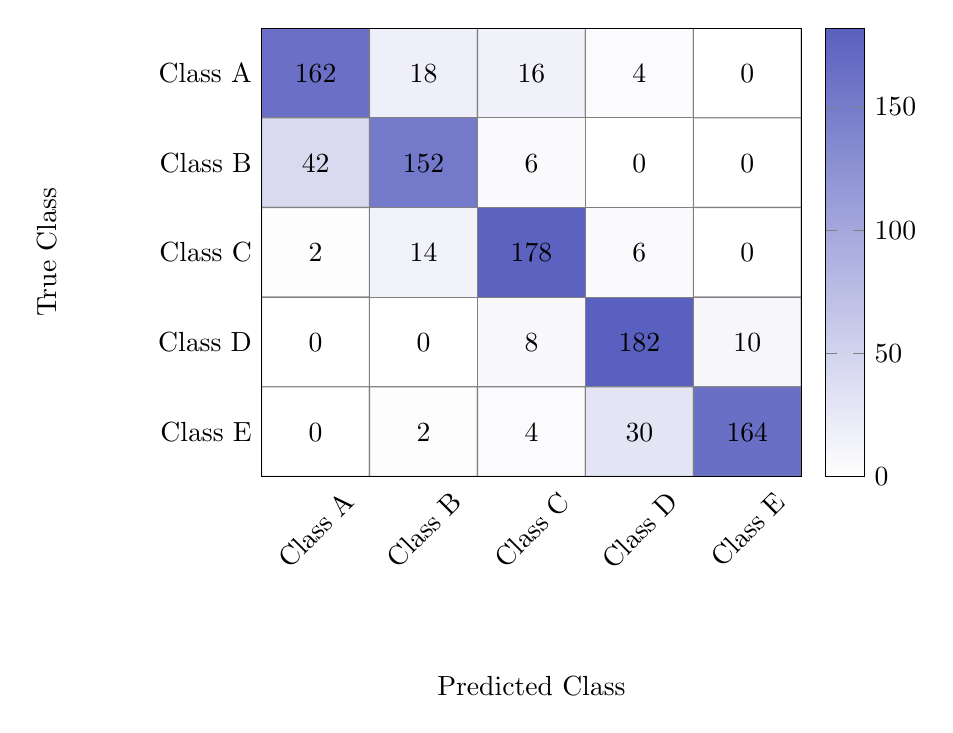
\begin{tikzpicture}
            \begin{axis}[
                    colormap={bluewhite}{color=(white) rgb255=(90,96,191)},
                    xlabel=Predicted Class,
                    xlabel style={yshift=-30pt},
                    ylabel=True Class,
                    ylabel style={yshift=30pt},
                    xticklabels={Class A, Class B, Class C, Class D, Class E},
                    xtick={0,...,4},
                    xtick style={draw=none},
                    yticklabels={Class A, Class B, Class C, Class D, Class E},
                    ytick={0,...,4},
                    ytick style={draw=none},
                    enlargelimits=false,
                    colorbar,
                    xticklabel style={
                      rotate=45
                    },
                    nodes near coords={\pgfmathprintnumber\pgfplotspointmeta},
                    nodes near coords style={
                        yshift=-7pt
                    },
                ]
                \addplot[
                    matrix plot,
                    mesh/cols=5,
                    point meta=explicit,draw=gray
                ] table [meta=C] {
                    x y C
                    0 0 162
                    1 0 18
                    2 0 16
                    3 0 4
                    4 0 0
                    
                    0 1 42
                    1 1 152
                    2 1 6
                    3 1 0
                    4 1 0
                    
                    0 2 2
                    1 2 14
                    2 2 178
                    3 2 6
                    4 2 0
            
                    0 3 0
                    1 3 0
                    2 3 8
                    3 3 182
                    4 3 10
            
                    0 4 0
                    1 4 2
                    2 4 4
                    3 4 30
                    4 4 164
                };
            \end{axis}
        \end{tikzpicture}
        \caption{Example of a good confusion matrix for a dataset with 200 samples per class. The sum of the values in each row $i$ must be equal to the number of samples in the dataset with true class $C_i$ (sum equal to 200 in this example). The accuracy of this model is $0.843$.}
    \end{figure}

    Sometimes, the values inside a confusion matrix are represented as percentages: each cell $c_{i,j}$ contains the ratio between the number of samples whose true class is $C_i$ and whose predicted class is $C_j$ over the total number of samples whose true class is $C_i$. In this case, the diagonal represents the \textit{accuracy} of the model for each class in $Y$.

    \begin{figure}[H]
        \centering
        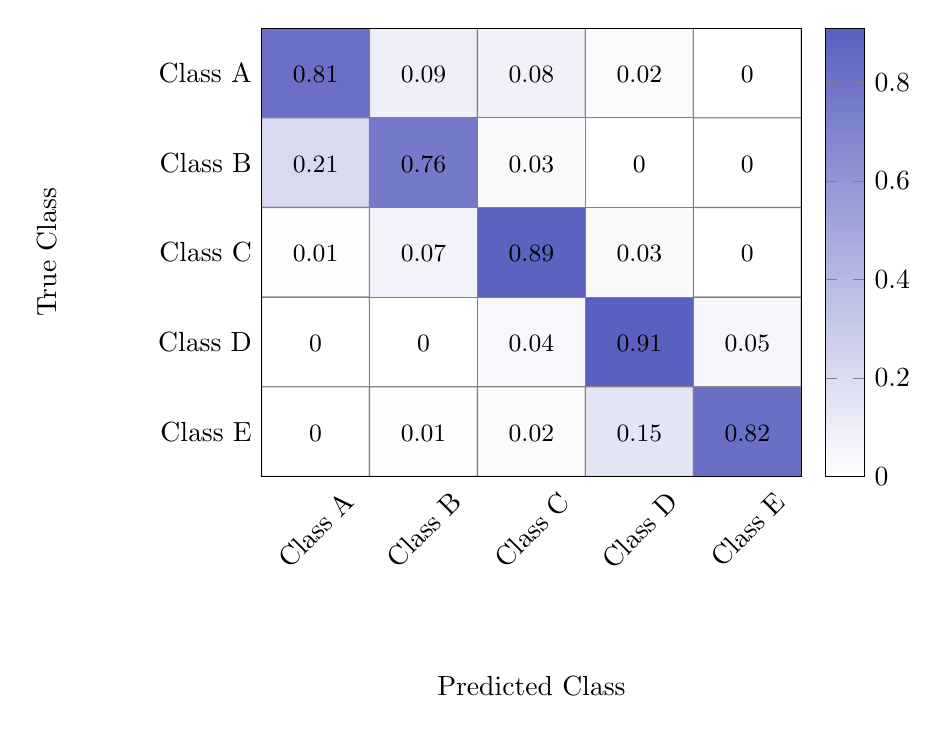
\begin{tikzpicture}
            \begin{axis}[
                    colormap={bluewhite}{color=(white) rgb255=(90,96,191)},
                    xlabel=Predicted Class,
                    xlabel style={yshift=-30pt},
                    ylabel=True Class,
                    ylabel style={yshift=30pt},
                    xticklabels={Class A, Class B, Class C, Class D, Class E},
                    xtick={0,...,4},
                    xtick style={draw=none},
                    yticklabels={Class A, Class B, Class C, Class D, Class E},
                    ytick={0,...,4},
                    ytick style={draw=none},
                    enlargelimits=false,
                    colorbar,
                    xticklabel style={
                      rotate=45
                    },
                    nodes near coords={\pgfmathprintnumber\pgfplotspointmeta},
                    nodes near coords style={
                        yshift=-7pt
                    },
                ]
                \addplot[
                    matrix plot,
                    mesh/cols=5,
                    point meta=explicit,
                    draw=gray,
                    nodes near coords style={
                        font=\small,
                        /pgf/number format/.cd,
                        fixed,
                        precision=3
                    },
                ] table [meta=C] {
                    x y C
                    0 0 0.81
                    1 0 0.09
                    2 0 0.08
                    3 0 0.02
                    4 0 0.00
                    
                    0 1 0.21
                    1 1 0.76
                    2 1 0.03
                    3 1 0.00
                    4 1 0.00
                    
                    0 2 0.01
                    1 2 0.07
                    2 2 0.89
                    3 2 0.03
                    4 2 0.00
            
                    0 3 0.00
                    1 3 0.00
                    2 3 0.04
                    3 3 0.91
                    4 3 0.05
            
                    0 4 0.00
                    1 4 0.01
                    2 4 0.02
                    3 4 0.15
                    4 4 0.82
                };
            \end{axis}
        \end{tikzpicture}
        \caption{Percentage representation of the previous confusion matrix. The sum of the values in each row must be equal to 1.}
    \end{figure}


    For regression problems $f : X \to \R^k$, we need a different type of metrics. In particular, given a test set $S = \{(x_i, t_i)\}_{i \in [N]}$, performance can be measured in various ways:
    \begin{itemize}
        \item \textbf{Mean Absolute Error (MAE)}
        \[\frac{1}{N} \sum_{i=1}^N \abs{\widehat{f}(x_i) - t_i} \]
        \item \textbf{Mean Squared Error (MSE)}
        \[\frac{1}{N} \sum_{i = 1}^N \abs{\widehat{f}(x_i) - t_i}^2\]
        \item \textbf{Root Mean Squared Error (RMSE)}
        \[\sqrt{\frac{1}{N} \sum_{i = 1}^N \abs{\widehat{f}(x_i) - t_i}^2}\]
    \end{itemize}

    where $\abs{\cdot}$ is the L2-norm operator. The K-Fold Cross Validation algorithm can also be adapted to compute these performance measures.

    \chapter{Decision trees}

    \section{Decision trees learning}

    After discussing the general idea behind machine learning problems and how to evaluate the solution retrieved by an algorithm, we're now ready to focus on how these algorithms work. In particular, we'll start by discussing decision trees.

    Given a discrete input space described by $m$ attributes $X = A_1 \times \ldots \times A_m$, where each $A_i$ is a finite set, and a problem $f : X \to Y$, a \textbf{decision tree} is a $n$-ary tree where:
    \begin{itemize}
        \item Each internal node is labeled by an attribute $A_i$
        \item Each branch outgoing from a node labeled with $A_i$ denotes a possible value of an attribute $v \in \mathrm{Values}(A_i)$, where the latter is the set of possible values for $A_i$
        \item Each leaf node of the tree is labeled with a class $j \in Y$
    \end{itemize}

    Given an input, a decision tree computes by querying the internal nodes (starting from the root) and always proceeds on the edge corresponding to the attribute value assumed by the input. In other words, a decision tree is nothing more than a set of rules that classifies any given input. Decision trees are a very easy computational model and they are capable of computing any discrete function. For example, suppose that we want to solve the concept learning problem $\mathrm{PlayTennis} : X \to \{\mathrm{Yes}, \mathrm{No}\}$ relative to deciding if good conditions are met in order to play tennis. The input set that we'll be working with is the following:
    \[X = \{\mathrm{Outlook} \times \mathrm{Temperature} \times \mathrm{Humidity} \times \mathrm{Wind}\}\]

    where:
    \[\mathrm{Outlook} = \{\mathrm{Sunny}, \mathrm{Overcast}, \mathrm{Rain}\} \qquad \mathrm{Temperature} = \{\mathrm{Hot}, \mathrm{Mild}, \mathrm{Cold}\}\]
    \[\mathrm{Humidity} = \{\mathrm{Normal}, \mathrm{High}\} \qquad\qquad\qquad \mathrm{Wind} = \{\mathrm{Weak}, \mathrm{Strong}\}\]

    \begin{figure}[H]
        \centering
        \begin{tabular}{cccccc}
            Day & Outlook & Temperature & Humidity & Wind & PlayTennis \\
            \hline
            D1 & Sunny & Hot & High & Weak & No \\
            D2 & Sunny & Hot & High & Strong & No \\
            D3 & Overcast & Hot & High & Weak & Yes \\
            D4 & Rain & Mild & High & Weak & Yes \\
            D5 & Rain & Cool & Normal & Weak & Yes \\
            D6 & Rain & Cool & Normal & Strong & No \\
            D7 & Overcast & Cool & Normal & Strong & Yes \\
            D8 & Sunny & Mild & High & Weak & No \\
            D9 & Sunny & Cool & Normal & Weak & Yes \\
            D10 & Rain & Mild & Normal & Weak & Yes \\
            D11 & Sunny & Mild & Normal & Strong & Yes \\
            D12 & Overcast & Mild & High & Strong & Yes \\
            D13 & Overcast & Hot & Normal & Weak & Yes \\
            D14 & Rain & Mild & High & Strong & No
        \end{tabular}
        \caption{Example dataset for \textit{PlayTennis}}
        \label{data_playtennis}
    \end{figure}

    A decision tree for this problem would look like the following:
    \begin{figure}[H]
        \centering

        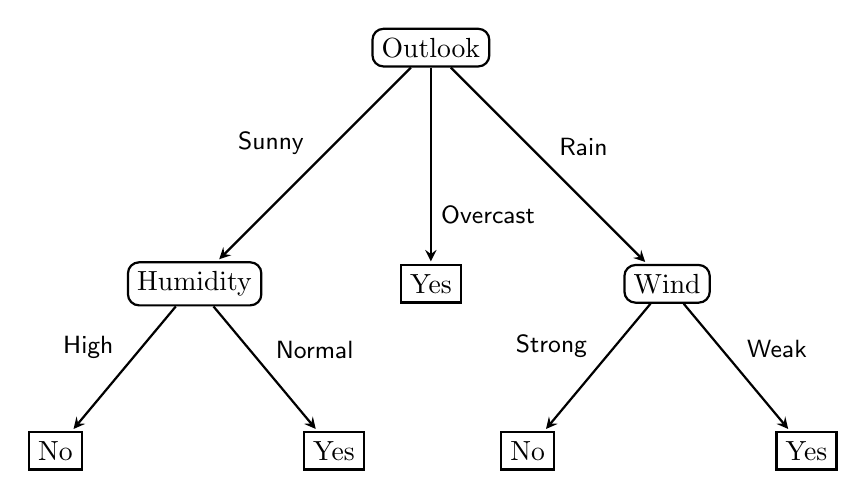
\begin{tikzpicture}[->,>=stealth,shorten >=1pt,auto,node distance=3cm, thick,main node/.style={scale=0.9,circle,draw,font=\sffamily\normalsize}]

            \node[rectangle, draw, rounded corners] (1)[] {$\mathrm{Outlook}$};

            \node[rectangle, draw] (2) [below of=1]{$\mathrm{Yes}$};
            \node[rectangle, draw, rounded corners] (3) [left of=2]{$\mathrm{Humidity}$};
            \node[rectangle, draw, rounded corners] (4) [right of=2]{$\mathrm{Wind}$};

            \node[rectangle, draw] (5) [below left of=3, xshift=10]{$\mathrm{No}$};
            \node[rectangle, draw] (6) [below right of=3, xshift=-10]{$\mathrm{Yes}$};
            \node[rectangle, draw] (7) [below left of=4, xshift=10]{$\mathrm{No}$};
            \node[rectangle, draw] (8) [below right of=4, xshift=-10]{$\mathrm{Yes}$};

            \path[every node/.style={font=\sffamily\small}]
                (1) edge[near end] node{Overcast} (2)
                (1) edge[swap] node{Sunny}(3)
                (1) edge node{Rain}(4)

                (3) edge[swap] node{High}(5)
                (3) edge node{Normal}(6)
                (4) edge[swap] node{Strong}(7)
                (4) edge node{Weak}(8)
                ;
        \end{tikzpicture}
        \caption{Example of decision tree for \textit{PlayTennis}.}
        \label{dt}
    \end{figure}

    In concept learning problems, each decision tree can be described as a disjunction of conjunction of the attributes tested by the tree. In particular, we consider only paths that end up with a positive leaf. For instance, the tree described above can also be represented as following:
    \[(\mathrm{Outlook = Sunny} \land \mathrm{Humidity = Normal})\]
    \[\lor (\mathrm{Outlook = Overcast}) \lor \]
    \[(\mathrm{Outlook = Rain} \land \mathrm{Wind = Weak})\]

    \subsection{Entropy and the ID3 algorithm}

    In this context, the hypothesis space is the \textit{set of all possible decision trees}. We'll now define the algorithm that we'll be using to derive an optimal decision tree from a given dataset: the \textbf{Iterative Dichotomiser 3 (ID3)} algorithm.

    \begin{framedalgo}[label={id3}]{ID3 algorithm}
        Given a dataset $D$ for a concept learning problem $f : X \to \{+,-\}$, an attribute list $L$ containing the attributes of $X$, the algorithm returns a decision tree for $f$.
        \begin{algorithmic}
            \Function{ID3}{$D,L$}
                \State Initialize an empty decision tree $T$
                \State Create a root node in $T$
                \If{All the examples in $D$ are positive}
                    \State{Label the root with $+$}
                \ElsIf{All the examples in $D$ are negative}
                    \State{Label the root with $-$}
                \ElsIf{$L = \varnothing$}
                    \State Label the root with the most common value for $A$ in $D$
                \Else
                    \State Let $A$ be the \textit{best decision attribute} in $L$ for $D$
                    \State Label the root with $A$
                    \For{$v \in \mathrm{Values}(A)$}
                        \State Let $D_a$ be the subset of $D$ whose tuples have $A$ set to $v$
                        \If{$D_a = \varnothing$}
                            \State Create a leaf node labeled with the most common value for $A$ in $D$
                            \State Add an edge labeled with $A = v$ from the root to the leaf node
                        \Else
                            \State Compute the subtree $T_A = \mathrm{ID3}(D_a, L-\{A\})$
                            \State Add an edge labeled with $A = v$ from the root to $T_A$
                        \EndIf
                    \EndFor
                    \EndIf
                \State Return $T$
            \EndFunction
        \end{algorithmic}
    \end{framedalgo}

    In the ID3 algorithm described above, the \textit{best decision attribute} is an attribute whose optimality depends on a pre-defined criteria. Based on the criteria chosen, different attributes may be selected. Trying to define an optimal criteria is crucial. In fact, based on the chosen attribute order, we may get a completely different decision tree.
    
    The commonly used measure for this task is the \textbf{information gain}, which measures how well a given attribute \textit{separates} the training examples according to their target classification. The information gain of an attribute is measured as reduction in \textbf{entropy}, which measures the impurity of a sample. 

    \begin{frameddefn}{Entropy}
        Let $S$ be a sample set for a classification problem $f : X \to Y$. For each $i \in Y$, we denote with $p_i$ the proportion of elements of $S$ that are classified as $C_i$. The \textbf{entropy} of $S$ is defined as:
        \[\mathrm{Entropy}(S) = - \sum_{i \in Y} p_i \log_2 p_i\]

        \textit{Note}: we assume that $0 \log_2 0 = 0$
    \end{frameddefn}

    In the special case of boolean classification problems -- since we have only two classes -- we denote with $p_{\oplus}$ and $p_{\ominus}$ the proportions of positive and negative samples in $S$ ($p_{\ominus} = 1-p_{\oplus})$. In this case, the entropy of $S$ is defined as:
    \[\mathrm{Entropy} = -p_\oplus \log_2 p_\oplus - p_\ominus \log_2 p_\ominus\]

    \begin{figure}[H]
        \centering
        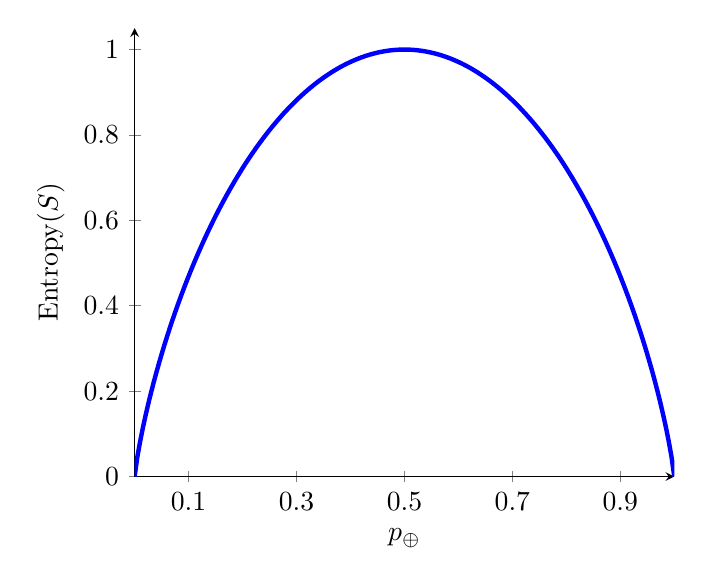
\begin{tikzpicture}
            \begin{axis}[
                xmax=1,ymax=1.05, samples=200, domain = 0:1,
                axis lines = left,
                xlabel = {$p_\oplus$},
                ylabel = {$\mathrm{Entropy}(S)$},
                xtick={0.1, 0.3, 0.5, 0.7, 0.9},
            ]

            \addplot[blue, ultra thick] {-x * log2(x) - (1-x) * log2(1-x)};
            \end{axis}
        \end{tikzpicture}
        \caption{The entropy function relative to a boolean classification}
    \end{figure}

    Through the graph above, it's easy to see that in boolean classification problems the entropy reaches its maximum value when $p_\oplus = 0.5$, i.e. when the two classes are perfectly balanced, while it reaches its minimum when $p_\oplus = 0$ or $p_\oplus = 1$. 

    \begin{frameddefn}{Information gain}
        The \textbf{information gain} for a sample set $S$ is defined as the expected reduction in entropy of $S$ caused by the selection of a value for the attribute $A$.
        \[\mathrm{Gain}(S,A) = \mathrm{Entropy}(S) - \sum_{v \in \mathrm{Values}(A)} \frac{\abs{S_v}}{\abs{S}} \; \mathrm{Entropy}(S_v)\]
        where $S_v = \{s \in S \mid A(s) = v\}$
    \end{frameddefn}

    Suppose that we have a sample set $S = [9+, 5-]$ (where this notation implies that we have 9 positives and 5 negatives) and that we are testing the information gain of the attribute $\mathrm{Wind} = \{\mathrm{Weak}, \mathrm{Strong}\}$. First, we compute the entropy of $S$:
    \[\mathrm{Entropy}(S) = -\frac{9}{14} \log_2 \rbk{\frac{9}{14}} - \frac{5}{14} \log_2 \rbk{\frac{5}{14}} \approx 0.940\] 
    
    After looking at the sample set, we get that $S_{\mathrm{Weak}} = [6+, 2-]$ and $S_{\mathrm{Strong}} = [3+, 3-]$. The entropy of these two subsets corresponds to:
    \[\mathrm{Entropy}(S_{\mathrm{Weak}}) = -\frac{6}{8} \log_2 \rbk{\frac{6}{8}} - \frac{2}{8} \log_2 \rbk{\frac{2}{8}} \approx 0.811\] 
    \[\mathrm{Entropy}(S_{\mathrm{Strong}}) = -\frac{3}{6} \log_2 \rbk{\frac{3}{6}} - \frac{3}{6} \log_2 \rbk{\frac{3}{6}} = 1\] 
    
    Hence, the information gain on $S$ knowing the attribute $\mathrm{Wind}$ corresponds to:
    \[\mathrm{Gain}(S,\mathrm{Wind}) = \mathrm{Entropy}(S) - \frac{8}{14} \mathrm{Entropy}(S_\mathrm{Weak}) - \frac{6}{14} \mathrm{Entropy}(S_\mathrm{Strng}) \approx 0.048\]

    Each time the ID3 algorithm has to select the best attribute, it always chooses the one with the highest information gain, corresponding to the one that most reduces the entropy. Eventually, the entropy of the \curlyquotes{implicitely partitioned} dataset will reach 1 or 0, meaning that the associated portion of the dataset contains only positive or negative values.

    Consider again the dataset $S$ shown in \Cref{data_playtennis}. This dataset contains 9 positive entries and 5 negative entries. First, the ID3 algorithm computes the information gain of all of the four attributes, finding that Outlook is the attribute that yields the highest gain.
    \begin{figure}[H]
        \centering
        \begin{tabular}{|c|c|c|c|}
            \hline
            Outlook & Temperature & Humidity & Wind \\
            \hline
            0.246 & 0.151 & 0.048 & 0.029 \\
            \hline
        \end{tabular}

        \caption{Gain on $S$ for each attribute}
    \end{figure}

    After setting Outlook as the root node, the algorithm now computes the three subtrees, one for each possible value of Outlook. Since the dataset $S_{\mathrm{Overcast}}$ contains only positive samples, the leaf node is labeled with Yes. The two other branches, instead, have to recursively compute their subtrees using information gain.

    \begin{figure}[H]
        \centering

        \resizebox{0.8\textwidth}{!}{
            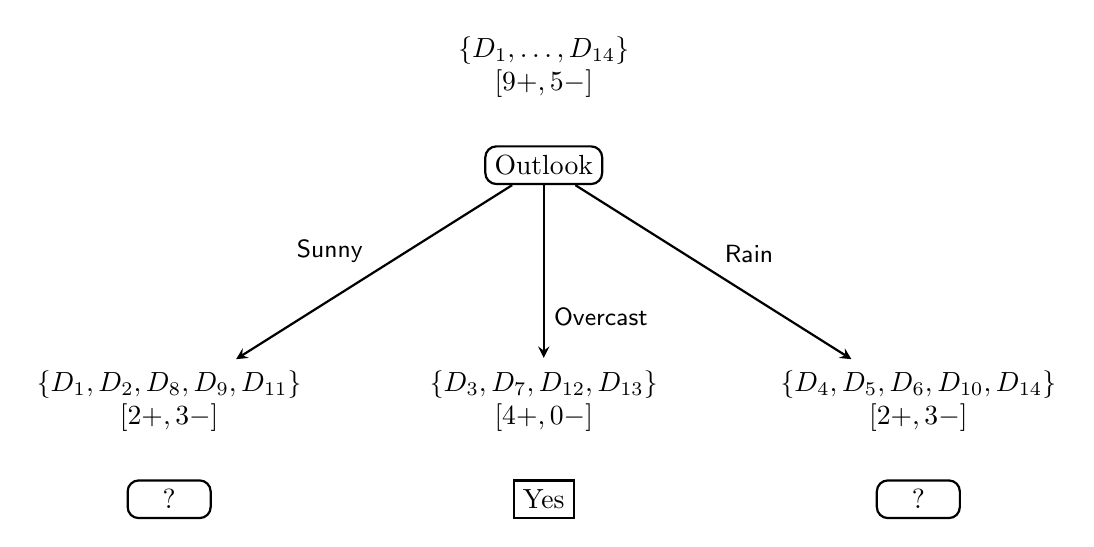
\begin{tikzpicture}[->,>=stealth,shorten >=1pt,auto,node distance=3cm, thick,main node/.style={scale=0.9,circle,draw,font=\sffamily\normalsize}]

                \node[] (1)[align = center] {$\{D_1, \ldots, D_{14}\}$ \\ $[9+, 5-]$};
                \node[rectangle, draw, rounded corners] (2)[below of = 1, yshift = 50] {$\mathrm{Outlook}$};
                
                \node[] (3)[below of = 2, align = center] {$\{D_3, D_7, D_{12}, D_{13}\}$ \\ $[4+, 0-]$};
                \node[rectangle, draw] (4)[below of = 3, yshift = 50] {$\mathrm{Yes}$};
                
                \node[] (5)[left of = 3, align = center, xshift=-50] {$\{D_1, D_2, D_{8}, D_{9}, D_{11}\}$ \\ $[2+, 3-]$};
                \node[rectangle, draw, rounded corners, minimum width=30] (6)[below of = 5, yshift = 50] {$\mathrm{?}$};

                \node[] (7)[right of = 3, align = center, xshift=50] {$\{D_4, D_5, D_{6}, D_{10}, D_{14}\}$ \\ $[2+, 3-]$};
                \node[rectangle, draw, rounded corners, minimum width=30] (8)[below of = 7, yshift = 50] {$\mathrm{?}$};

                \path[every node/.style={font=\sffamily\small}]
                    (2) edge[near end] node{Overcast} (3)
                    (2) edge[swap] node{Sunny} (5)
                    (2) edge[] node{Rain} (7)
                ;
            \end{tikzpicture}
        }
        \caption{The partially learned decision tree after the first level of recursion}
    \end{figure}

    After repeating the process for each level of recursion, we get the decision tree shown in \Cref{dt}. On each level of recursion, even though such hypothesis space is complete, meaning that every target function lies inside, the ID3 algorithm moves through such space in a greedy manner, returning only a \textbf{local minima}, while the target function is a \textbf{global minima}. Moreover, each step of the algorithm requires to analyze all the training examples, making this approach \textbf{not incremental} -- if we want to add more data, the whole tree must be recomputed. However, this also ensures that our statistically-based search choices are robust to noisy data.

    \subsection{Overfitting in decision trees}

    A common issue in decision tree learning is the \textbf{size} of the decision tree yield by the algorithm, that is the number of nodes in the output tree on average. The importance of size comes from the nature of the algorithm itself: since the hypothesis space is complete, if allow the tree to have an uge number of nodes then it will eventually become a perfect approximation of the dataset.

    \begin{figure}[H]
        \centering
        \includegraphics[scale=0.45]{images/overfitting_dt.png}
        \caption{Overfitting in decision trees}
    \end{figure}

    In the worst case, each entry of the dataset is a leaf of the decision tree. When this happens, the solution found by the algorithm is clearly overfitting the data. In decision tree learning, overfitting is \underline{unavoidable}. However, it can be reduced through some techniques. The first common technique involves enforcing a maximum growth on the tree by avoiding the recursive process when splitting the data wouldn't give a statistically significant improvement. The second technique grows the full decision tree and then prunes nodes that aren't significant. We'll focus on the second technique.

    To determine the optimal tree size, we use a separate set of examples (distinct from the training examples) to evaluate the utility of post-pruning, then apply a statistical test to estimate accuracy of a tree on the entire data distribution.

    In \textbf{reduced-error pruning}, the data is split into a training and a validation set.The easiest way to achieve each pruning step is to greedily select the subtree that is cut.
    \begin{enumerate}
        \item We copy the decision tree and randomly select a subtree
        \item We replace the whole subtree with a single leaf node labeled with the most common leaf label in the subtree.
        \item We test the accuracy on the new subtree through the validation set
    \end{enumerate}

    After evaluating the accuracy of every possible cut, we choose the one that increases the accuracy the most. Eventually, we'll reach a point where any additional cut will decrease the accuracy, concluding the pruning procedure.

    \begin{figure}[H]
        \centering
        \includegraphics[scale=0.45]{images/pruning_dt.png}
        \caption{Performance after reduced-error pruning.}
    \end{figure}

    One more successful method for finding high accuracy hypotheses is the \textbf{rule post-pruning} technique. Variants of this technique are used by C4.5, another decision tree learning algorithm.
    \begin{enumerate}
        \item We first infer the decision tree allowing it to overfit the dataset
        \item We convert the decision tree into an equivalent set of rules as shown in previous sections
        \item We generalize each rule as much as possible independently of others
        \item We remove multiple instances of the same generalized rule
        \item We sort the final set of rules into a desired sequence
        \item We convert the sequence back to a decision tree 
    \end{enumerate}

    Decision trees can also be used for classification of continuous-valued attributes. For instance, given the continuous-valued attribute Temperature, we can create a boolean variable that works with this attribute, such as \curlyquotes{Temperature > 72.3}. To work with such variables, the best approach is to pre-define the various splits of the set of continuous values.

    Moreover, decision trees can also use multi-valued attributes, such as dates. However, the information gain of these variables is usually too high. To relax this issue, one approach is to use the \textbf{Gain Ratio} instead of the gain.
    \[\mathrm{GainRatio}(S,A) = \frac{\mathrm{Gain}(S,A)}{\mathrm{SplitInformation}(S,A)}\]

    where $\mathrm{SplitInformation}(S,A) = - \sum_{i \in Y} \frac{\abs{S_i}}{\abs{S}} \log_2 \rbk{\frac{\abs{S_i}}{\abs{S}}}$ and $S_v = \{s \in S \mid A(s) = v\}$

    In some instances, we may want to give more importance to some particular attributes. To do so, we can define the \textbf{cost} for each attribute and replace the gain with one of the following values (they have no standard name)
    \[\frac{\mathrm{Gain}^2(S,A)}{\mathrm{Cost}(A)} \qquad\qquad \frac{2^{\mathrm{Gain}(S,A)}-1}{(\mathrm{Cost}(A)+1)^w} \;\; \text{for some $w \in [0,1]$}\]

    If some examples in the dataset have no value for the attribute selected by ID3, we can still use it through one of the following methods:
    \begin{enumerate}
        \item If node $u$ tests $A$, assign most common value of $A$ among other
        examples sorted to node $u$
        \item Assign most common value of $A$ among other examples with same
        target value
        \item Assign a probability $p_i$ to each possible value $v_i \in \mathrm{Value}(A)$, assigning fractions of $p_i$ to each descendant in tree
    \end{enumerate}

    \newpage

    \chapter{Probabilistic models}

    \section{Uncertainty and probability}

    When the problem that we want to learn is based on actions that may assume continuous values, defining a sequence discrete decision becomes hard. For instance, consider the action $A_t$ representing that Alice leaves for the airport $t$ minutes before her flight. In order to know which $t$ will satisfy the problem, we have to sort out many sub-problems, such as partial observability (road state, other drivers' plans, $\ldots$), noisy sensors (traffic reports), uncertainty in action outcomes (flat tire, $\ldots$), complexity of modelling and predicting traffic, $\ldots$.
    
    Hence an approach purely based on logical deduction will either risk falsehood, leads to conclusions that are too weak for decision making due to them requiring way too many conditions to be met (\curlyquotes{$A_{25}$ get me there on time if there's no accident on the bridge and it doesn't rain and my tires remain intact $\ldots$}) or may lead to non-optimal decisions that ensure the outcome (\curlyquotes{$A_{1440}$ will surely suffice, but I have to stay overnight in the airport}). When this is the case, the best option is to just accept \textbf{uncertainties} and find a way to work with them. In particular, this implies using a probabilistic approach.

    \begin{frameddefn}{Sample space and probability space}
        A \textbf{sample space} $\Omega$ is a set of finite or infinite outcomes. The elements $\omega \in \Omega$ are usually called \textit{atomic event} or \textit{outcome of a random process}.

        A \textbf{probability space} is a function $\Pr : \Omega \to [0,1]$ defined on a sample space where the sum of all the values equals 1
        \[\sum_{\omega \in \Omega} \Pr[\omega] = 1\]
    \end{frameddefn}

    Given a sample space $\Omega$, a probability space associates a probability in the range $[0,1]$ to each element of $\Omega$. Suppose that we want to model a probability space that represents the outcomes of a dice roll. The sample space can be defined as:
    \[\Omega = \{1,2,3,4,5,6\}\]

    If we're using a standard dice, the probability space will be defined as:
    \[\Pr[\omega] = \abk{\frac{1}{6}, \frac{1}{6}, \frac{1}{6}, \frac{1}{6}, \frac{1}{6}, \frac{1}{6}}\]

    If the dice is loaded, instead, some outcomes may be more-likely. For instance, we could have the following probability space:
    \[\Pr[\omega] = \abk{\frac{1}{2}, 0, \frac{1}{6}, 0, \frac{1}{6}, \frac{1}{6}}\]

    \begin{frameddefn}{Event}
        Given a probability space $\Pr : \Omega \to [0,1]$, an \textbf{event} is a subset of $\Omega$. The probability of an event $A \subseteq \Omega$ is given by the sum of the probabilities of all of the outcomes in the event.
        \[\Pr[A] = \sum_{\omega \in A} \Pr[\omega]\]
    \end{frameddefn}

    Using the previous loaded dice example, the event \curlyquotes{roll a value lower than 4} is described by the event $A = \{1,2,3\}$ and its probability is $\Pr[A] = \frac{5}{6}$. Events are a simple way to reason about probability. However, sometimes they aren't as intuitive as they look. For this reason, we usually prefer to work with \textit{random variables}.

    \begin{frameddefn}{Random variable}
        Given a probability space $\Pr : \Omega \to [0,1]$, a \textbf{random variable} is a function $X : \Omega \to B$, where $B$ is an arbitrary set of values.
    \end{frameddefn}

    A random variable associates one of the values in $B$ to every single element of the sample space. To work with a random variable $X : \Omega \to B$, we often consider the event \curlyquotes{$X = x_i$}, where $x_i \in B$. This event is equivalent to the set $\{\omega \in \Omega \mid X(\omega) = x_i\}$. Due to this, a random variable can be viewed both as a function and a variable.
    \[\Pr[X = x_i] = \Pr[\{\omega \in \Omega \mid X(\omega) = x_i\}] = \sum_{\substack{\omega \in \Omega \; :\\ X(\omega) = x_i}} \Pr[\omega]\]

    When we're working with a boolean random variable, i.e. when the value set $B$ is $\{0,1\}$, we often denote the event \curlyquotes{$X = 1$} with $X$, while the event \curlyquotes{$X = 1$} is denoted with $\lnot X$. This allows us to write intersections and unions of events as simple conjunctions and disjunctions of boolean random variables.
    \[\Pr[\lnot A \land B] = \sum_{\substack{\omega \in \Omega \;:\\ A(\omega) = 0, B(\omega) = 1}} \Pr[\omega]\]

    Instead of working with a probability space in order to compute the probabilities of each value assumable by a random variable, we often directly consider a \textbf{probability distribution}, a function assigning a probability value to all possible assignments of a random variable. The \textit{joint probability distribution} for a set of random variables gives the probability of every atomic joint event on those random variables.
    \begin{figure}[H]
        \centering
        \begin{tabular}{cc|cccc}
            \multicolumn{2}{c}{$\Pr[\mathrm{PlayTennis} \land \mathrm{Weather}]$} & \multicolumn{4}{c}{Weather} \\
            & & Sunny & Rainy & Cloudy & Snowy \\
            \cline{2-6}
            \multirow{2}{*}{PlayTennis} & True & $0.576$ & $0.02$ & $0.064$ & $0.01$ \\
            & False &$0.144 $ & $0.08 $ & $0.016 $ & $0.09$
        \end{tabular}
        \caption{Example of joint probability distribution}
    \end{figure}

    We notice that, by definition, the probability of the conjunction of two events is not always equal to the product of the two probabilities of the events.
    \[\Pr[A \land B] \stackrel{?}{=} \Pr[A] \cdot \Pr[B]\]
    
    When the equality holds, we say that the two events are \textbf{independent} from each other. For the probability of the disjunction of two events, instead, we can always use the following formula derived from the \textit{inclusion-exclusion principle}:
    \[\Pr[A \lor B] = \Pr[A] + \Pr[B] - \Pr[A \land B]\]

    Random variables can also influence each others. For instance, if we know that some outcomes of an event $A$ are more likely to happen when some conditions are met, we can restrict our interest to such cases. The probability of an event $A$ given that an event $B$ happened is written $\Pr[A \mid B]$. This is also known as \textbf{conditional} (or \textit{posterior}) probability and its defined as:
    \[\Pr[A \mid B] = \frac{\Pr[A, B]}{\Pr[B]}\]
    
    where $\Pr[A, B] = \Pr[A \land B]$. We notice that the events $A$ and $B$ are independent if and only if $\Pr[A \mid B] = \Pr[A]$. Sometimes, we may be also be given \textit{conditional probability distributions}.
    \begin{figure}[H]
        \centering
        \begin{tabular}{cc|cccc}
            \multicolumn{2}{c}{$\Pr[\mathrm{PlayTennis} \mid \mathrm{Weather}]$} & \multicolumn{4}{c}{Weather} \\
            & & Sunny & Rainy & Cloudy & Snowy \\
            \cline{2-6}
            \multirow{2}{*}{PlayTennis} & True & $0.8$ & $0.2$ & $0.8$ & $0.1$ \\
            & False &$0.2 $ & $0.8 $ & $0.2 $ & $0.9$
        \end{tabular}
        \caption{Example of conditional probability distribution}
    \end{figure}

    When this is the case, conditional probability can be used to compute joint probability. This is also known as the \textit{product rule}.
    \[\Pr[A , B] = \Pr[A \mid B] \cdot \Pr[B]\]

    When the values of a random variable $Y$ are \underline{mutually exclusive}, we may compute the total probability of another random variable $X$ through joint probability or conditional probability. This is called \textbf{total probability}.
    \[\begin{split}
        \Pr[X = x] & = \Pr[(X = x , Y = y_1) \lor \ldots \lor (X = X , Y = y_k)] \\
        & = \sum_{i = 1}^k \Pr[X = x , Y = y_i] \\
        & = \sum_{i = 1}^k \Pr[X = x \mid Y = y_i] \cdot \Pr[Y = y_i] \\
    \end{split}\]

    Conditional probability can clearly be viewed as a \textbf{normalization factor} $\alpha$ applied to a joint probability. For instance, given the conditional probability, we have that:
    \[\Pr[A \mid B] = \frac{\Pr[A , B]}{\Pr[B]} = \alpha \Pr[A , B]\]
    where the normalization factor is $\alpha = \frac{1}{\Pr[B]}$. Viewing such probability as nothing more than a normalized instance of the joint one allows us to reason about maximizing and minimizing values in a simpler way: since each element is afflicted by this constant factor, we can just ignore. 
    \[\argmax_{x \in \mathrm{Values}(X)} \Pr[X = x \mid Y = y] = \argmax_{x \in \mathrm{Values}(X)} \alpha \Pr[X = x , Y = y] = \argmax_{x \in \mathrm{Values}(X)} \Pr[X = x, Y = y]\]

    The most important rule derived from the very definition of conditional probability is \textbf{Bayes' rule}. This rule allows us to invert the order of the events: to compute the probability of $A$ given $B$, we can use the probability of $B$ given $A$

    \begin{framedprop}{Bayes' rule}
        Given two events $A$ and $B$, it holds that:
        \[\Pr[A \mid B] = \frac{\Pr[B \mid A] \cdot \Pr[A]}{\Pr[B]}\]
    \end{framedprop}

    Bayes' rule becomes even stronger in the context of maximizing and minimizing values thanks to normalization:
    \[\argmax_{x \in \mathrm{Values}(X)} \Pr[X = x \mid Y = y] = \argmax_{x \in \mathrm{Values}(X)} \Pr[Y = y \mid X = x] \cdot \Pr[X = x]\]
    
    Moreover, when the conditions $Y_1, \ldots, Y_k$ are independent from each other, we also get that:
    \[\Pr[X \mid Y_1, \ldots, Y_k] = \alpha \Pr[Y_1, \ldots, Y_k \mid X] \cdot \Pr[X] = \alpha \Pr[Y_1 \mid X] \cdot \ldots \cdot \Pr[Y_k \mid X] \cdot \Pr[X]\]

    Another interesting consequence of the product rule is the \textit{chain rule}, where we repeatedly apply the product rule on each joint probability:
    \[\begin{split}
        \Pr[X_1, \ldots, X_{n-1}, X_n] & = \Pr[X_1, \ldots, X_{n-1}] \cdot \Pr[X_n \mid X_1, \ldots, X_{n-1}] \\
        & = \Pr[X_1, \ldots, X_{n-2}] \cdot \Pr[X_{n-1} \mid X_1, \ldots, X_{n-2}] \cdot \Pr[X_n \mid X_1, \ldots, X_{n-1}] \\
        &= \prod_{i = 1}^n \Pr[X_i \mid X_1, \ldots, X_{i-1}]
    \end{split}\]

    The chain rule is usually used with \textbf{Bayesian networks}, a graphical notation for conditional independence assertions and hence for compact specification of full joint distributions.

    Given a set of variables, a Bayesian networks is a directed acyclic graph containing one node for each variable. The directed edges of the graph describe influences between variables: an edge $(Y,X)$ implies that $Y$ influences $X$. Each influence $(Y,X)$ is associated with a conditional probability $\Pr[X \mid Y]$. In the simplest case, the conditional distribution is represented as a \textbf{Conditional Probability Table (CPT)} giving the distribution over $X$ for each combination of its parent values.

    For instance, consider the following situation. Suppose, that while we're working, our neighbor John calls to say that our alarm is ringing, but our other neighbor Mary doesn't call. However, we know that the alarm can be set off by minor earthquakes. Can we use probabilities to decide if there is a burglar?

    First, we define five variables: Burglar, Earthquake, Alarm, JohnCalls, MaryCalls. Then, we consider the relations between such variables based on what we know:
    \begin{itemize}
        \item A burglar can set the alarm, hence $\mathrm{Burglar} \in \mathrm{Parent(Alarm)}$
        \item An earthquake can set the alarm, hence $\mathrm{Earthquake} \in \mathrm{Parent(Alarm)}$
        \item The alarm can cause John to call, hence $\mathrm{Alarm} \in \mathrm{Parent(JohnCalls)}$
        \item The alarm can cause Mary to call, hence $\mathrm{Alarm} \in \mathrm{Parent(MaryCalls)}$
    \end{itemize}

    \begin{figure}[H]
        \centering

        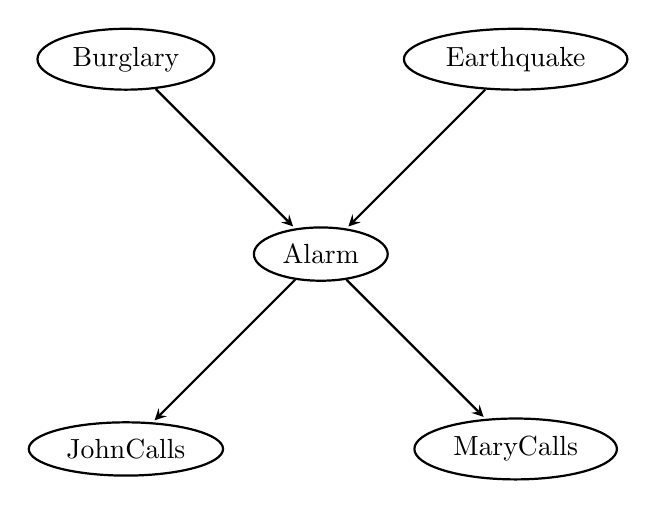
\begin{tikzpicture}[->,>=stealth,shorten >=1pt,auto,node distance=3.5cm, thick,main node/.style={scale=0.9,circle,draw,font=\sffamily\normalsize}]
            \usetikzlibrary{shapes.geometric}

            \node[ellipse, draw] (1)[] {Alarm};
            \node[ellipse, draw] (2)[above left of = 1] {Burglary};
            \node[ellipse, draw] (3)[above right of = 1] {Earthquake};
            \node[ellipse, draw] (4)[below left of = 1] {JohnCalls};
            \node[ellipse, draw] (5)[below right of = 1] {MaryCalls};

            \path[every node/.style={font=\sffamily\small}]
                (2) edge (1)
                (3) edge (1)
                (1) edge (4)
                (1) edge (5)
            ;
        \end{tikzpicture}
        \caption{The Bayesian network representing the \textit{BurlaryProblem}}
    \end{figure}

    For each variable, we construct a CPT representing the conditional probabilities for each of the parent attributes.

    \begin{figure}[H]
        \centering

        \resizebox{1\textwidth}{!}{
            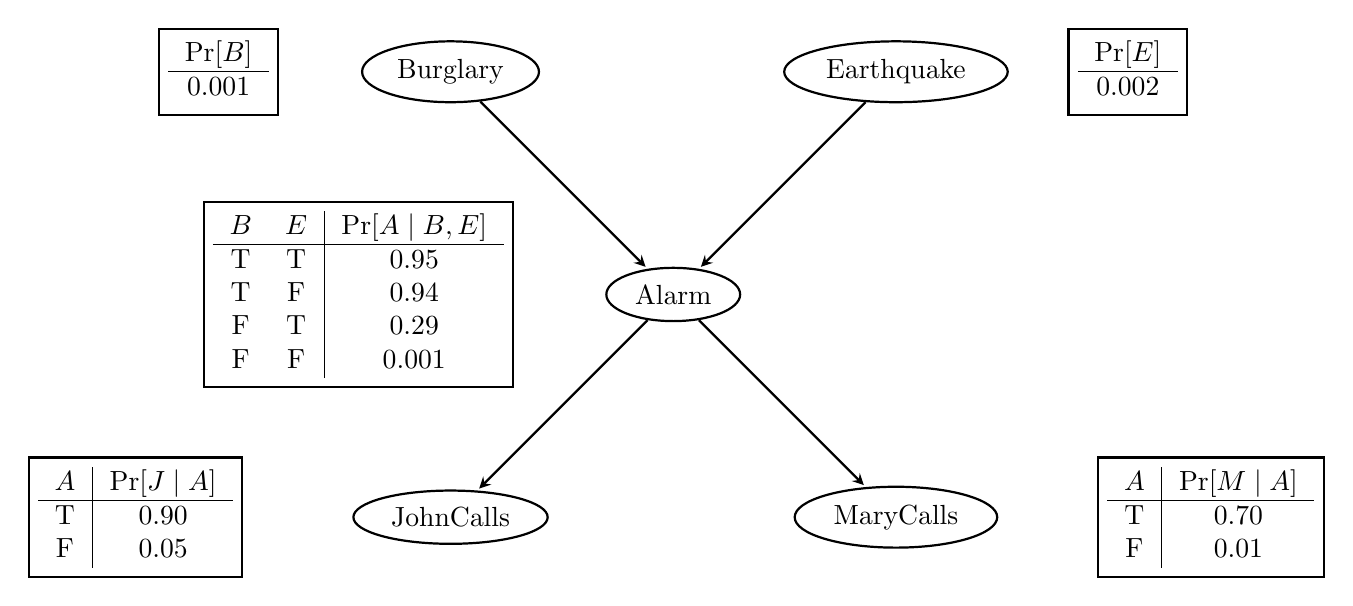
\begin{tikzpicture}[->,>=stealth,shorten >=1pt,auto,node distance=4cm, thick,main node/.style={scale=0.9,circle,draw,font=\sffamily\normalsize}]
                \usetikzlibrary{shapes.geometric}

                \node[ellipse, draw] (1)[] {Alarm};
                \node[ellipse, draw] (2)[above left of = 1] {Burglary};
                \node[ellipse, draw] (3)[above right of = 1] {Earthquake};
                \node[ellipse, draw] (4)[below left of = 1] {JohnCalls};
                \node[ellipse, draw] (5)[below right of = 1] {MaryCalls};

                \node[rectangle, draw] (6) [left of = 2, xshift=30] {\begin{tabular}{c}
                    $\Pr[B]$ \\
                    \hline 
                    $0.001$
                \end{tabular}};

                \node[rectangle, draw] (7) [right of = 3, xshift =-30] {\begin{tabular}{c}
                    $\Pr[E]$ \\
                    \hline
                    $0.002$
                \end{tabular}};

                \node[rectangle, draw] (8) [left of = 1] {\begin{tabular}{cc|c}
                    $B$ & $E$ & $\Pr[A \mid B, E]$ \\
                    \hline
                    T & T & $0.95$ \\
                    T & F & $0.94$ \\
                    F & T & $0.29$ \\
                    F & F & $0.001$ \\
                \end{tabular}};

                \node[rectangle, draw] (8) [left of = 4] {\begin{tabular}{c|c}
                    $A$ & $\Pr[J \mid A]$ \\
                    \hline
                    T & $0.90$ \\
                    F & $0.05$ \\
                \end{tabular}};
                \node[rectangle, draw] (8) [right of = 5] {\begin{tabular}{c|c}
                    $A$ & $\Pr[M \mid A]$ \\
                    \hline
                    T & $0.70$ \\
                    F & $0.01$ \\
                \end{tabular}};

                \path[every node/.style={font=\sffamily\small}]
                    (2) edge (1)
                    (3) edge (1)
                    (1) edge (4)
                    (1) edge (5)
                ;
            \end{tikzpicture}
        }
        \caption{The Bayesian network representing the \textit{BurlaryProblem}}
    \end{figure}

    Using the chain rule, the probability that both Mary and John call when the alarm rings while there is no burlar or earthquake is given by:
    \[\Pr[\mathrm{\lnot B, \lnot E, A, J, M}] = \Pr[\lnot B] \cdot \Pr[\lnot E] \cdot \Pr[A \mid \lnot B, \lnot E] \cdot \Pr[J \mid A] \cdot \Pr[M \mid A] \approx 0.00063\]
    
    \section{Bayesian learning}
    
    \subsection{Optimal Bayes classifier}

    In classification problems, Bayesian learning provides practical learning algorithms based on multiple parameters, combining prior knowledge (in particular prior probabilities) with new observed data, making probabilistic decisions.

    Given a dataset and an instance $x \in X$, the latter gets classified with the most probable class for that instance and that dataset. In other words, given a classification problem $f : X \to Y$, a dataset $D$ and a new instance $x \in X$, the best class prediction $C^* \in Y$ for $x$ over $D$ is given by:
    \[C^* \in \argmax_{C \in Y} \Pr[C \mid x, D]\]

    Similarly, learning is also achieved through probability. Given dataset $D$ and hypothesis space $H$, we're interested in the hypothesis $h^* \in H$ that maximizes the probability for the given dataset.
    \[h^* \in \argmax_{h \in H} \Pr[h \mid D]\]

    As the name suggests, Bayesian learning is based on Bayes' rule. In general, we're interested in two types of hypotheses: the \textit{maximum a posteriori} hypothesis and the \textit{maximum likelihood} hypothesis. The former is achieved by applying Bayes' rule, inverting the order of the events:
    \[\begin{split}
        h_{\mathrm{MAP}} \in \argmax_{h \in H} \Pr[h \mid D] = \argmax_{h \in H} \Pr[D \mid h] \cdot \Pr[h]\\
    \end{split}\]

    The latter, instead, also assumes that the hypotheses are \textbf{uniformly distributed}, i.e. that they all have the same probability. In this case, since $\Pr[h_i] = \Pr[h_j]$ for all $h_i,h_j \in H$, we can ignore this probability:
    \[h_{\mathrm{ML}} \in \argmax_{h \in H} \Pr[h \mid D] = \argmax_{h \in H} \Pr[D \mid h] \cdot \Pr[h] = \argmax_{h \in H} \Pr[D \mid h]\]

    \begin{frameddefn}{MAP and ML hypotheses}
        Given a classification problem $f : X \to Y$ and a dataset $D$, the \textbf{maximum a posteriori (MAP)} hypothesis $h_{\mathrm{MAP}}$ and the  \textbf{maximum likelihood (ML)} hypothesis $h_{\mathrm{ML}}$ are defined as:
        \[h_{\mathrm{MAP}} \in \argmax_{h \in H} \Pr[D \mid h] \cdot \Pr[h]\]
        \[h_{\mathrm{ML}} \in \argmax_{h \in H} \Pr[D \mid h]\]
\end{frameddefn}

    By definition, $h_{\mathrm{MAP}}^*$ and $h_{\mathrm{ML}}^*$ are two types of optimal hypotheses for a \textit{given} dataset $D$. Hence, for any instance $x \in X$, the classes $h^*_{\mathrm{MAP}}(x)$ and $h^*_{\mathrm{MAP}}(x)$ may not be the most probable classification for $x$ in \textit{general}, meaning that we don't care about the specific dataset. For instance, suppose we have three hypotheses $h_1, h_2, h_3$ for a dataset $D$, where:
    \[\Pr[h_1 \mid D] = 0.4 \qquad \Pr[h_2 \mid D] = 0.3 \qquad \Pr[h_3 \mid D] = 0.3\]
    
    Given an instance $x \in X$, suppose that:
    \[h_1(x) = \oplus \qquad h_2(x) = \ominus \qquad h_3(x) = \ominus\]

    Here, for both MAP and ML hypotheses, the most probable hypothesis is clearly $h_1$. Hence, we would classify $x$ as type $\oplus$. However, the most probable class for $x$ in general is clearly $\ominus$. To fix this issue, we can use the \textbf{Optimal Bayes Classifier} method, which is based on total probability. Given an instance $x \in X$ and a class $C \in Y$ with a dataset $D$, we have that:
    \[\Pr[C \mid x, D] = \sum_{h \in H} \Pr[C \mid x,h,D] \cdot \Pr[h \mid x,D] = \sum_{h \in H} \Pr[C \mid x,h] \cdot \Pr[h \mid D]\]

    The last equivalence is given by the fact that:
    \begin{itemize}
        \item When $h$ is fixed, the probability that $h(x) = C$ is independent from $D$, hence $\Pr[C \mid x,h,D] = \Pr[C \mid x,h]$
        \item $h$ is always independent from $x$, hence $\Pr[h \mid x,D] = \Pr[h \mid D]$
    \end{itemize}
    
    \begin{frameddefn}{Optimal Bayes Classifier}
        Given a classification problem $f : X \to Y$, a dataset $D$ and a new instance $x \in X-X_D$, the Optimal Bayes Classification for $x$ over $D$ is given by:
        \[C_{\mathrm{OB}} \in \argmax_{C \in Y} \sum_{h \in H} \Pr[C \mid x, h] \cdot \Pr[h \mid D]\]
    \end{frameddefn}

    As the name suggests, this method is an \textbf{optimal learner}, meaning that no other classification method using the same hypothesis space and same prior knowledge can outperform this method on average. This method maximizes the probability that the new instance $x$ is classified correctly. For instance, consider again the previous example. We have that:
    \[\begin{array}{ccccc}
        \Pr[h_1 \mid D] = 0.4 & \qquad\qquad & \Pr[h_2 \mid D] = 0.3 & \qquad\qquad & \Pr[h_3 \mid D] = 0.3 \\
        \Pr[\oplus \mid x, h_1] = 1 & & \Pr[\oplus \mid x, h_2] = 0 & & \Pr[\oplus \mid x, h_3] = 0  \\
        \Pr[\ominus \mid x, h_1] = 0 & & \Pr[\ominus \mid x, h_2] = 1 & & \Pr[\ominus \mid x, h_3] = 1  \\
    \end{array}\]

    We notice that:
    \[\sum_{h_i \in H} \Pr[\oplus \mid x, h_i] \cdot \Pr[h_i \mid D] = 0.4 \qquad\qquad \sum_{h_i \in H} \Pr[\ominus \mid x, h_i] \cdot \Pr[h_i \mid D] = 0.6\]

    Hence, the Optimal Bayes Classifier would correctly label the instance $x$ with $\ominus$. To get the full picture behind the power of this optimal learner, we consider a more complex example.

    Suppose that we have four kinds of candy bags:
    \begin{enumerate}
        \item The first type contains only candies with the cherry flavor
        \item The second type contains $75\%$ of cherry candies and $25\%$ of lime candies
        \item The third type contains $50\%$ of cherry candies and $50\%$ of lime candies
        \item The fourth type contains $25\%$ of cherry candies and $75\%$ of lime candies
        \item The fifth type contains only candies with the lime flavor
    \end{enumerate}

    A box containing bags of candies arrives to our shop. We know that:
    \begin{enumerate}
        \item $10\%$ of the bags are of the first flavor
        \item $20\%$ of the bags are of the second flavor
        \item $40\%$ of the bags are of the third flavor
        \item $20\%$ of the bags are of the fourth flavor
        \item $10\%$ of the bags are of the fifth flavor
    \end{enumerate}

    We choose a random bag from the box -- without knowing its type -- and extract some candies from it. We want to learn which type of bag we picked and what is the probability of extracting a candy of a specific flavor next.

    First, we model our distribution prior probabilities for the hypothesis space. Each type of bag corresponds to a hypothesis, meaning that:
    \[\Pr[H] = \abk{\frac{1}{10}, \;\; \frac{1}{5}, \;\; \frac{2}{5}, \;\; \frac{1}{5}, \;\; \frac{1}{10}}\]

    The distribution for extracting a lime candy for each hypothesis is given by:
    \[\Pr[\ell \mid H] = \abk{0, \;\; \frac{1}{4}, \;\; \frac{1}{2}, \;\; \frac{3}{4}, \;\; 1}\]
    
    Since we haven't extracted any candy, our previous knowledge is none -- hence, the dataset is empty. The probability of the first candy having lime flavor in this case is given by:
    \[\Pr[\ell \mid x_1] = \sum_{h_i \in H} \Pr[\ell \mid x, h_i] \cdot \Pr[h_i] = 0 \cdot \frac{1}{10} + \frac{1}{4} \cdot \frac{1}{5} + \frac{1}{2} \cdot \frac{2}{5} + \frac{3}{4} \cdot \frac{1}{5} + 1 \cdot \frac{1}{10} = \frac{1}{2}\]

    Suppose that the first candy is indeed a lime candy. For the following extraction, our dataset will be $D_1 = \{(x_1, \ell)\}$. Through Bayes' rule, we have that:
    \[\Pr[H \mid D_1] = \frac{\Pr[D_1 \mid H] \cdot \Pr[H]}{\Pr[D_1]} = 2 \Pr[D_1 \mid H] \cdot \Pr[H] = 2 \Pr[\ell \mid H] \cdot \Pr[H]\]

    Hence, we have that:
    \[\Pr[H \mid D_1] =  2 \cdot \abk{0 \cdot \frac{1}{10}, \;\; \frac{1}{4} \cdot \frac{1}{5}, \;\; \frac{1}{2} \cdot \frac{2}{5}, \;\; \frac{3}{4} \cdot \frac{1}{5}, \;\; 1 \cdot \frac{1}{10}} = \abk{0, \;\; \frac{1}{10}, \;\; \frac{2}{5}, \;\; \frac{3}{10}, \;\; \frac{1}{5}} \]

    The probability of extracting a second lime candy is given by:
    \[\Pr[\ell \mid x_2, D_1] = \sum_{h_i \in H} \Pr[\ell \mid x_2, h_i] \cdot \Pr[h_i \mid D_1] = 0 \cdot 0 + \frac{1}{4} \cdot \frac{1}{10} + \frac{1}{2} \cdot \frac{2}{5} + \frac{3}{4} \cdot \frac{3}{10} + 1 \cdot \frac{1}{5} = \frac{13}{20}\]

    Suppose that we extract another lime candy. The dataset is now $D_2 = \{(x_2, \ell), (x_1, \ell)\}$.
    \[\Pr[H \mid D_2] = \frac{\Pr[D_2 \mid H] \cdot \Pr[H]}{\Pr[D_2]} = \frac{20}{13} \Pr[D_2 \mid H] \cdot \Pr[H]\]

    Since the data samples in $D_2$ are independent from each other, we have that:
    \[\Pr[H \mid D_2] = \frac{20}{13} \Pr[\{(x_2, \ell)\} \mid H] \cdot \Pr[\{(x_1, \ell)\} \mid H] \cdot \Pr[H] = \frac{20}{13} \Pr[\ell \mid H] \cdot \Pr[H \mid D_1]\]

    Again, we now have that:
    \[\Pr[H \mid D_2] =  \frac{20}{13} \cdot \abk{0 \cdot 0, \;\; \frac{1}{4} \cdot \frac{1}{10}, \;\; \frac{1}{2} \cdot \frac{2}{5}, \;\; \frac{3}{4} \cdot \frac{3}{10}, \;\; 1 \cdot \frac{1}{5}} = \abk{0, \;\; \frac{1}{26}, \;\; \frac{4}{13}, \;\; \frac{9}{26}, \;\; \frac{4}{13}} \]

    If we keep extracting a lime candy, the posterior probability of the fifth hypothesis will skyrocket. Using the MAP hypothesis, the fifth one will be selected. However, the selected hypothesis may not be the correct one: the fifth hypothesis clearly overfits our dataset.

    \begin{figure}[H]
        \centering
        \includegraphics[scale=0.5]{images/bayesian_ex1.png}
        \caption{Probability of the five hypotheses with the increase in the number of samples}
    \end{figure}

    Consider now a new manufacturer producing bags with an arbitrary choice of cherry/lime candies. Let $\theta \in [0,1]$ be the ratio of cherry candies over all the $N$ candies, i.e. $\theta = \frac{\text{num. of cherry candies}}{N}$. For each possible $\theta$, we consider the hypothesis $h_\theta$, where:
    \[\Pr[c \mid h_\theta] = \theta \qquad\qquad \Pr[\ell \mid h_\theta] = 1-\theta\]
    
    This implies that we have a continuous hypothesis space. The dataset is given by the number of cherry samples $c$ and lime samples $\ell$, where $N = c + \ell$. We want to find the ML hypothesis of this setup.
    \[h^*_{\mathrm{ML}} \in \argmax_{\theta \in [0,1]} \Pr[D \mid h_\theta]\]

    We notice that:
    \[\Pr[D \mid h_\theta] = \prod_{i = 1}^N \Pr[d_i \mid h_\theta] = \theta^c \cdot (1-\theta)^\ell\]
    where $d_i \in D$. Hence, we get that:
    \[h_{\theta_\mathrm{ML}} \in \argmax_{\theta \in [0,1]} \Pr[D \mid h_\theta] = \theta^c \cdot (1-\theta)^\ell\]

    To get an even better result, we can use the properties of logarithms:
    \[h_{\mathrm{ML}} \in \argmax_{\theta \in [0,1]} \theta^c \cdot (1-\theta)^\ell = \argmax_{\theta \in [0,1]} \log (\theta^c \cdot (1-\theta)^\ell) = \argmax_{\theta \in [0,1]} c \log \theta + \ell \log (1-\theta)\]

    Since we're working with the continuous interval $[0,1]$, to find the value $\theta^* \in [0,1]$ that maximizes the probability we can use derivatives:
    \[\frac{d L(D \mid h_\theta)}{d \theta} = \frac{c}{\theta} - \frac{\ell}{1-\theta} \implies \frac{c}{\theta} - \frac{\ell}{1-\theta} = 0 \implies \theta_{ML} = \frac{c}{c+\ell} = \frac{c}{N}\]
    concluding that the value $\theta_{ML}$ which gives the best hypothesis $h_{\mathrm{ML}}$ is the one representing the ratio of cherry candies in the dataset -- as anyone would expect.

    In general, given a dataset $D$ where for each $d_i \in D$ we have that $d_i \in \{0, 1\}$, assuming a probability distribution for $D$ over an interval $\Theta$, the maximum likelihood estimation is given by:
    \[\theta_{ML} \in \argmax_{\theta \in \Theta} \log \Pr[d_i \mid h_\theta]\]

    In the particular case of Bernoulli distributions, i.e. where the variable $X$ represents the number of extractions of positive type over $N$ total extractions and for any $k \in [0,N]$ it holds that $\Pr[X = k] = \theta^k (1-\theta)^{N-k}$, we always get that:
    \[\theta_{\mathrm{ML}} = \frac{\abs{\{d_i \in D \mid d_i = 1\}}}{\abs{D}}\]

    \subsection{Naïve Bayes classifier}

    The Bayes Optimal Classifier discussed in the previous section provides the best result, but it's not practical when the hypothesis space is large due to the necessity of enumerating all hypotheses. Instead, we usually work with a weaker version of this classifier, the \textbf{Naïve Bayes classifier}.

    Consider a target function $f : X \to Y$. Each instance $x \in X = A_1 \times \ldots \times A_n$ is described by a sequence of values $a_1, a_2, \ldots , a_n$, hence:
    \[\begin{split}
        \argmax_{C \in Y} \Pr[C \mid x, D] &= \argmax_{C \in Y} \Pr[C \mid a_1, \ldots, a_n, D] \\
        &= \argmax_{C \in Y} \Pr[a_1, \ldots, a_n \mid C, D] \cdot \Pr[C \mid D]
    \end{split}\]

    If we \underline{assume} that the values of $a_1, \ldots, a_n$ are independent from each other, we get that:
    \[\argmax_{C \in Y} \Pr[a_1, \ldots, a_n \mid C, D] \cdot \Pr[C \mid D] = \argmax_{C \in Y} \Pr[C \mid D] \prod_{a_i \in x}  \Pr[a_1 \mid C,D]\]

    We observe that the assumption $\Pr[a_1, \ldots, a_n \mid C, D] \approx \prod_{a_i \in x}  \Pr[a_i \mid C,D]$ is often false. However, it still works surprisingly well, enabling us to estimate the probability without enumerating the whole hypothesis space.

    \begin{frameddefn}{Naïve Bayes Classifier}
        Given a classification problem $f : X \to Y$, a dataset $D$ and a new instance $x \in X-X_D$, the Naïve Bayes Classification for $x$ over $D$ is given by:
        \[C_{\mathrm{NB}} \in \argmax_{C \in Y} \Pr[C \mid D] \prod_{a_i \in x} \Pr[a_i \mid C,D] \]
    \end{frameddefn}

    To estimate $\Pr[C \mid D]$, we consider the ratio of positive instances, i.e. instances being classified as class $C$, over all the instances in the dataset.
    \[\widehat \Pr[C \mid D] = \frac{\abs{(a,b) \in D \mid b = C}}{\abs{D}}\]

    Similarly, to estimate $\Pr[a_i \mid C, D]$ we consider the ratio of positive instances with the value $a_i$ over all the positive instances in the dataset.
    \[\widehat \Pr[a_i \mid C, D] = \frac{\abs{(a,b) \in D \mid b = C \text{ and } a_i \text{ is an attr. of $a$}}}{\abs{(a,b) \in D \mid b = C}}\]

    \begin{framedalgo}[label={nbc}]{Naïve Bayes Classifier}
        Given a dataset $D$ for a classification problem $f : X \to Y$ and a dataset $D$, where $X = A_1 \times \ldots \times A_k$, the algorithm learns the dataset using the Naïve Bayes Classifier and classifies new instances $x \in X-X_D$.
        \begin{algorithmic}
            \Function{NaïveBayesLearn}{$X,Y,D$}
                \For{$C \in Y$}
                    \State Estimate $\Pr[C \mid D]$ by computing $\widehat \Pr[C \mid D]$
                    \For{$A_k \in X$}
                        \For{$a_i \in A_k$}
                            \State Estimate $\Pr[a_i \mid C, D]$ by computing $\widehat \Pr[a_i \mid C, D]$
                        \EndFor
                    \EndFor
                \EndFor
            \EndFunction

            \Function{ClassifyNewInstance}{$x$}
                \State $C_{\mathrm{NB}} \in \argmax\limits_{C \in Y} \widehat \Pr[C \mid D] \prod\limits_{a_i \in x} \widehat \Pr[a_i \mid C,D]$
            \EndFunction
        \end{algorithmic}
    \end{framedalgo}

    We notice that this estimate has a flaw: if none of the training instances in the dataset with target class $C$ have attribute value $a_i$ then $\widehat \Pr[a_i \mid C, D] = 0$, meaning that $\widehat \Pr[C \mid D] \prod_{a_i \in x} \widehat \Pr[a_i \mid C,D] = 0$, meaning that no new instance can get classified as $C$. To fix this issue, we use a small additional value $m$ acting as \curlyquotes{virtual} instances and the value $p$, the previous estimate of $\Pr[a_i \mid C,D]$.
    \[\widehat \Pr[a_i \mid C, D] = \frac{mp + \abs{(a,b) \in D \mid b = C \text{ and } a_i \text{ is an attr. of $a$}}}{m + \abs{(a,b) \in D \mid b = C}}\]

    We also notice that, since we're interested in the solution maximizing the probability, these approximations don't have to be accurate. In fact, they must only try to preserve which solution will be chose. For instance, the previous estimations preserve the maximum-likelihood solution.


    Surprisingly, the Naïve Bayes Classifier can also be adapted to learn how to classify text, i.e. identify them as spam, e-mail, web reviews, etc. Consider the target function $f : \mathrm{Docs} \to Y$. Any document $d \in \mathrm{Docs}$ is described by a sequence of words $d = w_1 w_2 \ldots w_k$. Using the classifier we have that:
    \[\Pr[d \mid C, D] = \prod_{w_i \in d} \Pr[w_i \mid C, D]\]

    where $\Pr[w_i \mid C, D]$ is the probability of word $w_i$ occurring in a document of class $C$ in $D$. Let $V = \{w_1, \ldots, w_n\}$ be the set of all words appearing in any document $d \in D$. This is referred to as the \textit{vocabulary} of $D$. After fixing an arbitrary order on $V$, each document $d \in D$ can be represented by an $n$-dimensional feature vector over $V$, where each $d_i$ is an encoding of word $w_i$ in the document, which can be achieved through various methods:
    \begin{enumerate}
        \item \textbf{Boolean feature vector}: $d_i = 1$ if $w_i$ occurs in the document, otherwise $d_i = 0$.
        \item \textbf{Ordinal feature vector}: $d_i = k$ if $w_i$ occurs $k$ times in the document
        \item \textbf{Real-valued feature vector (tf-idf)}: $d_i = \mathrm{tf}(w_i, \mathrm{doc}) \cdot \mathrm{idf}(w_i, D)$, where $\mathrm{tf}(w_i, \mathrm{doc})$ is the frequency of the term $w_i$ in $D$ and $\mathrm{idf}(w_i, \mathrm{doc})$ is the inverse document frequency of $w_i$ in $D$.
    \end{enumerate}

    In the first case, we're working with multivariate Bernoulli variables. Hence,we have that:
    \[\Pr[d \mid C, D] =  \prod_{i = 1}^n \Pr[w_i \mid C,D]^{d_i} \cdot (1 - \Pr[w_i \mid C, D])^{1-d_i}\]
    
    For the maximum-likelihood solution, the used estimate of the probability is:
    \[\widehat \Pr[w_i \mid C, D] = \frac{t_{i,C}+1}{t_C + 2}\]
    where $t_{i,C}$ is the number of documents in $D$ of class $C$ containing $w_i$ and $t_C$ is the number of documents in $D$ of class $C$. In the second case, instead, we're working with multinomial variables, implying that:
    \[\Pr[d \mid C, D] =  \frac{n!}{d_1! \cdot \ldots \cdot d_n!}\prod_{i = 1}^n \Pr[w_i \mid C, D]^{d_i}\]

    For the maximum-likelihood solution, the used estimate of the probability is:
    \[\widehat \Pr[w_i \mid C, D] = \sum_{d \in D} \frac{tf_{i,C} + \alpha}{tf_C + \alpha \abs{V}}\]
    where $tf_{i,C}$ is the term frequency of $w_i$ in a document of class $C$, $tf_{C}$ is the frequency of all terms in a document of class $C$ and $\alpha$ is a smoothing parameter ($\alpha = 1$ for Laplace smoothing)
    
    This type of text classification has some evident issues. In fact, each of the three methods of representation looses context information -- for instance, the order in which the words occur in the document is important. To improve this model, we can eliminate \textit{stop words} (\curlyquotes{the}, \curlyquotes{a}, etc.), apply \textit{stemming} by replacing words with their basic form (\curlyquotes{likes}, \curlyquotes{liking} $\to$ \curlyquotes{like}) or use \textit{n-grams}, where tokens (sequences of words) are used.

    \section{Probabilistic models for classification}

    \subsection{Probabilistic generative models}

    Consider a classification problem $f : \R^d \to Y$ and a dataset $D$, we want to estimate $\Pr[C \mid x, D]$ for a new instance $x \in \R^d-\R^d_D$ and a class $C \in Y$. In \textbf{probabilistic generative models}, this estimation is achieved through Bayes' rule, like we did in the previous section for Bayes classifiers. The more general approach for these models is to reduce these probabilities to the computation of a variant of the \textbf{sigmoid function}, defined as:
    \[\sigma(x) = \frac{1}{1+e^{-x}}\]

    \begin{figure}[H]
        \centering
        \resizebox{0.4\textwidth}{!}{
            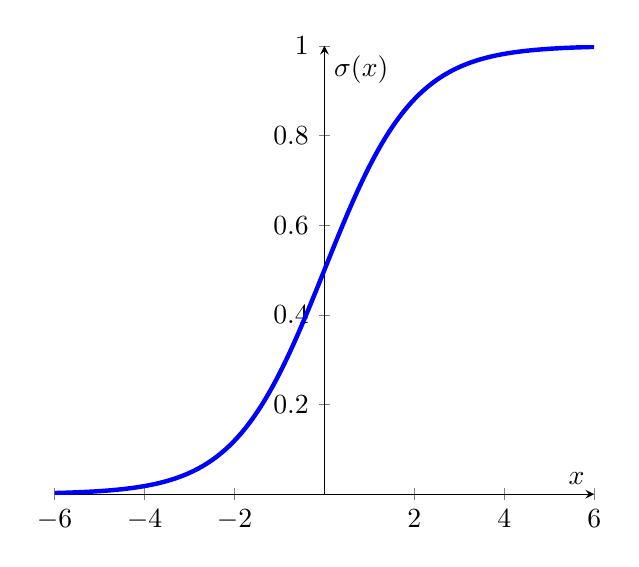
\begin{tikzpicture}
                \begin{axis}[
                    xmax=6, xmin=-6, ymax=1, ymin = 0, samples=200, domain = -6:6,
                    xlabel = {$x$},
                    ylabel = {$\sigma(x)$},
                    xtick={-6,-4,-2, 0, 2,4,6},
                    axis lines = middle
                ]

                \addplot[blue, ultra thick] {1/(1+e^(-x))};
                \end{axis}
            \end{tikzpicture}
        }
        \caption{The sigmoid function}
    \end{figure}

    Assuming that $Y = \{C_1,C_2\}$, we can manipulate Bayes' rule in the following way:
    \[\begin{split}
        \Pr[C_1 \mid x,D] & = \frac{\Pr[x \mid C_1,D] \cdot \Pr[C_1 \mid D]}{\Pr[x \mid D]} \\
        & = \frac{\Pr[x \mid C_1,D] \cdot \Pr[C_1 \mid D]}{\Pr[x \mid C_1,D] \cdot \Pr[C_1 \mid D] + \Pr[x \mid C_2,D] \cdot \Pr[C_2 \mid D] } \\
        & = \frac{1}{1+\dfrac{\Pr[x \mid C_2,D] \cdot \Pr[C_2 \mid D] }{\Pr[x \mid C_1,D] \cdot \Pr[C_1 \mid D]}} \\
     \end{split}\]

    By setting $\alpha = \ln \dfrac{\Pr[x \mid C_1,D] \cdot \Pr[C_1 \mid D] }{\Pr[x \mid C_2,D] \cdot \Pr[C_2 \mid D]}$, we get the sigmoid function $\sigma(\alpha)$.

    Consider now the parametric model where $\Pr[x \mid C_i,D]$ has the normal distribution $\mathcal{N}(x; \mu_i, \Sigma)$, where $\mu_i$ is the mean and $\Sigma$ is a covariance matrix. We have that:
    \[\alpha = \ln \dfrac{\Pr[x \mid C_1,D] \cdot \Pr[C_1 \mid D] }{\Pr[x \mid C_2,D] \cdot \Pr[C_2 \mid D]} = \ln \dfrac{\mathcal{N}(x; \mu_1, \Sigma) \cdot \Pr[C_1 \mid D] }{\mathcal{N}(x; \mu_2, \Sigma) \cdot \Pr[C_2 \mid D]} = w^Tx+w_0\]
    where:
    \[w = \Sigma^{-1} (\mu_1 - \mu_2) \qquad\qquad w_0 = -\frac{1}{2} \mu_1^T \Sigma^{-1} \mu_1 + \frac{1}{2} \mu_2^T \Sigma^{-1} \mu_2 + \frac{\Pr[C_1 \mid D]}{\Pr[C_2 \mid D]}\]

    where $\Pr[C_1 \mid D] = p$ and $\Pr[C_2 \mid D] = 1-p$. To summarize, we have that:
    \[\begin{array}{ccc}
        \Pr[C_1 \mid x,D] = \sigma(w^Tx-w_0) &\qquad\qquad& \Pr[C_2 \mid x,D] = 1- \sigma(w^Tx-w_0) \\\\
        \Pr[x \mid C_1,D] = \mathcal{N}(x; \mu_1, \Sigma) &\qquad\qquad& \Pr[x \mid C_2,D] = \mathcal{N}(x; \mu_2, \Sigma) \\\\
        \Pr[C_1 \mid D] = p &\qquad\qquad& \Pr[C_2 \mid D] = 1-p 
    \end{array}\]
    
    This allows us to easily automatize the computation of such probability since we can skip the computation of the logarithm. However, to achieve this we still have to estimate the values of $\mu_1, \mu_2, p$ and $\Sigma$. Given data set $D = \{(x_n,t_n) \mid i \in [N]\}$, where $t_i = 1$ if $x_i$ is in class $C_1$ and $t_i = 0$ otherwise. Let $N_1$ be the number of samples in $D$ belonging to $C_1$ and $N_2$ be the number of samples in $C_2$ ($N = N_1+N_2$). The maximum-likelihood solution here is given by:
    \[\Pr[t \mid p, \mu_1, \mu_2, \Sigma] = \prod_{i = 1}^N (p \; \mathcal{N}(x_i; \mu_1, \Sigma))^{t_i} ((1-p) \; \mathcal{N}(x_i; \mu_2, \Sigma))^{1-t_i}\]

    After maximizing the logarithmic likelihood, we always obtain that:
    \[\begin{array}{ccc}
        \widehat \mu_1 = \dfrac{1}{N_1} \sum\limits_{i = 1}^N t_i x_i &\qquad\qquad& \widehat \mu_2 = \dfrac{1}{N_2} \sum\limits_{i = 1}^N (1-t_i) x_i \\\\
        \widehat p = \dfrac{N_1}{N} &\qquad\qquad& \widehat \Sigma = \dfrac{N_1}{N} S_1 + \dfrac{N_2}{N} S_2
    \end{array}\]

    where $S_j = \frac{1}{N_j} \sum_{i \in C_j} (x_i - \widehat \mu_j)(x_i - \widehat \mu_j)^T$.

    More generally, when $Y = \{C_1, \ldots, C_k\}$, the dataset is formalized as $D = \{(x_i, t_i) \mid i \in [N]\}$, where $t_i$ is a one-hot indicator vector with $t_{i,j} = 1$ if and only if $x_i$ is in class $C_j$. In this case, the estimate is given by:
    \[\Pr[C_j \mid x] = \frac{\Pr[x \mid C_j,D] \cdot \Pr[C_j,D]}{\sum_{h = 1}^k \Pr[x \mid C_h,D] \cdot \Pr[C_h \mid D]} = \frac{e^{\alpha_j}}{\sum_{h = 1}^k e^{\alpha_h}}\]

    where $\alpha_h = \ln \Pr[x \mid C_h] \Pr[C_h]$. This model is called \textbf{Gaussian Naïve Bayes classification}, where $\forall j \in [k]$ we have: 
    \[\begin{array}{ccc}
        \widehat \Pr[C_j \mid D] = \widehat p_j = \dfrac{N_j}{N} &\qquad\qquad& \Pr[x \mid C_j,D] = \mathcal{N}(x; \mu_j, \Sigma)\\\\
        \widehat \mu_j = \dfrac{1}{N_j} \sum\limits_{i = 1}^N t_{i,j} x_i &\qquad\qquad& \widehat \Sigma = \sum_{j = 1}^k \dfrac{N_j}{N} S_j
    \end{array}\]

    where $S_j = \frac{1}{N_j} \sum_{i \in C_j} (x_i - \widehat \mu_j)(x_i - \widehat \mu_j)^T$. The use of matrix-like computation can be further extended by also modeling other elements as matrices. For instance, given a problem $f : \R^d \to Y$, a dataset $D = \{(x_i, t_i) \mid i \in [N]\}$ can also be represented as $\abk{X,t}$, where $X$ is an $N \times d$ matrix of input values and $t$ is a vector of $N$ output values.

    To make notation more compact, we set $\widetilde{w} = \smat{w_0 \\ w}$ and $\widetilde{x} = \smat{1 \\ x}$ in order to get:
    \[a_h = w^Tx + w_0 = \widetilde{w}^T\widetilde{x}\]

    The maximum-likelihood solution for a parametric model $M_\Theta$ of dataset $D = \abk{X, t}$ with $\Pr[t \mid \Theta, X]$ is thus given by:
    \[\Theta^* \in \argmax_{\Theta} \ln \Pr[t \mid \Theta, X]\]
    
    When $M_\Theta$ belongs to the exponential family, the probability $\Pr[t \mid \theta, X]$ can be expressed in the form $\Pr[t \mid \widetilde{w}, X]$
    \[\Theta^* \in \argmax_{\widetilde{w}} \ln \Pr[t \mid \widetilde{w}, X]\]

    \subsection{Probabilistic discriminative models}

    Consider a classification problem $f : \R^d \to Y$ where $X \subseteq \R^d$ and a dataset $D = \abk{X,t} = \{(x_i,t_i) \mid i \in [N]\}$, with $t_i \in \{0,1\}$.
    Differently from generative models, in \textbf{probabilistic discriminative models}, to estimate $\Pr[C \mid x, D]$ for a new instance $x \in X-X_D$ and a class $C \in Y$, we directly estimate the probability:
    \[\Pr[C_j \mid \widetilde{x}, D] = \frac{e^{\alpha_j}}{\sum_{h = 1}^k e^{\alpha_h}}\]
    without using Bayes' rule, where $\alpha_h = \widetilde{w}^T \widetilde{x}$. In this case, the maximum-likelihood is still given by:
    \[\Theta^* \in \argmax_{\widetilde{w}} \ln \Pr[t \mid \widetilde{w}, X]\]

    The typical example of discriminative model is \textbf{logistic regression}. Suppose that we are working with only two classes. The probability $\Pr[t \mid \widetilde{w},X]$ -- recall that $D = \abk{X,t}$ -- is given by:
    \[\Pr[t \mid \widetilde{w}, X] = \prod_{i = 1}^N p_i^{t_i} (1-p_i)^{1-t_i}\]
    where $p_i = \Pr[C_1 \mid \widetilde{x_i}] = \sigma(\widetilde{w}^T \widetilde{x_i})$. By applying the negative logarithm, we obtain a new type of error function: the \textbf{cross-entropy error function}.

    \begin{frameddefn}{Cross-entropy error function}
        Given a classification problem $f : \R^d \to Y$ and a dataset $D = \abk{X,t}$, the \textbf{cross-entropy} (or \textit{negative log likelihood}) error function is defined as:
        \[E(\widetilde{w}) = - \ln \Pr[t \mid \widetilde{w}, X] = - \sum_{i = 1}^N t_i \ln p_i + (1-t_i) \ln (1-p_i)\]
    \end{frameddefn}

    Logistic regression is based on solving the following optimization problem:
    \[\widetilde{w}^* \in \argmin_{\widetilde{w}} E(\widetilde{w})\]

    There are many efficient ways to solve this problem. The most common one is the \textbf{iteratively reweighted least squares (IRLS)} method, based on \textit{Newton-Raphson iterative method}, which uses derivatives to get closer and closer to the optimal solution. In particular, since we're working with higher dimensions, we'll be using the concept of gradient and gradient descent.
    
    \begin{enumerate}
        \item First, compute the gradient of the error with respect to $\widetilde{w}$:
        \[\nabla E(\widetilde{w}) = \sum_{i = 1}^N (p_i - t_i) \widetilde{x_i}\]

        \item Apply the gradient descent step by setting
        \[\widetilde{w} := \widetilde{w} - H(\widetilde{w})^{-1} \nabla E(\widetilde{w})\]
        where $H(\widetilde{w})$ is the Hessian matrix of $E(\widetilde{w})$, i.e. $H(\widetilde{w}) = \nabla \nabla E(\widetilde{w})$.

        \item Repeat until a certain improvement treshold is reached or after a fixed number of iterations
    \end{enumerate}

    \begin{framedobs}{Gradient}
        For those who aren't confident with multivariate calculus, the gradient of a function $f : \R^n \to \R$ is defined as:
        \[\nabla f(x) = \smat{\frac{\partial  f}{\partial  x_1}(x) \\ \vdots \\ \frac{\partial  f}{\partial  x_n}(x)}\]
        In other words, the gradient of $f$ is the vector whose components are the partial derivatives of $f$ with respect to the components of the input
    \end{framedobs}

    These computation can also be made more compact and immediate -- thus the strength of this model:
    \[\nabla E(\widetilde{w}) = \widetilde{X} ^T (p(\widetilde{w}) - t)\]
    \[H(\widetilde{w}) = \widetilde{X}^T R(\widetilde{w}) \widetilde{X}\]

    where $p(\widetilde{w}) = \smat{p_1 & \cdots & p_N}^T$, $\widetilde{X} = \smat{\widetilde{x_1} & \cdots & \widetilde{x_N}}$ and $R(\widetilde{w})$ is the diagonal matrix where $r_{i,i} = p_i(1-p_i)$.

    \begin{framedalgo}{Iterative reweighted least squares (IRLS)}
        Given a classification problem $f : \R^d \to Y$, where $Y = {C_1, C_2}$, and a dataset $D = \abk{X,t}$, the algorithm solves the optimization problem $\widetilde{w}^* \in \argmin_{\widetilde{w}} E(\widetilde{w})$.

        \begin{algorithmic}
            \Function{IRLS}{$Y,X,t$}
                \State{$\widetilde{w} = 0$}
                \Do
                    \State{$\widetilde{w} = \widetilde{w}-(\widetilde{X}^T R(\widetilde{w}) \widetilde{X})^{-1} \widetilde{X}^T(p(\widetilde{w})- t)$}

                \doWhile{$E(\widetilde{w})$ decreases}
            \EndFunction
        \end{algorithmic}
    \end{framedalgo}

    \chapter{Linear models}

    \section{Linear models for classification}

    In linear models, we're interested in studying classification problems $f : \R^d \to Y$ with a dataset whose instances are \textbf{linearly separable}. A dataset is said to be linearly separable when there exists a hyperplane that separates the instance space into two regions such that differently classified instances lie on different regions.

    \begin{figure}[H]
        \centering
            \begin{tabular}{ccc}
                \begin{tikzpicture}[scale=0.8]
                    \begin{axis}[%
                        xmax=6, xmin=0, ymax=8, ymin = 0, domain = 0:6,
                        axis lines = middle,
                        scatter/classes={%
                            a={mark=+, draw=red},%
                            b={mark=-, draw=blue}}
                    ]

                    \addplot[scatter,only marks,%
                        scatter src=explicit symbolic]%
                        table[meta=label] {
                            x y label
                            1 7 a
                            1.3 6.8 a
                            1.2 7.1 a
                            1.3 7.2 a
                            1.5 6.5 a
                            1.7 7.8 a
                            1.1 7.4 a
                            1.8 7.5 a

                            5 1 b
                            4.7 1.3 b
                            4.9 1.5 b
                            4.2 0.7 b
                            4.6 1.7 b
                            5.8 1.6 b
                        };
                    \addplot[black, ultra thick] {(3/2)*x};
                    \end{axis}
                \end{tikzpicture}

                &\qquad\qquad&

                \begin{tikzpicture}[scale=0.8]
                    \begin{axis}[%
                        xmax=6, xmin=0, ymax=8, ymin = 0, domain = 0:6,
                        axis lines = middle,
                        scatter/classes={%
                            a={mark=+, draw=red},%
                            b={mark=-, draw=blue}}
                    ]

                    \addplot[scatter,only marks,%
                        scatter src=explicit symbolic]%
                        table[meta=label] {
                            x y label
                            1 7 a
                            1.2 7.1 a
                            0.9 7.2 a
                            5 1 a
                            5.2 0.7 a
                            5.1 1.2 a

                            1 1 b
                            1.1 0.9 b
                            1.2 1.1 b
                            5 7 b
                            4.9 6.8 b
                            5.2 7.1 b
                        };
                    \end{axis}
                \end{tikzpicture}
            \end{tabular}
        \caption{A linearly separable dataset (left) and a non-linearly separable one (right)}
    \end{figure}

    The functions describing such hyperplanes are called \textbf{linear discriminant functions}. Suppose that $Y = \{C_1, \ldots, C_k\}$. We define $k$ linear functions:
    \[y_1(x) = w_1^Tx + w_{1_0} = \widetilde{w_1}^T \widetilde{x} \qquad \cdots \qquad y_k(x) = w_k^T x + w_{k_0} = \widetilde{w_k}^T \widetilde{x}\]
    
    where $\widetilde{w_h} = \smat{w_{h_0} \\ w_h}$ and $\widetilde{x} = \smat{1 \\ x}$. Each instance $x \in \R^d$ gets classified as $C_j$ if the $y_j(x)$ is the one with maximum value.
    \[C_j \in \argmax_{C_h \in Y} y_h(x)\]

    In particular, we observe that for each $C_j, C_{j'}$ the hyperplane $(\widetilde{w_j} - \widetilde{w_{j'}})^T \widetilde{x} = 0$ acts as a \textbf{decision boundary}, splitting the regions of points classified as either $C_j$ or $C_{j'}$. 

    \begin{figure}[H]
        \centering
        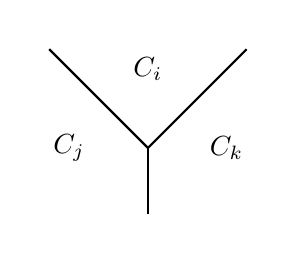
\begin{tikzpicture}[-,>=stealth,shorten >=1pt,auto,node distance=1cm, thick,main node/.style={scale=0.9,circle,draw,font=\sffamily\normalsize}]

            \node[] (1) []{};
            \node[] (2) [above left of = 1, xshift=-20, yshift=20]{};
            \node[] (3) [above right of = 1, xshift=20, yshift=20]{};
            \node[] (4) [below of = 1]{};
            \node[] (5) [above of = 1]{$C_i$};
            \node[] (6) [left of = 1]{$C_j$};
            \node[] (7) [right of = 1]{$C_k$};

            \path[every node/.style={font=\sffamily\small}]
                (1.center) edge (2)
                (1.center) edge (3)
                (1.center) edge (4)
            ;
        \end{tikzpicture}

        \caption{Example of how regions get partitioned by a $K$-class discriminant}
    \end{figure}

    Given the following matrix:
    \[y(x) = \smat{y_1(x) \\ \vdots \\ y_k(x)} = \smat{\widetilde{w_1}^T \\ \vdots \\ \widetilde{w_k}^T} \widetilde{x} = \widetilde{W}^T \widetilde{x}\]

    where $\widetilde{W} = \smat{\widetilde{w_1} & \cdots & \widetilde{w_k}}$, learning a linear model is equivalent to estimating the matrix $\widetilde{W}$ for which $y(x) = \widetilde{W}^T \widetilde{X}$ defines the $K$-class discriminant.

    In particular, we'll restrict our interest to models working directly on the samples $x$. All the results that we will discuss also hold if we consider a non-linear transformation of the inputs $\phi(x)$, called \textbf{basis functions}. The idea is to use these transformations to convert the feature space into a linearly separable one in order to apply the discussed methods. In particular, decision boundaries will be linear in the feature space $\phi(x)$ and non-linear in the original space $x$. Clearly, classes that are linearly separable in the feature space $\phi(x)$ may not be as easily separable in the input space $x$.

    \begin{figure}[H]
        \centering
        \includegraphics[scale=0.75]{images/basis_func.png}
        \caption{Example of a basis function being applied on a non-linearly separable feature space, making the property hold on the basis feature space.}
    \end{figure}


    \subsection{Least squares method}

    The first method that we'll discuss is the \textbf{least squares method}. Consider problem $f : \R^d \to Y$ a dataset $D = \{(x_i, t_i) \mid i \in [N]\}$, where each $t$ is a 1-of-$K$ encoding, meaning that $t_{i,j} = 1$ if $x_i \in C_j$, otherwise $t_{i,j} = 0$. We want to find the linear discriminant $y(x) = \widetilde{W}^Tx\widetilde{x}$. Let $\widetilde{X} = \smat{\widetilde{x_1} & \cdots & \widetilde{x_N}}^T$ and let $T = \smat{t_1 & \cdots & t_N}$. We notice that each row of the product $\widetilde{X} \widetilde{W}$ contains the predicted class for the associated input, while the matrix $T$ contains the real class for the input. When the two matrices are equal, the model is perfect. Hence, we want to minimize the difference between such matrices. To do so, we minimize the \textbf{sum-of-squares error function}.

    \begin{frameddefn}{Sum-of-squares error function}
        Given a linearly separable classification problem $f : \R^d \to Y$ and a dataset $D =  \{(x_i, t_i) \mid i \in [N]\}$, the \textbf{sum-of-squares error function} is defined as:
        \[E(\widetilde{W}) = \frac{1}{2} \tr \rbk{(\widetilde{X}\widetilde{W} - T)^T(\widetilde{X}\widetilde{W} - T)}\]
    \end{frameddefn}

    We notice that each entry $a_{i,i}$ on the diagonal of the inner matrix in the above definition is the double of the square of the difference between $x_i$'s predicted class and $t_i$. Hence, the trace of the is equal to the sum-of-squares. The halving factor is just a convention.  

    This minimization problem can be actually solved in a closed form. In fact, we have that:
    \[\widetilde{W} = (\widetilde{X}^T \widetilde{X})^{-1} \widetilde{X}^T T\]

    concluding that:
    \[y(X) = \widetilde{W}^T \widetilde{X} = T^T (\widetilde{X}^{\dagger})^T X\]

    where $\widetilde{X}^{\dagger} = (\widetilde{X}^T \widetilde{X})^{-1} \widetilde{X}^T$ is the \textbf{pseudo-inverse} of $\widetilde{X}$. We observe that this is the first method we have seen where we can actually compute a perfect optimal solution, making this method very easy to use. However, this model still has some problems: the $K$-class discriminant obtained is not robust to \textbf{outliers}, i.e. samples that are very far away from the other samples that are classified with the same class.

    \begin{figure}[H]
        \centering
        \includegraphics[scale=0.6]{images/outliers.png}
        \caption{Example of how outliers \curlyquotes{rotate} the solution}
    \end{figure}

    \subsection{Perceptron}

    Consider a linear classification problem $f : \R^d \to \{-1, +1\}$. A \textbf{perceptron} is a binary classifier that assigns one of two classes to a real-valued input vector. Let $w = \smat{w_0 & w_1 & \cdots & w_d}^T$ be a weight vector and let $x \in \R^{d+1}$ where $x_0 = 1$ -- from now on we'll drop the $\widetilde{w}, \widetilde{x}$ notation. A perceptron is a function $o(x)$ that can be defined in two ways: \textbf{tresholded} or \textbf{untresholded}. In the untresholded case, we have that $o(x) =  w^T{x}$, while in the tresholded case we have that $o(x) = \mathrm{sign}( w^T{x})$, where:
    The perceptron $o(x)$ given by $ w$ is defined as:
    \[\mathrm{sign}( w^T{x}) = \soe{ll}{
        +1 & \text{if } w_0 + w_1x_1 + \ldots + w_dx_d > 0 \\
        -1 & \text{otherwise}
    }\]

    \begin{figure}[H]
        \centering
        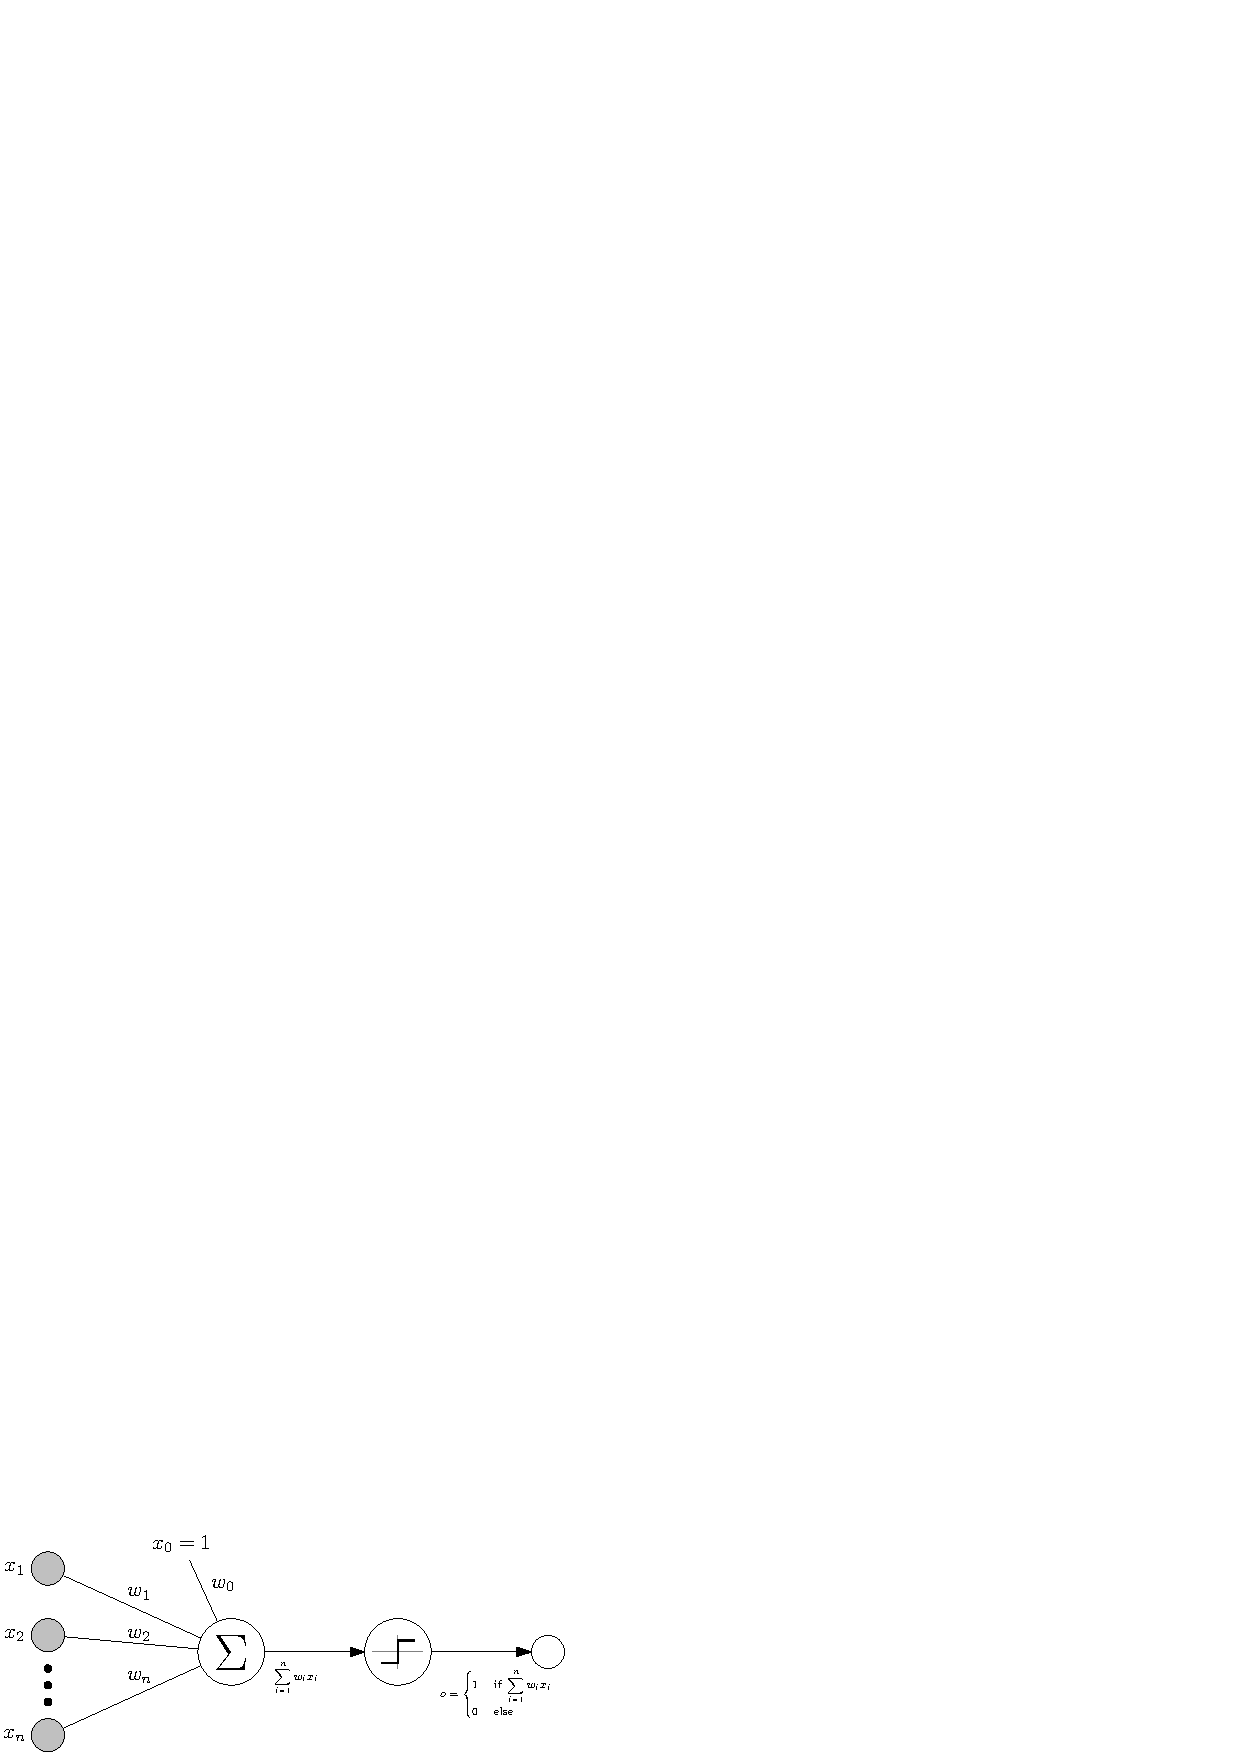
\includegraphics[scale=0.55]{images/perceptron.png}
        \caption{A tresholded perceptron}
    \end{figure}
    
    In both cases, to learn $w$ from a dataset $D = \{(x_i, t_i) \mid i \in [N]\}$, we want to minimize the squared error (\textit{loss function}):
    \[E(w) = \frac{1}{2} \sum_{i = 1}^N (t_i - o(x_i))^2 \]

    Since we're working with real values, the minimization problem can be solved through derivatives and an iterative approach. This is called the \textbf{perceptron training rule}.
    \begin{enumerate}
        \item First, compute the derivative of $E( w)$ with respect to each component of $w_j$ of $ w$
        \[\frac{\partial  E}{\partial  w_j} = \sum_{i = 1}^N (t_i - o(x_i))(-x_{j,i})\]
    
        \item Update each component $w_j$ by setting $ w_j := w_j + \Delta w_j$, where:
        \[\Delta w_j = - \eta \frac{\partial  E}{\partial  w_j} = \eta \sum_{i = 1}^N (t_i - o(x_i))x_{j,i}\]
        with $\eta$ being a small constant called \textit{learning rate}

        \item Repeat until a certain improvement treshold is reached (or after a fixed number of iterations)
    \end{enumerate}
    
    The choice of $\eta$ is \underline{critical}: if $\eta$ is small then each iteration will only slightly move the previous linear discriminant, while if $\eta$ is large each iteration may significantly move the discriminant.
    

    Moreover, when $\eta$ is small, the final solution will either be very close to the samples of the first class or very close to the samples of the second class. In other words, the solution \underline{cannot lie in the middle} of the two sample groups. It can be proven that this procedure will converge if the training data is linearly separable and $\eta$ is sufficiently small. However, convergence doesn't imply termination, hence the terminating condition.

    After learning the optimal $ w$, the predicted class of a new instance $x \in \R^d-\R^d_D$ is -- in both treshholded and untresholded perceptrons -- given by $\mathrm{sign}({w}^T{x})$.
    

    \begin{figure}[H]
        \centering
        \includegraphics[scale=0.9]{images/perceptron_2.png}
        \caption{Two iterations of the perceptron training rule with a small $\eta$ value. The vector $w$ is represented by the black arrow, while the vector $\delta w$ is represented by the red arrow. The green-circled samples circled are misclassified, hence their feature vector is considered for the next iteration.}
    \end{figure}

    \newpage

    \subsection{Fisher's linear discriminant}

    Consider a linear classification problem $f : \R^d \to \{C_1, C_2\}$. We want to determine a linear discriminant $y = {w}^T {x}$ with a vector ${w} = \smat{w_0 & w_1 & \cdots w_d}^T$ for which $x \in C_1$ if $y \geq -w_0$ and $x \in C_2$ otherwise.

    Consider a dataset with $N_1$ points in $C_1$ and $N_2$ points in $C_2$. Let $m_1$ and $m_2$ be the average of their distributions:
    \[m_1 = \frac{1}{N_1} \sum_{x_i \in C_1} x_i \qquad\qquad m_2 = \frac{1}{N_2} \sum_{x_i \in C_2} x_i\]

    To maximize class separation, we have to adjust the value of ${w}$ in order to maximize the function $J( w) = {w}^T (m_2 - m_1)$, subject to $\norm{{w}} = 1$ -- implying that ${w} \propto m_2 - m_1$.
    
    Consider the segment connecting the points represented by $m_1$ and $m_2$. Then, the bisector of this segment will always define the maximal linear discriminant ${w}$. In fact, if we consider the projections of all the points in the dataset on a line parallel to the segment we get an almost correct separation of the two classes. However, in case of oriented covariance, some samples may get misclassified.

    \begin{figure}[H]
        \centering
        \includegraphics[scale=0.65]{images/fisher_1.png}
        \caption{The blue and red crosses represent the average points of the two distributions. The green bisector of green segment connecting the two crosses is the almost valid linear discriminant. The colored bars represent the number of samples projected on the dashed line perpendicular to the green segment.}
        \label{fisher_1}
    \end{figure}

    From \Cref{fisher_1}, it's easy to see that in order to get a perfect linear discriminant it would suffice to slightly rotate this bisector. To achieve this, \textbf{Fisher's discriminant} allows some degree of freedom. In particular, the \textit{Fisher criterion} is defined as the function:
    \[J( w) = \frac{{w}^T S_B {w}}{{w}^T S_W {w}}\]

    where $S_B$, called the \textit{between class scatter}, is defined as:
    \[S_B = (m_2-m_1)(m_2-m_1)^T\]
    and where $S_W$, called the \textit{within class scatter}, is defined as:
    \[S_W = \sum_{x_i \in C_1} (x_i - m_1)(x_i - m_1)^T + \sum_{x_i \in C_2} (x_i - m_2)(x_i - m_2)^T\]

    Again, we want to maximize $J( w)$. Using derivatives -- hence by solving the equation $\frac{d J}{d  w} = 0$ -- we get that the optimal solution ${w}^*$ is proportional to $S_W^{-1}(m_2 - m_1)$. In particular, an almost optimal solution can be achieved by directly setting ${w} = S_W^{-1}(m_2 - m_1)$ -- the optimal solution is proportional to this one -- where $w_0 = {w}^Tm$ with $m$ being the global average of all samples.

    \begin{figure}[H]
        \centering
        \includegraphics[scale=0.8]{images/fisher_2.png}
        \caption{The optimal solution depends on the inverse of the within class scatter.}
    \end{figure}

    For a multiple classes generalization, we consider the discriminant $y = {W}^Tx$, where we want to maximize:
    \[J({W}) = \tr\rbk{({W} S_W {W}^T)({W} S_W {W}^T)^{-1}}\]

    In perceptrons, we saw how the final discriminant is always very close to one of the two datasets. Using Fisher's discriminant, instead, the final discriminant is nothing more than a rotation of a bisector, hence it will always lie exactly in the middle of the two sample groups. But which of the two solutions is better? For samples that are in the dataset, the two solutions are equivalent: all the samples will be correctly classified. For new samples, instead, we expect Fisher's solution to have a lower probability of misclassification.

    \begin{figure}[H]
        \centering
        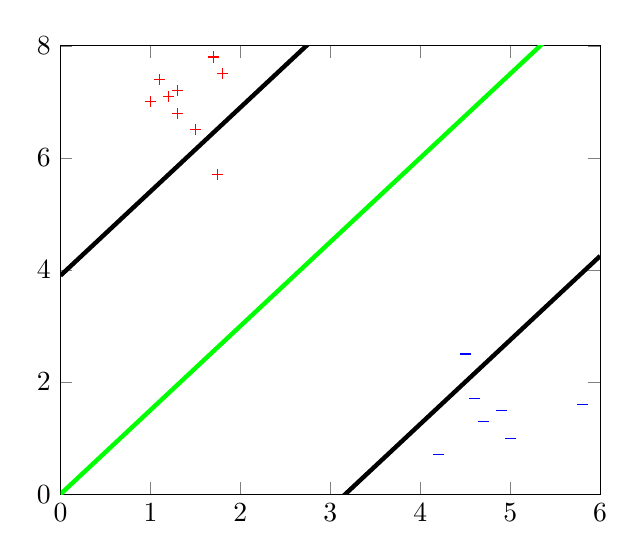
\begin{tikzpicture}
            \begin{axis}[%
                xmax=6, xmin=0, ymax=8, ymin = 0, domain = 0:6,
                scatter/classes={%
                    a={mark=+, draw=red},%
                    b={mark=-, draw=blue}}
            ]

            \addplot[scatter,only marks,%
                scatter src=explicit symbolic]%
                table[meta=label] {
                    x y label
                    1 7 a
                    1.3 6.8 a
                    1.2 7.1 a
                    1.3 7.2 a
                    1.5 6.5 a
                    1.7 7.8 a
                    1.1 7.4 a
                    1.8 7.5 a

                    5 1 b
                    4.7 1.3 b
                    4.9 1.5 b
                    4.2 0.7 b
                    4.6 1.7 b
                    5.8 1.6 b

                    1.75 5.7 a
                    4.5 2.5 b

                };
            \addplot[green, ultra thick] {(3/2)*x};
            \addplot[black, ultra thick] {(3/2)*x + 3.9};
            \addplot[black, ultra thick] {(3/2)*x - 4.75};
            \end{axis}
        \end{tikzpicture}
        \caption{The green discriminant may be found through Fisher's criterion. The two black lines may be found through perceptrons. Fisher's discriminant makes no errors, while both perceptron discriminants make an error.}
    \end{figure}


    \subsection{Support Vector Machines}

    After discussing how Fisher's discriminant is (on average) better than perceptrons due to how the generated discriminant has a good margin of error from both sample groups, hence lower probability of misclassifying samples, we can build a new model based on this idea. \textbf{Support Vector Machines (SVM)} aims at maximizing such margin, providing better accuracy.

    \begin{figure}[H]
        \centering
        \includegraphics[scale=0.25]{images/svm.png}
        \caption{General idea behind SVMs}
    \end{figure}

    Consider a binary classification problem $f : \R^d \to \{+1, -1\}$ and a linearly separable dataset $D = \{(x_i,t_i) \mid i \in [N]\}$ where $t_i \in \{+1, -1\}$. Then, there is a function $y(x) = w^Tx + w_0$ such that forall $i \in [N]$ it holds that $y(x_i) > 0$ if $t_i = +1$ and $y(x_i) < 0$ if $t_i = -1$, implying that:
    \[\forall i \in [N] \;\; t_i y(x_i) > 0\]

    Let $x_k$ be the point of $D$ closest to the affine hyperplane $h :  w^Tx + w_0 = 0$. Then, the margin is the smallest distance from $x_k$ and $h$, which is equal to $\frac{\abs{y(x_k)}}{\norm{w}}$. Using the fact that $\abs{y(x_i)} = t_i y(x_i)$, we can compute the margin by minimizing such distance:
    \[\min_{i \in [N]} \frac{\abs{y(x_i)}}{\norm{w}} = \frac{1}{\norm{w}} \min_{i \in [N]} t_i(w^Tx + w_0)\]

    Thus, to find the hyperplane which maximizes such margin, we can solve the following optimization problem:
    \[w^*, w_0^* \in \argmax_{w, w_0} \frac{1}{\norm{w}} \min_{i \in [N]} t_i(w^Tx + w_0)\]
    
    After the maximum margin hyperplane $h^* : w^{*^T}x+w_0^*$ is found, there will be at least two closest points $x_k^{\oplus}$ and $x_k^{\ominus}$, one for each class.

    We also notice that, since this doesn't affect the solution, we can also rescale all the points in such a way that $t_i(w^Tx + w_0) = 1$ holds for all $i \in [N]$. Hence, we consider the canonical representation where $t_i(w^Tx + w_0) \geq 1$ for all $i \in [N]$. In this setup, the optimal solution is given by:
    \[w^*, w_0^* \in \argmax_{w, w_0} \frac{1}{\norm{w}} \min_{i \in [N]} t_i(w^Tx + w_0) = \argmax_{w, w_0} \frac{1}{\norm{w}} = \argmin_{w, w_0} \frac{1}{2} \norm{w}^2\]
    subject to $t_i(w^Tx + w_0) \geq 1$ for all $i \in [N]$. Hence, we get a quadratic programming optimization problem, which can be solved through the Lagrangian method. For our interest, we won't dive into how this problem is solved, considering directly its solution:
    \[w^* = \sum_{i = 1}^{N} a_i^* t_i x_i\]

    where each $a_i^*$ is a Lagrangian multiplier, a byproduct of the following Lagrangian optimization problem:
    \[{L}(a) = \sum_{i = 1}^N a_i - \frac{1}{2} \sum_{i = 1}^N \sum_{j = 1}^N a_i a_j t_i t_j x_i^T x_j\]
    subject to:
    \[a_i \geq 0\qquad \forall i \in [N]\]
    \[\sum_{i = 1}^N a_i t_i = 0\qquad \forall i \in [N]\]

    \begin{framedprop}{Karush-Kuhn-Tucker (KKT) condition}
        Given the above solution to the maximal margin hyperplane problem:
        \[w^* = \sum_{i = 1}^{N} a_i^* t_i x_i\]
        For each $i \in [N]$, it holds that either $a_i^* = 0$ or $t_i y(x_i) = 1$
    \end{framedprop}

    The KKT conditions ensures that, in the canonical representation, every time $t_i y(x_i) \neq 1$ then $a_i^* = 0$, meaning that these terms do not contribute to the solution. Hence, the \textbf{support vectors} are given by each $x_i$ such that $t_i y(x_i) = 1$ (and thus $a_i^* > 0$).
    \[SV = \{x_i \mid i \in [N], t_i y(x_i) = 1\}\]

    Hence, we get that:
    \[y(x) = \sum_{x_i \in SV} a_i^* t_i x^T x_i + w_0^*\]
    
    To compute $w_0^*$, we pick a support vector $x_k \in SV$. Since $x_k$ satisfies $t_ky(x_k) = 1$, we get that:
    \[t_k \rbk{\sum_{x_i \in SV} a_i^* t_i x_k^T x_i + w_0^*} = 1\]

    Moreover, since $t_i \in \{-1,+1\}$, we know that $t_i^2 = 1$, concluding that:
    \[w_0^* = t_k - \sum_{x_i \in SV} a_i^* t_i x_k^T x_i\]

    The optimization problem for determining $w^*,w_0^*$ ($d + 1$ dimensions) is thus transformed into an optimization problem for determining $a^*$ ($\abs{D}$ dimensions). This method is very efficient when $d \ll \abs{D}$, in particular when $d$ is large or infinite.

    A more stable solution can be obtained by averaging over all support vectors:
    \[w_0^* = \frac{1}{\abs{SV}} \sum_{x_k \in SV} \rbk{t_k - \sum_{x_i \in SV} a_i^* t_i x_k^T x_i}\]
    
    In conclusion, the maximum margin hyperplane $h^* : y(x) = 0$ is given by:
    \[y(x) = \sum_{x_i \in SV} a_i^* t_i x^T x_i + \frac{1}{\abs{SV}} \sum_{x_k \in SV} \rbk{t_k - \sum_{x_i \in SV} a_i^* t_i x_k^T x_i}\]

    The classification of new instance $x \in \R^d-\R^d_D$ is determined by $\mathrm{sign}(y(x))$. 

    We observe that this method can also be applied when the dataset is \textit{almost} linearly separable, i.e. when only a few points are on the wrong side, with addition of some \textit{slack variables} $\xi_i$ for all $i \in [N]$:
    \begin{itemize}
        \item We set $\xi_i = 0$ if the point $x_i$ is on the correct side of the decision boundary and outside the margin (or on its border)
        \item We set $0 < \xi_i \leq 1$ if the point $x_i$ is in the correct side of the decision boundary but inside the margin
        \item We set $\xi_i \geq 1$ if the point $x_i$ is in the wrong side of the decision boundary
    \end{itemize}

    These slack variables are used to a \textit{soft margin constraint} version of the optimization problem :
    \[w^*, w_0^* \in \argmin_{w, w_0} \frac{1}{2} \norm{w}^2 + C \sum_{i = 1}^N \xi_i\]
    
    subject to:
    \[t_i y(x_i) \geq 1 - \xi_i\qquad \forall i \in [N]\]
    \[\xi_i \geq 0\qquad \forall i \in [N]\] 
    where $C$ is a constant (usually the inverse of a regularization coefficient).

    \begin{figure}[H]
        \centering
        \includegraphics[scale=0.8]{images/svm_2.png}
        \caption{Example of slack variable settings.}
    \end{figure}

    \newpage

    \section{Linear models for regression}

    We recall that regression problems consist in functions where the co-domain is real valued. In particular, in this section we'll consider functions of the form $f : \R^d \to \R$. Here, the dataset $D = \{(x_i, t_i) \mid i \in [N]\}$ associated real value $t_i$ to the input point $x_i$. 

    We recall that regression typically involves the approximation of some function. In particular, \textbf{linear regression} involves linear models capable of approximating linear functions. As in the previous section, we consider functions of the form $y( x; {w}) = {w}^T{x}$, where ${x} = \smat{1 & x_1 & \cdots & x_d}$ is the input and ${w} = \smat{w_0 & w_1 & \cdots & w_d}^T$ are the parameters of the model.

    \begin{figure}[H]
        \centering
        \includegraphics[scale=0.7]{images/lin_reg_2.png}
        \caption{Example of approximation through linear regression.}
    \end{figure}

    As for linear classification, in linear regression we can also consider linear basis function models, where we apply a non-linear function $\phi$ on the input variables $y({x};  w) = {w}^T \phi({x})$, where we assume $\phi(x_0) = 1$. By definition, these models are still linear in ${w}$.

    One of the most commonly used basis function in linear regression is the polynomial function up to some degree. For instance, assuming that $d = 1$, a common basis function $\phi : \R \to \R^M$ is $\phi({x}) = \smat{1 & x & x^2 & \cdots & x^M}^T$ in order to get:
    \[y = w_0 + w_1x + w_2x^2 + \ldots + w_M x^M\]

    Here, the choice of the degree $M$ is \underline{critical}: a small degree will underfit the function, while a large degree will overfit it. Other common choices include the radial function, the sigmoid function and the hyperbolic tangent function.
    
    \begin{figure}[H]
        \centering
        \includegraphics[scale=0.8]{images/lin_reg_3.png}
        \caption{The green line is the true function. $M = 0$ and $M=1$ underfit the function, while $M = 9$ overfits it}
    \end{figure}

    Common algorithms for linear regression include:
    \begin{itemize}
        \item Maximum likelihood and least squares
        \item Sequential Learning
    \end{itemize}

    In the \textbf{maximum likelihood and least squares} method, a target value $t$ is given by $y( x;  w)$, affected by some additive noise $\varepsilon$, i.e. $t = y( x;  w) + \varepsilon$. For instance, assuming \textit{Gaussian noise}, we have that the probability of having an error of magnitude $\varepsilon$ with precision $\beta$ is given by:
    \[\Pr[\varepsilon \mid \beta] = \mathcal{N}(\varepsilon \mid 0, \beta^{-1})\]

    Hence, we get that:
    \[\Pr[t \mid {x}, {w}, \beta] = \mathcal{N}(t \mid y({x}; {w}), \beta^{-1})\]

    Moreover, assuming that the observations $t_1, \ldots, t_N$ are i.i.d., the maximum likelihood function is given by:
    \[\Pr[t_1, \ldots, t_N \mid {x_1}, \ldots {x_N}, {w}, \beta] = \prod_{i = 1}^N \mathcal{N}(t_i \mid {w}^T \phi({x_i}), \beta^{-1})\]

    By applying the logarithmic, we get that:
    \[\begin{split}
        \ln \Pr[t_1, \ldots, t_N \mid {x_1}, \ldots {x_N}, {w}, \beta] &= \sum_{i = 1}^N \ln \mathcal{N}(t_i \mid {w}^T \phi({x_i}), \beta^{-1}) \\
        &= -\beta \underbrace{\frac{1}{2} \sum_{i = 1}^N (t_i - {w}^T \phi({x_i}))^2}_{E_D({w})} - \frac{N}{2} \ln (2 p \beta^{-1})
     \end{split}\]

    We notice that the sum-of-square error $E_D({w}) = \frac{1}{2} \sum_{i = 1}^N (t_i - {w}^T \phi({x_i}))^2$ lies inside the previous calculation, hence the name of this method.

    Thus, we conclude that the maximum likelihood (under zero-mean Gaussian noise assumption) corresponds to the least square error minimization:
    \[\argmax_{{w}} \Pr[t_1, \ldots, t_N \mid {x_1}, \ldots {x_N}, {w}, \beta] = \argmin_{{w}}  \frac{1}{2} \sum_{i = 1}^N (t_i - {w}^T \phi({x_i}))^2\]

    We also notice that we can express $E_D({w})$ as:
    \[E_D({w}) = \frac{1}{2}({t} - \Phi {w})^T({t} - \Phi {w})\]

    where:
    \[{t} = \smat{t_1 \\ \vdots \\ t_N} \qquad\qquad \Phi = \smat{\phi(x_1)_0 & \phi(x_1)_1 & \cdots & \phi(x_1)_M \\
    \phi(x_2)_0 & \phi(x_1)_1 & \cdots & \phi(x_1)_M \\
    \vdots & \vdots & \ddots & \vdots \\
    \phi(x_N)_0 & \phi(x_N)_1 & \cdots & \phi(x_N)_M \\}\]
    
    The optimality condition is reached when $\nabla E_D({w}) = 0$, which happens if and only if $\Phi^T \Phi {w} = \Phi^T {t}$, concluding that:
    \[{w}_{ML} = (\Phi^T \Phi)^{-1} \Phi^T t = \Phi^{\dagger} t \]

    In the \textbf{sequential learning} method, we use a \textit{stochastic gradient descent}, where in each iteration we set:
    \[\widehat{{w}} := \widehat{{w}} - \eta \nabla E_{\{x_i\}}(w) = \widehat{{w}} + \eta (t_i - \widehat{{w}}^T \phi(x_i)) \phi(x_i)\]
    where $i \in [N]$ is randomly chosen, $\eta$ is a small parameter called \textit{learning rate} and $E_{\{x_i\}}$ is the error on the $i$-th sample.

    To control overfitting, we use a technique called \textbf{regularization}, where we consider:
    \[\argmin_{{w}} E_D({w}) + \lambda E_W({w})\]
    with $\lambda > 0$ being the \textit{regularization factor}. For the vector $E_W({w})$, we commonly chose the value:
    \[E_W({w}) = \frac{1}{2}{w}^T {w}\]

    While other choices include:
    \[E_W({w}) = \sum_{j = 0}^M \abs{w_j}^q\]
    for some $q > 0$.

    \begin{figure}[H]
        \centering
        \includegraphics[scale=0.71]{images/lin_reg_4.png}

        \includegraphics[scale=0.9]{images/lin_reg_5.png}

        \includegraphics[scale=0.9]{images/lin_reg_6.png}
        \caption{Examples of linear regression without regularization (top), with regularization factor $\ln \lambda = -18$ (middle) and with regularization factor $\ln \lambda = 0$ (bottom)}
    \end{figure}

    \newpage

    \chapter{Advanced techniques}

    \section{Kernel methods}

    So far, we have considered input objects that are represented by a vector $x \in \R^d$ or by a non-linear transformation $\phi(x)$ that makes the dataset linearly separable. But what about objects of different length or infinite dimensions (e.g. strings, trees, images, ...)? To work with these type of objects, we need to use \textbf{kernel functions}, i.e. functions that evaluate the similarity between two objects, mapping them to a set of points on the Euclidean space.

    \begin{frameddefn}{Kernel function}
        Given two multi-dimensional inputs $x, x' \in \mathcal{X}$ of potentially different dimensions, a \textbf{kernel function} is a function $K : \mathcal{X} \times \mathcal{X} \to \R$ which evaluates the similarity between $x$ and $x'$. 
    \end{frameddefn}

    Usually, kernel functions are also symmetric, i.e. $k(x, x') = k(x', x)$, and non-negative, i.e. $k(x, x') \geq 0$, even though these properties are not strictly required. There are many types of kernel functions, including:
    \begin{itemize}
        \item \textit{Linear}:
        \[k(x,x') = x^Tx'\]
        \item \textit{Polynomial}:
        \[k(x,x') = (\beta x^T x' + \gamma)^d\]
        where $\beta, \gamma \in \R$ and $d \in \N_{> 1}$
        \item \textit{Radial Basis function (RBF)}:
        \[k(x,x') = \exp(-\beta \abs{x-x'}^2)\]
        where $\beta \in \R$
        \item \textit{Sigmoid}:
        \[k(x,x') = \tanh(\beta x^T x' + \gamma)\]
        where $\beta, \gamma \in \R$
    \end{itemize}
    
    The input data in the dataset $D$ must usually be normalized in order for the kernel to be a good similarity measure.
    Several types of normalizations include:
    \begin{itemize}
        \item \textit{Min-max}:
        \[\overline{x} = \frac{x-x_{min}}{x_{max}- x_{min}}\]
        where $x_{max}, x_{min}$ are respectively the maximum and minimum value in $D$
        \item \textit{Standardization}:
        \[\overline{x} = \frac{x-\mu}{\sigma}\]
        where $\mu, \sigma$ are respectively the mean and standard deviation of $D$
        \item \textit{Unit vector}:
        \[\overline{x} = \frac{x}{\norm{x}}\]
    \end{itemize}

    For the rest of this section, we'll be assuming to be working with normalized data.

    \begin{framedprop}{Kernel trick (or kernel substitution)}
        Given a kernel function $k$, whenever an input vector $x$ is used in an algorithm only in the form of an inner product $x^Tx'$ for some $x'$, we replace such inner product with $k(x,x')$
    \end{framedprop}

    When applicable, the kernel trick is valid for any input pair $x,x'$, even those with infinite dimension. Moreover, in presence of a basis function $\phi$ being applied on the feature space, the kernel trick also works: we substitute $\phi(x)^T \phi(x')$ with $k(x,x')$. This also implies that we don't need to know the value of $\phi(x), \phi(x')$, making it very powerful.

    For instance, consider a linear model $y({x}; {w}) = {w}^T {x}$ with dataset $D = \{(x_i, t_i) \mid i \in [N]\}$. Consider the sum-of-squares error function with an additional regularization, defined in the same way as the previous section but without the non-linear transformation applied:
    \[E({w}) = \frac{1}{2} \sum_{i = 1}^N (t_i - {w}^T x_i)^2 + \lambda {w}^T {w}\]

    This error function can be re-written as:
    \[E({w}) = \frac{1}{2}  ({t}-X {w})^T({t}-X {w}) + \lambda \norm{w}^2\]
    
    where ${t} = \smat{t_1 & \cdots & t_N}^T$ is the output vector and $X = \smat{x_1 & \cdots & x_N}^T$ is the design matrix. Here, the optimal solution is obtained by $\nabla E({w}) = 0$, which happens when:
    \[{w^*} = -\frac{1}{\lambda} \sum_{i = 1}^N (t_i - {w}^T {x_i}) {x_i} = \sum_{i = 1}^N \alpha_i x_i\]

    where $\alpha_i = -\frac{1}{\lambda}(t_i - {w}^T {x_i})$. We get that:
    \[y({x}, {w^*}) = \sum_{i = 1}^N \alpha_i x_i^T x\]

    Moreover, we also notice that the optimal solution can also be computed in a matrix-like form. In particular, we have that:
    \[{w^*} = (X^TX + \lambda I_N)^{-1} X^T  t = X^T (XX^T + \lambda I_N)^{-1}  t = X^T \alpha\]

    where $\alpha = (XX^T + \lambda I_N)^{-1} {t}$. As before, we get that:
    \[y({x}, {w^*}) = \sum_{i = 1}^N \alpha_i x_i^T x\]

    The matrix $K = XX^T$ is usually called \textbf{Gram's matrix}.
    \[K = \smat{x_1^T x_1 & \cdots & x_1^T x_N \\
    \vdots & \ddots & \vdots \\
    x_N^T x_1 & \cdots & x_N^T x_N }\]

    By applying any kernel trick with a kernel $k$, we get that:
    \[y({x}, {w^*}) = \sum_{i = 1}^N \alpha_i k(x_i, x)\]

    while Gram's matrix becomes:
    \[K = \smat{k(x_1,x_1) & \cdots & k(x_1, x_N) \\
    \vdots & \ddots & \vdots \\
    k(x_1,x_n) & \cdots & k(x_N,x_N)}\]

    The kernel trick comes in handy mostly in Support Vector Machines (SVM). We saw how in this model the optimal solution has the form:
    \[{w^*} = \sum_{i = 1}^N \alpha_i x_i\]
    
    The linear discriminant can thus be expressed as:
    \[y({x}; \alpha) = \mathrm{sign}\rbk{w_0 + \sum_{i = 1}^N \alpha_i x_i^T x}\]

    Applying the kernel trick we get that:
    \[y({x}; \alpha) = \mathrm{sign}\rbk{w_0 + \sum_{i = 1}^N \alpha_i k(x_i,x)}\]

    with:
    \[w_0^* = \frac{1}{\abs{SV}} \sum_{x_k \in SV} \rbk{t_k - \sum_{x_i \in SV} a_i^* t_i k(x_k, x_i)}\]

    The kernel trick can also be applied to the regularization of a loss function. Consider the following loss function:
    \[E( w) = C \sum_{i = 1}^N E(y_i, t_i) + \frac{1}{2}\norm{{w}}^2\]
    where $y_i = {w}^T {x_i}$ and $C$ is the inverse of $\lambda$ (recall that $\alpha = (K + \lambda I_N)^{-1} {t}$) and $E_\varepsilon$ is an $\varepsilon$-insensitive error function.
    \[E_\varepsilon(y_i, t_i) = \soe{ll}{
        0 & \text{if } \abs{y_i - t-i} < \varepsilon \\
        \abs{y_i-t_i} & \text{otherwise}
    } \]
    
    \begin{figure}[H]
        \centering
        \includegraphics[scale=0.65]{images/kernel_1.png}
        \caption{The red line represents $E_\varepsilon$ where $z= \abs{y_i - t_i}$ as parameter}
    \end{figure}

    Since this error function is not differentiable, the problem becomes hard to solve. By introducing the slack variables $\xi_i^+, \xi_i^- \geq 0$ for all $i \in [N]$ and adding the constraints:
    \[y({x_i}; {w}) - \varepsilon - \xi_i^- \leq t_i \leq y({x_i}; {w}) + \varepsilon + \xi_i^+\]

    For the points inside the $\varepsilon$-tube around the solution, i.e. those where the following inequality holds:
    \[y({x_i}; {w}) - \varepsilon \leq t_i \leq y({x_i}; {w}) + \varepsilon\]

    hence we have that $\xi_i^+, \xi_i^- = 0$. When $\xi_i^+ > 0$ (or $\xi_i^- > 0$), instead, we have that $t_i < y({x_i}; {w}) + \varepsilon$ (or $t_i < y({x_i}; {w}) - \varepsilon$). The loss function can thus be rewritten as the optimization problem:
    \[E( w) = C \sum_{i = 1}^N (\xi_i^+ - \xi_i^-) + \frac{1}{2}\norm{{w}}^2\]
    subject to:
    \[t_i \leq y({x_i}; {w}) + \varepsilon + \xi_i^+ \qquad i \in [N]\]
    \[t_i \geq y({x_i}; {w}) - \varepsilon - \xi_i^- \qquad i \in [N]\]
    \[\xi_i^+, \xi_i^- \geq 0 \qquad i \in [N]\]

    Again, this is a quadratic program that can be solved through the following Lagrangian method, obtaining that:
    \[y({x}) = \sum_{i = 1}^N (\widehat{a_i} - \widehat{a_i}') \cdot k({x}, {x_i}) + \widehat{w_0}\]
    \[\widehat{w_0} = t_i - \varepsilon - \sum_{i = 1}^N (\widehat{a_i} - \widehat{a_i}') \cdot k({x}, {x_i})\]

    where for each $i \in [N]$ we have that $0 < \widehat{a_i} < C$. From the KKT condition, support vectors contribute to predictions:
    \begin{itemize}
        \item If $\widehat{a_i} > 0$ then $\varepsilon + \xi_i + y({x_i}; {w}) - t_i = 0$, hence the data points lie on or above the upper boundary of the $\varepsilon$-tube 
        \item If $\widehat{a_i}' > 0$ then $\varepsilon + \xi_i - y({x_i}; {w}) + t_i = 0$, hence the data points sill lie on or above the upper boundary of the $\varepsilon$-tube 
    \end{itemize}

    For all the other data points inside the $\varepsilon$-tube, we have that $\widehat{a_i}, \widehat{a_i}' = 0$, thus they don't contribute to the prediction.

    \begin{figure}[H]
        \centering
        \includegraphics[scale=0.8]{images/kernel_2.png}
        \caption{Example of support vectors and the $\varepsilon$ insensitive tube.}
    \end{figure}
    

    \section{K-Nearest Neighbors}

    In the previous sections, we have only focused on models that have a fixed number of parameters. In \textit{non-parametric models}, instead, the number of parameters grows with the amount of data. \textbf{Instance based learning} is one of the simplest non-parametric models. In these model, classification is dictated only by the instances, without the necessity of finding an optimal solution. One way to achieve instance based learning is through the \textbf{K-Nearest Neighbors (K-NN)} algorithm. Every time a new instance $x \in X-X_D$ has to be classified, the algorithm computes the set of the $K$-nearest neighbors $N_K(x,D)$ of $x$ in $X_D$, assigning to $x$ the most common class among the majority of the neighbors.
        
    \begin{framedalgo}{K-Nearest Neighbors (K-NN)}
        Given a classification problem $f : X \to Y$, a dataset $D = \{(x_i, t_i) \mid i \in [N]\}$ and a new instance $x \in X-X_D$, the algorithm classifies a new instance $x \in X-X_D$.

        \begin{algorithmic}
            \Function{K-NN}{$K,x,D$}
                \State{Compute $N_K(x,D)$}
                \State{Assign to $x$ the most common class in $N_K(x,D)$}
            \EndFunction
        \end{algorithmic}
    \end{framedalgo}

    Clearly, the likelihood of a class $C$ being the chosen class for $x$ is given by:
    \[\Pr[C \mid x, D, K] = \frac{1}{K} \sum_{x_i \in N_K(x,D)} \1(t_i = C)\]
    
    where $\1(e) = 1$ if the event $e$ is true, otherwise $\1(e) = 0$. We also notice that, when $K = 1$, this algorithm actually partitions the feature space into a Voronoi tesselation.

    \begin{figure}[H]
        \centering
        \includegraphics[scale=0.6]{images/voronoi.png}
        \caption{Example of Voronoi tessellation produced by K-NN when $K = 1$.}
    \end{figure}

    Although simple and effective, the K-NN algorithm requires the whole dataset to be memorized and available at any time. Moreover, the computation of $N_K(x,D)$ strictly depends on the type of distance function used.
    Moreover, we also notice that the choice for the value $K$ is \textit{critical}: a small $K$ will produce rough and dull regions, while a bigger value $K$ produces smoother regions, reducing overfitting. However, choosing a value $K$ that is too big will make the computation expensive.

    \begin{figure}[H]
        \centering
        \resizebox{1\textwidth}{!}{
            \includegraphics[scale=1]{images/knn.png}
        }
        \caption{Difference in smoothness of the regions based on the value $K$.}
    \end{figure}

    A commonly used distance function is $\mathrm{dist}(x,x') = \norm{x-x'}^2$. In fact, this distance function can be easily kernelized with a kernel function $k$:
    \[\norm{x-x'}^2 = x^T x + {x'}^Tx' - 2x^Tx' = k(x,x) + k(x',x') - 2 k(x,x')\]

    The K-NN algorithm can also be used to compute a \textbf{locally weighted regression}, a regression model formulated on the $K$-nearest neighbors of a query sample. The union of mode locally weighted regressions can be used to estimate a rough regression model for the feature space.

    \begin{framedalgo}{Locally weighted regression}
        Given a classification problem $f : X \to \R$, a dataset $D = \{(x_i, t_i) \mid i \in [N]\}$ and an query sample $x_q \in X-X_D$, the algorithm fits a local regression model around $x_q$

        \begin{algorithmic}
            \Function{LocallyWeightedRegression}{$K,x_q,D$}
                \State{Compute $N_K(x_q,D)$}
                \State{Fit a regression model $y({x}; {w})$ on $N_K(x_q,D)$}
                \State{Return $y({x_q}; {w})$}
            \EndFunction
        \end{algorithmic}
    \end{framedalgo}

    \begin{figure}[H]
        \centering
        \includegraphics[scale=0.35]{images/knn_regi.png}
        \caption{Example of multiple locally weighted regressions.}
    \end{figure}

    \section{Multiple learners approach}

    Until now, we have focused on trying to find a powerful complex model capable solving our problems. In the \textbf{multiple learners approach}, instead, we focus on training many different models to then combine their results. These models can be trained in parallel (via \textit{voting} or \textit{bagging}) or in sequence (via \textit{boosting}).

    Given a dataset $D = \{(x_i,t_i) \mid i \in [N]\}$, the \textbf{voting} method first trains a set of models $y_1(x), \ldots, y_m$ on the same dataset to then make predictions using:
    \begin{itemize}
        \item \textit{Regression}:
        \[y_{\mathrm{voting}}(x) = \sum_{j = 1}^M w_j y_j(x)\]
        where $w_j \geq 0$ and $\sum_{j = 1}^M w_j = 1$ -- this acts as the prior probability of each model.
        \item \textit{Classification} (weighted majority):
        \[y_{\mathrm{voting}}(x) = \argmax_{C} \sum_{j = 1}^M w_j \1(y_j(x) = C)\]
    \end{itemize}
    where $w_j \geq 0$ and $\sum_{j = 1}^M w_j = 1$ -- this acts as the prior probability of each model.

    \begin{figure}[H]
        \centering
        \includegraphics[scale=0.55]{images/voting.png}
        \caption{Example of voting method where the function $f$ combines the results of the models.}
    \end{figure}

    The voting method can also be implemented through more advanced techniques that manipulate how the results are combined together:
    \begin{itemize}
        \item \textit{Gating} (or \textit{mixture of experts}): an additional non-linear gating function changes the weights $w_1, \ldots, w_M$ based on the input value.
        
        \begin{figure}[H]
            \centering
            \includegraphics[scale=0.55]{images/gating.png}
            \caption{Example of voting method with gating applied.}
        \end{figure}

        \item \textit{Stacking}: the combinating function is also learned.
        
        \begin{figure}[H]
            \centering
            \includegraphics[scale=0.5]{images/stacking.png}
            \caption{Example of voting method with stacking applied.}
        \end{figure}

        \item \textit{Cascading}: the models learn in a cascading way, feeding the output to the next model when a confidence treshold is not reached.

        \begin{figure}[H]
            \centering
            \includegraphics[scale=0.65]{images/cascading.png}
            \caption{Example of voting method with cascading applied.}
        \end{figure}
    \end{itemize}

    In the \textbf{bagging} method, instead, the models are trained on different bootstrap datasets $D_1, \ldots, D_M$ that are extrapolated from the original dataset $D$, i.e. $D_i \subset D$. The samples of this datasets are chosen with random sampling with replacement, meaning that they may not cover the whole original dataset and may not be pairwise disjoint. In general, this approach gives better results compared to training each model with the same dataset. After training each model $y_j(x)$ with the dataset $D_j$, the final predictions are made with a voting scheme:
    \[y_{\mathrm{bagging}}(x) = \frac{1}{M}\sum_{j = 1}^M y_j(x)\]

    A concept similar to cascading voting is the \textbf{boosting} method. Here, the weak learners are trained sequentially, where each classifier is trained on weighted data. These weights depend on the performance of the previous classifiers: points that are misclassified by previous classifiers are given greater weight. Finally, the predictions are based on the weighted majority of votes.

    \begin{figure}[H]
        \centering
        \includegraphics[scale=0.55]{images/boosting.png}
        \caption{Example of boosting method.}
    \end{figure}

    The main algorithm used for boosting is \textbf{AdaBoost}. In this approach, the individual learners can be weak, but as long as the performance of each one is slightly better than random guessing, the final model can be proven to converge to a strong learner.

    \begin{framedalgo}{AdaBoost}
        Given a classification problem $f : X \to \R$ and a dataset $D = \{(x_i, t_i) \mid i \in [N]\}$ where $t_i \in \{-1, +1\}$, the algorithm produces a classifier using the boosting method.

        \begin{algorithmic}
            \Function{AdaBoost}{$X,D$}
                \State{Initialize $w_1^{(1)}, \ldots, w_N^{(1)}$ to $\frac{1}{N}$}
                \For{$j \in [M]$}
                    \State{Train a weak learner $y_j(x)$ by minimizing the weighted error function $$J_j = \sum_{i = 1}^N w_i^{(j)} \1(y_j(x_i) \neq t_i)$$}
                    \State{Evaluate $$\varepsilon_j = \frac{J_j}{\sum_{i = 1}^N w_i^{(j)}}$$}
                    \State{Evaluate $$\alpha_j = \ln \frac{1-\varepsilon_j}{\varepsilon_j}$$}
                    \State{Set $$w_i^{(j+1)} = w_i^{(j)} \exp(\alpha_j \1(y_j(x_i) \neq t_i))$$}
                \EndFor
                \State{Return the classifier $Y_M(x) = \mathrm{sign}\rbk{\sum_{j = 1}^M \alpha_j y_j(x)}$}
            \EndFunction
        \end{algorithmic}
    \end{framedalgo}

    \begin{figure}[H]
        \centering
        \resizebox{0.9\textwidth}{!}{
            \includegraphics[scale=0.65]{images/adaboost.png}
        }
        \caption{Example of iterations in the AdaBoost algorithm. The green line represents the current final classifier.}
    \end{figure}

    \newpage

    The AdaBoost algorithm can be explained as the sequential minimization over $a_1, \ldots, a_M,$ $y_1, \ldots, y_M$ of the following exponential error function:
    \[E = \sum_{i = 1}^N \exp(-t_i f_M(x_i))\]
    where:
    \[f_M(x) = \frac{1}{2} \sum_{j = 1}^M a_j y_j(x)\]

    Assume that $y_1(x), \ldots, y_{M-1}(x), \alpha_1, \ldots, \alpha_{M-1}$ are fixed. We notice that:
    \[\begin{split}
        E &= \sum_{i = 1}^N \exp(-t_i f_M(x_i)) \\
        &= \sum_{i = 1}^N \exp(-t_i f_{M-1}(x_i) - \frac{1}{2} t_i \alpha_M y_M(x_i)) \\
        &= \sum_{i = 1}^N w_i^{(M)} \exp(-\frac{1}{2} t_i \alpha_M y_M(x_i))
    \end{split}\]

    where $w_i^{(M)} = \exp(-t_i f_{M-1}(x_i))$ being constant while minimizing with respect to $y_M(x)$ and $\alpha_M$. From the sequential minimization given by AdaBoost, we know that:
    \[w_i^{(M)} = w_i^{(M-1)} \exp(\alpha_{N-1} \1(y_{M-1}(x_i) \neq t_i)) \qquad\qquad \alpha_{M} = \ln \frac{1-\varepsilon_{M}}{\varepsilon_M}\]

    Since the predictions are made with:
    \[\mathrm{sign}(f_M(x)) = \mathrm{sign} \rbk{\frac{1}{2} \sum_{j = 1}^M a_j y_j(x)}\]
    we get that:
    \[Y_M(x) = \mathrm{sign}\rbk{\sum_{j = 1}^M \alpha_j y_j(x)}\]
    proving that AdaBoost minimizes such error function. The AdaBoost algorithm is very fast, simple and easy to program. Moreover, no prior knowledge about the base learners is required and no parameters have to be tuned (except for the number $M$ of learners), yielding theoretical guarantees given sufficient data and base learners with moderate accuracy. However, the performance strictly depends on data (noise sensitive) and which base learners are used (it can fail with insufficient data or when base learners are too weak).

    \chapter{Artificial Neural Networks}

    \section{Feedforward Neural Networks}

    Neural network learning methods provide a robust approach to approximating real-valued, discrete-valued, and vector-valued target functions. For certain types of problems, such as learning to interpret complex real-world sensor data, artificial neural networks are among the most effective learning methods currently known.

    Given a function $f : X \to Y$, where $Y$ is either a discrete set of classes or a real-valued interval, and a dataset $D = \{(x_i, t_i) \mid i \in [N]\}$, our general framework will be to define an approximating function $y = \widehat{f}(x; \theta)$ and learn the parameters $\theta$ in order to get $\widehat{f}(x_i) \approx t_i$.

    \textbf{Artificial Neural Networks (ANN)} draw inspiration from brain structures, where the neurons fire sequentially, forming a chain, in order to produce an output. In our context, each hidden layer's output can be seen as an array of unit (neuron) activations based on the connections with the previous units.

    \begin{figure}[H]
        \centering
        \includegraphics[scale=0.7]{images/ann_1.png}
        \caption{Comparison between a brain neuron and an artificial neuron.}
    \end{figure}

    ANNs are often called \textbf{Feedforward Neural Networks (FNN)} or \textbf{Multilayer Perceptrons (MLP)}. In particular, the term \textit{feedforward} refers to how the information flows from input to output without any loop, while the term \textit{network} refers to how the function $f$ is a composition of elementary functions in an acyclic graph. These internal functions are called \textbf{activation functions}.
    
    In general, we have that:
    \[f(x; \theta) = f^{(n)}(\ldots f^{(2)}(f^{(1)}(x; \theta^{(1)}), \theta^{(2)}) \ldots , \theta^{(n)})\]

    where $f^{(i)}$ is the $i$-th layer of the network and $\theta^{(i)}$ are the corresponding parameters. By definition, FNNs are \textbf{chain structures}. The length of the chain is called \textit{depth} of the network and the final layer is called \textit{output layer}. \textbf{Deep learning} is the subset of artificial intelligence focused on studying networks with a large depth.

    But why use FNNs instead of the previous models? This choice is largely due to some typical restrictions of the previous models: linear models cannot model interaction between input variables, while kernel methods require the choice of a suitable kernels. In particular, both generic kernels (RVF, polynomial, ...) and hand-crafted kernels (application specific) transform the linear problem into a convex one. FNNs, instead, are based on the complex combination of many parametric functions, making the problem non-convex. The true strength behind FNNs is state through the following very powerful theorem.

    \begin{framedthm}{Universal Approximation theorem}
        A FFN with a linear output layer and at least one hidden layer with any \curlyquotes{squashing} activation function (e.g. sigmoid, ...) can approximate any Borel measurable function with any desired amount of error, provided that enough hidden units are used.
    \end{framedthm}

    To give an easy example, suppose that we want to learn the function $\mathrm{XOR} : \{0,1\}^2 \to \{0,1\}$. Consider the complete dataset:
    \[D = \{(\smat{0 & 0}^T, 0), (\smat{0 & 1}^T, 1), (\smat{1 & 0}^T, 1), (\smat{1 & 1}^T, 0)\}\]

    We notice that, even thought this dataset is non-linearly separable, by applying a basis function we can easily make it linearly separable. Using linear regression with mean squared error (MSE):
    \[J(\theta) = \frac{1}{N} \sum_{i = 1}^N (t_i - y(x_i))^2\]
    with $y(x) = w^Tx+w_0$, the optimal solution would be given by $w = 0$ and $w_0 = \frac{1}{2}$. Hence, for any possible input the answer would always be $\frac{1}{2}$. This is clearly a wrong model for the problem.

    With FNNs, instead, we can define a two layer network to solve the problem.

    \begin{figure}[H]
        \centering

        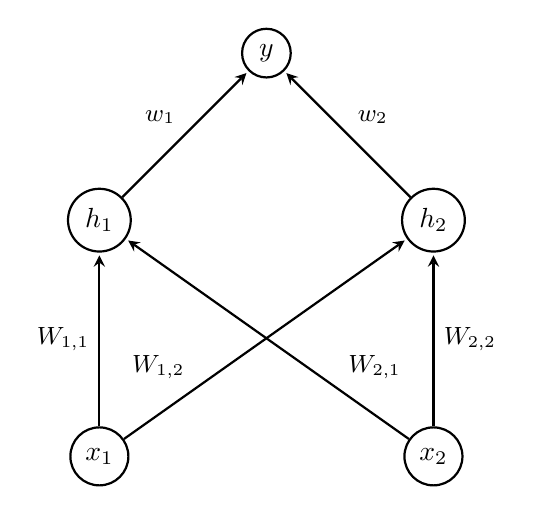
\begin{tikzpicture}[->,>=stealth,shorten >=1pt,auto,node distance=3cm, thick,main node/.style={scale=0.9,circle,draw,font=\sffamily\normalsize}]

            \node[circle, draw] (1)[] {$y$};
            \node[circle, draw] (2)[below left of = 1] {$h_1$};
            \node[circle, draw] (3)[below right of = 1] {$h_2$};
            \node[circle, draw] (4)[below of = 2] {$x_1$};
            \node[circle, draw] (5)[below of = 3] {$x_2$};

            \path[every node/.style={font=\sffamily\small}]
                (2) edge node{$w_1$} (1)
                (3) edge[swap] node{$w_2$} (1)
                (4) edge node{$W_{1,1}$} (2)
                (4) edge[near start] node{$W_{1,2}$} (3)
                (5) edge[swap, near start] node{$W_{2,1}$} (2)
                (5) edge[swap] node{$W_{2,2}$} (3)
                ;
        \end{tikzpicture}
        \caption{The two layer network solving the XOR function on 2 bits.}
    \end{figure}

    The universal approximation theorem tells us that the output layer $y$ must be a linear function. Hence, we set $y = w^Th + b$.
    
    The hidden layer $h$, instead, must use a \curlyquotes{squashing} activation function. Hence, we set $h = \mathrm{ReLU}(W^Tx+c)$, where $\mathrm{ReLU}$ is the \textit{Rectified Linear Unit} function.
    \[\mathrm{ReLU}(z) = \mathrm{max}(0,z) = \soe{ll}{
        z & \text{if } z \geq 0 \\
        0 & \text{if } z < 0
    }\]

    \begin{figure}[H]
        \centering
        \resizebox{0.35\textwidth}{!}{
            \begin{tikzpicture}
                \begin{axis}[%
                    xmax=4, xmin=-4, ymax=6, ymin = -2, domain = -4:4,
                    axis lines = middle
                ]

                \addplot[blue, ultra thick, domain=-4:0] {0};
                \addplot[blue, ultra thick, domain=0:4] {x};
                \end{axis}
            \end{tikzpicture}
        }
        \caption{The Rectified Linear Unit function}
    \end{figure}

    The full model is thus equal to:
    \[y(x) = f(x; \theta) = w^T \mathrm{max}(0, W^Tx+c)+b\]
    with $\theta = \abk{W,c,w,b}$.

    Once the model has been defined, we can now learn the parameters $\theta$ by minimizing the MSE loss function, obtaining that:
    \[W = \smat{1 & 1 \\ 1 & 1} \quad c = \smat{0 \\ 1} \quad w = \smat{1 & -2} \quad b = 0\]

    \begin{figure}[H]
        \centering
        \includegraphics[scale=0.8]{images/xor_space.png}
        \caption{The two feature spaces of the two layers after the learning process.}
    \end{figure}

    The crucial point in the performance of a FNN is its architecture:
    \begin{itemize}
        \item \textit{Depth choice}: how many layers should the network have?
        \item \textit{Width choice}: how many units should each layer of the network have?
        \item \textit{Activation function choice}: which kind of units should each layer have?
        \item \textit{Loss function choice}: which kind of cost function should the network learn on?
    \end{itemize}

    We notice that the universal approximation theorem doesn't say how many units are necessary, but only that a sufficient amount of them is needed. In general, the width of the network tends to be exponential with respect to the size of the input. Moreover, we also notice that, in theory, a short and very wide network can approximate any function. In practice, deep and narrow networks are easier to train and provide better results in generalization.

    \begin{figure}[H]
        \centering
        \includegraphics[scale=0.5]{images/depth_ann.png}

        \includegraphics[scale=0.5]{images/param_ann.png}
        \caption{Relation between depth, number of parameters and accuracy.}
    \end{figure}

    For the choice of activation functions and loss functions, we have to make some remarks regarding the use of gradient-based learning. In particular, we observe that unit saturation can hinder learning. A neuron is said to be saturated when extremely large weights cause the neuron to produce gradient values that are very close to the range boundary. When units saturate, the gradient becomes very small, making lower and lower improvements. To avoid this, we have to choose suitable cost functions and unit non-linearity functions.

    By definition, the FNN model implicitly defines a conditional distribution $\Pr[t \mid x, \theta]$. The loss function that we'll be using is the cross-entropy maximum likelihood principle:
    \[J(\theta) = \Exp_{x,t \sim \mathcal{D}} [-\ln \Pr[t \mid x, \theta]]\]

    where $x,t \sim \mathcal{D}$ denotes the extraction of two random variables $x,t$ from $\mathcal{D}$. Assuming that we have additive Gaussian noise, we know that:
    \[\Pr[t \mid x, \theta] = \mathcal{N}(t \mid f(x; \theta) , \beta^{-1}I)\]

    and thus that:
    \[J(\theta) = \Exp_{x,t \sim \mathcal{D}} \sbk{\frac{1}{2}\mathcal{N}(t \mid f(x; \theta) , \beta^{-1}I)}\]

    In other words, the maximum likelihood estimation with additive Gaussian noise corresponds to the mean squared error minimization.
    
    The choice of the \textbf{output unit activating function} is strictly related to the choice of the cost function. Let $h$ be the output of the last hidden layer, meaning that $y = f^{(n)}(h; \theta)$. Since the universal approximation theorem requires that this activating function is linear, we have a restricted set of choices.
    \begin{itemize}
        \item For \textit{regression}, the identity is chosen as activating function -- meaning that $y = W^Th + b$ -- while the chosen loss functions is the mean squared error (equivalent to maximum likelihood under additive Gaussian noise assumption). In this setup, the output units never saturate due to them being linear.
        
        \item For \textit{binary classification}, the sigmoid is chosen as activating function -- meaning that $y = \sigma(W^Th + b)$ -- while the chosen loss functions is the binary cross entropy, where the likelihood is modeled by a Bernoulli distribution:
        \[J(\theta) = \Exp_{x,t \sim \mathcal{D}} [-\ln \Pr[t \mid x]]\]

        In this setup, the output units saturate only when they give the correct answer.

        \item For \textit{multi-class classification}, the softmax is chosen as activating function
        \[y_i = \mathrm{softmax}(\alpha^{(i)}) = \frac{\exp(\alpha^{(i)})}{\sum_{j \in Y} \exp(\alpha_j)}\]

        where $\alpha^{(i)} = w_i^Th+b_i$, while the chosen loss functions is the categorical cross entropy, where the likelihood is modeled by a multinomial distribution:
        \[J_i(\theta) = \Exp_{x,t \sim \mathcal{D}} [-\ln \mathrm{softmax}(\alpha^{(i)})]\]

        In this setup, the output units saturate only when there are minimal errors.
    \end{itemize}

    For the \textbf{hidden unit activation functions}, instead, we have no theoretical principles, only intuition. In fact, predicting which activation function will work best is usually impossible. Common choices include the rectified linear unit function $\mathrm{ReLU}(\alpha)$, the sigmoid function $\sigma(\alpha)$ and the hyperbolic tangent function $\tanh(\alpha)$. In particular, we observe that the last two are closely related since:
    \[\tanh(\alpha)= 2\sigma(2\alpha)-1\]

    Since none of these functions has a logarithmic term inside them, the units saturate easily. Moreover, gradient based learning is very slow. The hypoerbolic tangent is usually preferred since it gives larger gradients with respect to the sigmoid function.

    \begin{figure}[H]
        \centering
        \resizebox{1\textwidth}{!}{
            \includegraphics{images/ann_2.png}
        }
        \caption{Comparison of the functions and their derivatives. The logit function is the inverse function of the sigmoid.}
    \end{figure}
    
    \section{Backpropagation and learning in ANNs}

    Inside a FNN, information flows forward through the network when computing the output for an input. To train the network, we need to compute the gradients with respect to the network parameters. The usual choice for this task is the \textbf{backpropagation} algorithm, used to propagate gradient computations from the loss function through the whole network. This algorithm makes extensive use of the derivative chain rule -- recall that the network is a sequence of composite functions. We observe that backpropagation isn't a training algorithm: it's just a method to compute the gradient. Moreover, the method isn't specific to FFNs.

    \begin{figure}[H]
        \centering
        \resizebox{0.7\textwidth}{!}{
            \includegraphics[scale=0.5]{images/backprop.png}
        }
        \caption{Visual representation of backpropagation.}
    \end{figure}

    The backpropagation algorithm is divided in two steps: a \texttt{ForwardStep} and a \texttt{BackwardStep}. The former computes the output value of the network and the loss value for that input, while the latter computes the gradient propagating it from the loss value to each layer of the network. The \texttt{ForwardStep} is nothing more than an iterative algorithm that computes the composition of the functions.

    \begin{framedalgo}{Forward step of backpropagation}
        Given the network depth $\ell$, the weight matrices $W^{(1)}, \ldots, W^{(\ell)}$, the bias parameters $b^{(1)}, \ldots, b^{(\ell)}$, the input value $x$ and the target value $t$, the following algorithm computes the output value of the network.

        \begin{algorithmic}
            \Function{ForwardStep}{$\ell, W^{(1)}, \ldots, W^{(\ell)}, b^{(1)}, \ldots, b^{(\ell)}, x, t$}
                \State{$h^{(0)} = x$}
                \For{$k \in [\ell]$}
                    \State{$\alpha^{(k)} = b^{(k)} + W^{(k)} h^{(k-1)}$}
                    \State{$h^{(k)} = f^{(k)}\rbk{\alpha^{(k)}}$}
                \EndFor
                \State{$y = h^{(\ell)}$}
                \State{$J = L(t, y)$} \Comment $L$ is the loss function
                \State{Return $y,J$}
            \EndFunction
        \end{algorithmic}
    \end{framedalgo}

    The \texttt{BackwardStep} is highly based on the vectorial chain rule. Given $y = g(x)$ and $z = f(y) = f(g(x))$, through the chain rule we have that:
    \[\frac{dz}{dx} = \frac{dz}{dy} \frac{dy}{dx}\]

    Similarly, for the vector functions $g : \R^m \to \R^n, f : \R^n \to \R$ we have that:
    \[\frac{\partial z}{\partial x_i} = \sum_{j} \frac{\partial z}{\partial y_j} \frac{\partial y_j}{\partial x_j}\]

    Equivalently, in vector notation we have that:
    \[\nabla_{x} z = \rbk{\frac{\partial y}{\partial x}}^T \nabla_y z\]

    \begin{framedalgo}{Backward step of backpropagation}
        Given the network depth $\ell$, the weight matrices $W^{(1)}, \ldots, W^{(\ell)}$, the bias parameters $b^{(1)}, \ldots, b^{(\ell)}$, the loss value $J$ obtained through the \texttt{ForwardStep}, the following algorithm computes the gradient propagating it from loss function to all the layers of the network.

        \begin{algorithmic}
            \Function{BackwardStep}{$\ell, W^{(1)}, \ldots, W^{(\ell)}, b^{(1)}, \ldots, b^{(\ell)}, J$}
                \State{$g = \nabla_y J$}
                \For{$k = \ell, \ell-1, \ldots, 1$}
                    \State{$g = \nabla_{\alpha^{(k)}} J$, eq. to $g = g \odot f'^{(k)}(\alpha^{(k)})$}
                    \Comment{$\odot$ denotes the element-wise product}
                    \State{$\nabla_{b^{(k)}} J = g$}
                    \State{$\nabla_{W^{(k)}} J = g \cdot (h^{(k-1)})^T$}
                    \State{$g = \nabla_{h^{(k-1)}} J$, eq, to $g = (W^{(k)})^T \cdot g$}
                \EndFor
                \State{Return $g$}
            \EndFunction
        \end{algorithmic}
    \end{framedalgo}

    We notice that the first three instructions inside the for loop of \texttt{BackwardStep} actually propagate the gradients to the pre-nonlinearity activations, while the fourth instruction propagates the gradients to the next lower-level hidden layer.
    
    Suppose that we have a network with a 2D input $x = \smat{x_1 & x_2}$ and two hidden layers $h^{(1)} = \smat{h_1^{(1)} & h_2^{(1)}}$ and $h^{(2)} = \smat{h^{(2)}}$. The last hidden layer is the output layer, hence $y = h^{(2)}$. Let $f^{(1)} = \mathrm{ReLU}$ and $f^{(2)} = \mathrm{id}$.
    
    In the forward step, in order to compute $h^{(1)}, h^{(2)}$ we have to fist compute $\alpha^{(1)} = \smat{\alpha_1^{(1)} & \alpha_2^{(1)}}$ and $\alpha^{(2)} = \smat{\alpha^{2}}$. Since $h^{(0)} = x$, we have that:
    \[\alpha^{(1)} = b^{(1)} + W^{(1)}x = \smat{b_1^{(1)} \\ b_2^{(1)}} + \smat{w_{1,1}^{(1)}x_1 + w_{1,2}^{(1)}x_2 \\ w_{2,1}^{(1)}x_1 + w_{2,2}^{(1)}x_2}\]

    and $h^{(1)} = f^{(1)}(\alpha^{(1)}) = \mathrm{ReLU}(\alpha^{(1)})$. On the second layer, we have that:
    \[\alpha^{(2)} = b^{(2)} + W^{(2)}h^{(1)} = \smat{b^{(1)}} + \smat{w_{1,1}^{(1)}h_1^{(1)} + w_{1,2}^{(1)}h_2^{(1)}}\]

    and $h^{(2)} = f^{(2)}(\alpha^{(2)}) = \alpha^{(2)}$. The loss functions MSE is thus given by:
    \[L(t,y) = \frac{1}{2}(t-y)^2 = \frac{1}{2}(t-\alpha^{(2)})^2\]
    and the parameters of the model are $\theta = \abk{b^{(1)}, b^{(2)}, W^{(1)}, W^{(2)}}$.
    \[b^{(1)} = \smat{b_1^{(1)} \\ b_2^{(1)}} \quad b^{(2)} = \smat{b^{(2)}} \quad W^{(1)} = \smat{w_{1,1}^{(1)} & w_{1,2}^{(1)} \\ w_{2,1}^{(1)} & w_{2,2}^{(1)}} \quad W^{(2)} = \smat{w_{1,1}^{(2)} & w_{1,2}^{(2)}}\]

    This concludes the forward step. To show the correctness of the backward step, we compute the gradients ourself and then show that the algorithm does the same computations in a more efficient way. First, we compute the gradient of the loss function over $y$.
    \[\nabla_y J(\theta) = \frac{\partial J(\theta)}{\partial y} = \frac{\partial}{\partial y} \frac{1}{2}(t-y)^2 = y-t\]

    Using the chain rule, we compute the gradient of the loss function over $b^{(2)}$ and $W^{(2)}$.
    \[\nabla_{b^{(2)}} J(\theta) = \frac{\partial J(\theta)}{\partial y} \frac{\partial y}{\partial b^{(2)}} = \frac{\partial J(\theta)}{\partial y} \cdot 1 = y-t\] 

    \[\nabla_{W^{(2)}} J(\theta) =
    \smat{\frac{\partial J(\theta)}{\partial y} \frac{\partial y}{\partial w_{1,1}^{(2)}} &
    \frac{\partial J(\theta)}{\partial y} \frac{\partial y}{\partial w_{1,2}^{(2)}}} =
    \smat{\frac{\partial J(\theta)}{\partial y} \cdot h_1^{(1)} &
    \frac{\partial J(\theta)}{\partial y} \cdot h_2^{(1)}} = (y-t) (h^{(1)})^T\]

    Similarly, we compute the gradient of the loss function over $h^{(1)}$ and $\alpha^{(1)}$.
    \[\nabla_{h^{(1)}} J(\theta) = \smat{\frac{\partial J(\theta)}{\partial y} \frac{\partial y}{\partial h_{1}^{(1)}} \\ \frac{\partial J(\theta)}{\partial y} \frac{\partial y}{\partial h_{2}^{(1)}}} =  \smat{\frac{\partial J(\theta)}{\partial y} w_{1,1}^{(2)} \\ \frac{\partial J(\theta)}{\partial y} w_{1,2}^{(2)}} = (y-t) (W^{(2)})^T\]

    \[\nabla_{\alpha^{(1)}} J(\theta) = \smat{\frac{\partial J(\theta)}{\partial h_1^{(1)}} \frac{\partial h_1^{(1)}}{\partial \alpha_1^{(1)}} \\ \frac{\partial J(\theta)}{\partial h_2^{(1)}} \frac{\partial h_2^{(1)}}{\partial \alpha_2^{(1)}}} =
    \smat{\frac{\partial J(\theta)}{\partial h_1^{(1)}} \cdot \mathrm{step}(\alpha_1^{(1)}) \\ \frac{\partial J(\theta)}{\partial h_2^{(1)}} \cdot \mathrm{step}(\alpha_2^{1})} = ((y-t) (W^{(2)})^T)\mathrm{step}(\alpha^{(1)})\]

    where $\mathrm{step}$ is the step function, used as the derivative of the ReLU:
    \[\mathrm{step}(x) = \soe{ll}{
        1 & \text{if } x \geq 0 \\
        0 & \text{if } x < 0
    }\]

    \begin{figure}[H]
        \centering
        \resizebox{0.35\textwidth}{!}{
            \begin{tikzpicture}
                \begin{axis}[%
                    xmax=4, xmin=-4, ymax=2, ymin = -2, domain = -4:4,
                    axis lines = middle
                ]

                \addplot[blue, ultra thick, domain=-4:0] {0};
                \addplot[blue, ultra thick, domain=0:4] {1};
                \end{axis}
            \end{tikzpicture}
        }
        \caption{The step function}
    \end{figure}

    Finally, we compute the gradient of the loss function over $b^{(1)}$ and $W^{(1)}$.
    \[\nabla_{b^{(1)}} J(\theta) = \smat{
        \frac{\partial J(\theta)}{\partial \alpha_1^(1)} \frac{\partial \alpha_1^{(1)}}{\partial b_2^{(1)}} \\ \frac{\partial J(\theta)}{\partial \alpha_2^(1)} \frac{\partial \alpha_2^{(1)}}{\partial b_2^{(1)}} 
    } = \smat{
        \frac{\partial J(\theta)}{\partial \alpha_1^(1)} \cdot 1 \\ \frac{\partial J(\theta)}{\partial \alpha_2^(1)} \cdot 1
    } = (y-t) (W^{(2)})^T \odot \mathrm{step}(\alpha^{(1)})\]

    \[\nabla_{W^{1}} J(\theta) = \smat{
        \frac{\partial J(\theta)}{\partial \alpha_1^(1)} \frac{\partial \alpha_1^{(1)}}{\partial w_{1,2}^{(1)}} & \frac{\partial J(\theta)}{\partial \alpha_1^(1)} \frac{\partial \alpha_2^{(1)}}{\partial w_{2,2}^{(1)}} \\
        \frac{\partial J(\theta)}{\partial \alpha_1^(1)} \frac{\partial \alpha_1^{(1)}}{\partial w_{1,2}^{(1)}} & \frac{\partial J(\theta)}{\partial \alpha_2^(1)} \frac{\partial \alpha_2^{(1)}}{\partial w_{2,2}^{(1)}} 
    } = \smat{
        \frac{\partial J(\theta)}{\partial \alpha_1^(1)} \cdot x_1 & \frac{\partial J(\theta)}{\partial \alpha_1^(1)} \cdot x_2 \\
        \frac{\partial J(\theta)}{\partial \alpha_1^(1)} \cdot x_1 & \frac{\partial J(\theta)}{\partial \alpha_2^(1)} \cdot x_2 
    } = ((y-t) (W^{(2)})^T \, \odot \,\mathrm{step}(\alpha^{(1)})) x\]

    By comparing the steps of the algorithm and our calculations, it's easy to see that the backforward algorithm is indeed correct. The Backpropagation algorithm is used inside many training algorithms. In particular, we focus on:
    \begin{itemize}
        \item Stochastic Gradient Descent (SDG)
        \item SGD with momentum
        \item Algorithms with adaptive learning rates
    \end{itemize}

    \begin{framedalgo}{Stochastic Gradient Descent}
        Given a dataset $D$, a learning rate $\eta \geq 0$ and the initial parameters $\theta^{(1)}$, the algorithm computes the gradient descent using the backpropagation and random sampling.

        \begin{algorithmic}
            \Function{StochasticGradientDescent}{$\eta, \theta^{(1)}$}
                \State{$k = 1$}
                \While{the stopping criterion is not met}
                    \State{Randomly sample a minibatch $\{x^{(1)}, \ldots, x^{(m)}\} \subset D$}
                    \State{Compute $g = \frac{1}{m} \nabla_\theta \sum_{i = 1}^m L(f(x^{(i)}, \theta^{(k)}), t^{(i)})$}
                    \Comment{Computed through backprop.}
                    \State{$\theta^{(k+1)} = \theta^{(k)} - \eta g$}
                    \State{$k = k+1$}
                \EndWhile
                \State{Return $\theta^{(k)}$}
            \EndFunction
        \end{algorithmic}
    \end{framedalgo}

    The stopping condition usually used in stochastic gradient descent is a treshold parameter for improvement or a fixed number of iterations. In some advanced models, the hyperparameter $\eta$ changes according to some rule through iterations, where for the first $\tau$ iteration ($k \leq \tau$) we have:
    \[\eta^{(k+1)} = \rbk{1- \frac{k}{\tau}} \eta^{(k)} + \frac{k}{\tau} \eta^{(\tau)}\]
    while for all other iterations $(k > \tau)$ we have $\eta^{(k)} = \eta^{(\tau)}$. This partially removes the overhead of having to find a good static hyperparameter $\eta$ -- the algorithm may diverge if $\eta$ is too large, while it may be too slow if $\eta$ is too small. 

    In SDG with momentum, an additional value called \textbf{momentum} is used to (potentially) accelerate learning. The usefulness of momentum comes in play due to how stochastic gradient can largely vary through the iterations.

    \begin{framedalgo}{SDG with momentum}
        Given a dataset $D$, a learning rate $\eta \geq 0$, a momentum $\mu \in [0,1)$ and the initial parameters $\theta^{(1)}$, the algorithm computes the gradient descent using the backpropagation and random sampling.

        \begin{algorithmic}
            \Function{SDG\_Momentum}{$\eta, \theta^{(1)}$}
                \State{$k = 1$}
                \State{$v^{(1)} = 0$}
                \Comment{$v$ acts as \curlyquotes{velocity}}
                \While{the stopping criterion is not met}
                    \State{Randomly sample a minibatch $\{x^{(1)}, \ldots, x^{(m)}\} \subset D$}
                    \State{Compute $g = \frac{1}{m} \nabla_\theta \sum_{i = 1}^m L(f(x^{(i)}, \theta^{(k)}), t^{(i)})$}
                    \Comment{Computed through backprop.}
                    \State{Compute $v^{(k+1)} = \mu v^{(k)} - \eta g$}
                    \State{$\theta^{(k+1)} = \theta^{(k)} - v^{(k+1)}$}
                    \State{$k = k+1$}
                \EndWhile
                \State{Return $\theta^{(k)}$}
            \EndFunction
        \end{algorithmic}
    \end{framedalgo}

    In some cases, the momentum is applied before computing the gradient. This is variant is called \textbf{Nesterov momentum}. Sometimes, this variant improves the convergence rate.
    \[\overline{\theta} = \theta^{(k)} + \eta v^{(k)}\]
    \[g = \frac{1}{m} \nabla_{\overline{\theta}} L(f(x^{(i)}, \overline{\theta}), t^{(i)})\]

    Other algorithms can have an adaptive learning rate: based on the analysis of the gradient of the loss function it is possible to determine, at any step of the algorithm, whether the learning rate should be increased or decreased. Some examples include:
    \begin{itemize}
        \item AdaGrad
        \item RMSProp
        \item Adam
    \end{itemize}

    As with other ML approaches, regularization is an important feature to reduce overfitting (generalization error). For FNN, we have several options and they can even be applied together:
    \begin{itemize}
        \item \textit{Parameter norm penalties}: we add a regularization term $E_{\mathrm{reg}}$ to the cost function:
        \[E_{\mathrm{reg}}(\theta) = \sum_j \abs{\theta_j}^{q}\]
        \[\overline{J}(\theta) = J(\theta) + \lambda E_{\mathrm{reg}}(\theta)\]
        \item \textit{Dataset augmentation}: we generate additional data and include them in the dataset, usually applying data transformations (e.g. image rotation, scaling, varying illumination conditions, ...) or adding noise.
        \item \textit{Early stopping}: we stop iterations early to avoid overfitting to the training dataset, usually using cross-validation do determine the best iteration to stop on. 
        \item \textit{Parameter sharing}: we impose that the subsets of model parameters are equal. This also improves memory storage.
        \item \textit{Dropout}: we randomly ignore network units with some probability $p$ at each iteration.
    \end{itemize}

    \section{Convolutional Neural Networks}

    \subsection{Convolution}

    Up to now, we treated inputs as general feature vectors. In some cases, inputs have a special structure that can be exploited to get improved results. In general, \textbf{Convolutional Neural Networks (CNN)} work with any type of structure based on \textit{signals}, numerical representations of physical quantities. Deep learning can be directly applied on signals by using suitable operators. In particular, signals have to be represented as a $N$-dimensional \textit{tensor}.
    \begin{itemize}
        \item An audio file is just a variable length 1D vector, i.e. a 1D tensor
        \item An image file is just a multi-channel 2D matrix, i.e. a 3D tensor
        \item A video file is just a sequence of multi-channel 2D matrices sampled through time, i.e. a 4D tensor
    \end{itemize}

    \begin{figure}[H]
        \centering
        \includegraphics[scale=0.6]{images/tensors.png}
        \caption{Tensors with different dimensions.}
    \end{figure}

    CNNs are based on \textbf{convolution}, a mathematical operation on two functions $f,g$ that produces a new function $f * g$. For continuous functions, convolution is defined as the integral of the product of the two functions after one is reflected about the y-axis and shifted. The integral is evaluated for all values of shift, producing the convolution function. The function that gets shifted is called \textbf{kernel} of the convolution. For discrete functions, the same definition holds, but the integral becomes an infinite sum.

    \begin{frameddefn}{Convolution}
        Given two continuous real functions $f, g$, the convolution $f * g$ is defined as:
        \[(f * g)(x) = \int_{-\infty}^{+\infty} f(a) \cdot g(x-a) \, da\]

        For discrete functions, convolutions is defined as:
        \[(f * g)(x) = \sum^{+\infty}_{a = -\infty} f(a) \cdot g(x-a)\]
    \end{frameddefn}

    Another mathematical operation strictly related to convolution is \textbf{cross-correlation}. This operation is similar to convolution, where none of the two functions gets flipped. For this reason, cross-correlation is often known as \textit{sliding dot product}. By manually flipping one of the two functions, cross-comparison can be used to compute convolution.

    \begin{frameddefn}{Cross-correlation}
        Given two continuous real functions $f, g$, the cross-correlation $f \star g$ is defined as:
        \[(f \star g)(x) = \int_{-\infty}^{+\infty} f(x+a) \cdot g(a) \, da\]

        For discrete functions, convolutions is defined as:
        \[(f \star g)(x) = \sum_{a = -\infty}^{+\infty} f(x+a) \cdot g(a)\]
    \end{frameddefn}

    \begin{figure}[H]
        \centering
        \includegraphics[scale=0.3]{images/conv_crosscorr.png}
        \caption{Comparison between correlation and cross-comparison. Convolution is commutative, while cross-comparison is not. }
    \end{figure}

    We observe that cross-correlation is the function that is actually implemented in machine learning libraries, due to it being more efficient to compute through dynamic programming. Since tensors can be viewed as linear applications, convolution and cross-correlation also apply on them. For 2 dimensions, the \textit{limited} discrete 2D convolution of $I$ and $K$ is defined as:
    \[(I * K)(i,j) = \sum_{m \in S_1} \sum_{n \in S_2} I(m,n) K(i-m, j-n)\]
    
    where $S_1,S_2$ are two finite sets -- hence the \textit{limited} in the name of the operation. In other words, during the computation, the kernel slides in both directions.

    \begin{figure}[H]
        \centering
        \includegraphics[scale=0.5]{images/2d_conv.png}
        \caption{Example of 2D convolution of a 2D image and a 2D kernel.}
    \end{figure}

    Similarly, 3D convolution is defined as:
    \[(I * K)(i,j,k) = \sum_{m \in S_1} \sum_{n \in S_2} \sum_{h \in S_3} I(m,n,h) K(i-m, j-n, k-h)\]

    \begin{figure}[H]
        \centering
        \includegraphics[scale=0.6]{images/3d_conv.png}
        \caption{Example of 3D convolution of a 3D image and a 3D kernel.}
    \end{figure}

    We observe that the name 1D/2D/3D convolution \underline{does not} refer to the dimensions of the input and the kernel. Instead, they refer to the number of directions where the kernel slides. For instance, 2D convolutions can be also applied on a 3D input and kernel:
    \[(I * K)(i,j) = \sum_{m \in S_1} \sum_{n \in S_2} \sum_{h \in S_3} I(m,n,h) K(i-m, j-n, h)\]

    \begin{figure}[H]
        \centering
        \includegraphics[scale=0.65]{images/2d_conv_3d.png}
        \caption{Example of computation in 2D convolution of a 3D image and a 3D kernel.}
    \end{figure}

    Convolution can be applied in many ways. To make things simpler, we introduce some terminology to easily describe these processes.
    \begin{itemize}
        \item \textit{Input size}: $(w_{\mathrm{in}} \times h_{\mathrm{in}} \times d_{\mathrm{in}})$ are the dimensions of the input
        \item \textit{Kernel size}: $(w_{\mathrm{k}} \times h_{\mathrm{k}} \times d_{\mathrm{k}})$ are the dimensions of the kernel
        \item \textit{Feature map} (or \textit{Depth slice}): output of the convolution between an input and a kernel
        \item \textit{Depth}: $(d)$ is the number of kernels used
        \item \textit{Padding}: $(p)$ is the number of fillers for outer rows or columns (typically set to 0)
        \item \textit{Stride}: $(s)$ is the number of pixels the kernel moves each time it slides  (when set to 1, no cell of the image is skipped)
        \item \textit{Receptive field}: region in the input space that a particular feature is affected by 
    \end{itemize}

    When the \textbf{multiple kernels} are used, convolution produces multiple feature maps. For instance, if we have an input of size $32 \times 32 \time 1$ and we apply 2D convolution on 1 kernel with dimensions $5 \times 5 \times 1$ kernel, we get a feature map of size $28 \times 28$. Instead, if we apply 6 kernels with dimensions $5 \times 5 \times 3$, each kernel is individually applied on a copy of the input, producing 6 feature maps of size $28 \times 28$. These 6 feature maps are then represented by a $28 \times 28 \times 6$ tensor. In general, if we have an input of size
    \[w_{\mathrm{in}} \times h_{\mathrm{in}} \times d_{\mathrm{in}}\]
    and $d_{\mathrm{out}}$ kernels of size 
    \[w_{\mathrm{k}} \times h_{\mathrm{k}} \times d_{\mathrm{k}}\]
    where $d_\mathrm{k} = \mathrm{in}$, the output will always be a 3D tensor of size
    \[w_{\mathrm{out}} \times h_{\mathrm{out}} \times d_{\mathrm{out}}\]
    where $w_{\mathrm{out}}$ and $h_{\mathrm{out}}$ are computed according to \textit{stride} and \textit{padding} (we'll see how in the next sections). For 3D convolutions, the constraint becomes $d_\mathrm{in} > d_\mathrm{k}$ ad the output is a 4D tensor of size $w_{\mathrm{out}} \times h_{\mathrm{out}} \times z_{\mathrm{out}} \times d_{\mathrm{out}}$,  where $z_{\mathrm{out}}$ is also computed according to \textit{stride} and \textit{padding}.

    \subsection{Convolution in neural networks}

    As the name suggests, CNNs are just FNNs that use convolution in one or more layers. The learning phase finds which kernels are optimal for each layer \textbf{convolutional layer}. Each of these layers is formed by three sub-layers, called \textit{stages}:
    \begin{enumerate}
        \item \textbf{Convolution stage}: application of 2D convolution between input and kernel
        \item \textbf{Detector stage}: application of non-linear activation function on the output of the previous stage
        \item \textbf{Pooling}: reduction in size of the output of the previous stage
    \end{enumerate}

    \begin{figure}[H]
        \centering
        \includegraphics[scale=0.75]{images/conv_layer.png}
        \caption{A convolutional layer.}
    \end{figure}

    The first stage of a convolutional layer applies 2D convolution. We observe that in this stage, 2D convolution is actually applied through cross-correlation:
    \[(I * K)(i,j) = \sum_{m \in S_1} \sum_{n \in S_2} I(i+m, j+n) K(m,n)\]

    This process is very efficient in terms of memory requirements and generalization accuracy, in particular \textbf{sparse connectivity} and \textbf{parameter sharing}. In the former (also called \textit{sparse interactions}), the outputs depend only on a few inputs. In other words, instead of having a completely connected network, we have a sparse network. To achieve this, we use a kernel that is much smaller than input. This property is particularly useful for signals such as images: we expect that each pixel has more influence on other pixels that are close ot it, while far away pixels will be not be influenced by it. In this case, we would prefer a sparse connectivity patter that connects pixels that are close to each other to the same units.

    \begin{figure}[H]
        \centering
        \includegraphics[scale=0.55]{images/sparse_conn.png}
        \caption{Example of a sparse connectivity CNN (top) and a fully connected CNN (bottom). In the former, the input $x_3$ influences a restricted set of units of the next layer.}
    \end{figure}

    In parameter sharing, instead, we learn only one set of parameters (for the kernel) that is shared to all the units. In other words, some weights are shared by all neurons in a particular feature map. This helps to reduce the number of parameters in the whole system, making it computationally cheap.

    \begin{figure}[H]
        \centering
        \includegraphics[scale=0.55]{images/param_share.png}
        \caption{Example of a parameter sharing in CNN (top) and non-parameter sharing (bottom). The black arrows represent the parameters shared by all inputs.}
    \end{figure}

    Another important operation for this stage is \textbf{padding}. This operation controls what happens when the kernel is applied to values that are on the \curlyquotes{border} of the input. For instance, suppose that we have an 1D input of size $32$ and a 1D kernel of size $5$. By applying 1D convolution, we would first apply the kernel to the first $5$ values of the input and then slide by one pixel (assuming stride equal to 1). By repeating this operation for the whole input, we would obtain a 1D feature map of size $28$ (the number of possible slides). In general, if the input has size $w_{\mathrm{in}}$ and the kernel has size $w_{\mathrm{k}}$, we get a feature map of size $w_{\mathrm{in}} - (w_{\mathrm{k}} - 1)$.

    With padding, instead, we extend the \curlyquotes{borders} of the input in order to get more applications of the kernel. In particular, when the padding value $p$ is equal to $\floor{\frac{w_{\mathrm{k}}}{2}}$, the feature map will have the same size of the input. This is called \textit{same padding}. When the padding value $p$ is equal to 0, instead, we say that we have \textit{valid padding} -- due to how only valid applications are done.

    \begin{figure}[H]
        \centering
        \includegraphics[scale=0.55]{images/padding.png}
        \caption{Example of CNN without padding (top) and CNN with padding (bottom).}
    \end{figure}

    The second stage of a convolutional layer, i.e. the \textbf{detector} stage, is nothing more than the traditional application of the activation function of a typical FNN. A more interesting stage is the \textbf{pooling stage}. This stage is in charge of \textit{reducing} the size of the output before feeding it to the next layer. 

    Formally, pooling implements invariance to local translations. When \textit{max pooling} is applied, the stage returns the maximum value of a rectangular region. When \textit{average pooling} is applied, instead, the stage returns the average value of a rectangular region. When applied with a \textit{stride} value larger than 1, the pooling stage reduces the size of the output layer.

    \begin{figure}[H]
        \centering
        \begin{tabular}{ccc}
            \includegraphics[scale=0.55]{images/max_pool.png}
            &\qquad&
            \includegraphics[scale=0.55]{images/downsampling.png}
        \end{tabular}
        \caption{Example of $2 \times 2$ max pooling being applied with stride 2. This stage introduces downsampling as a byproduct.}
    \end{figure}

    Given an input of size $w_{\mathrm{in}} \times h_{\mathrm{in}} \times d_{\mathrm{in}}$, $d_{\mathrm{out}}$ kernels of size $w_{\mathrm{k}} \times h_{\mathrm{k}} \times d_{\mathrm{k}}$, a stride value $s$ and a padding $p$, the dimensions $w_{\mathrm{out}}, h_{\mathrm{out}}$ of the $d_\mathrm{out}$ output feature maps are given by:
    \[w_{\mathrm{out}} = \frac{w_{\mathrm{in}} - w_{\mathrm{k}} + 2p}{s} + 1\]
    \[h_{\mathrm{out}} = \frac{h_{\mathrm{in}} - h_{\mathrm{k}} + 2p}{s} + 1\]
    \[d_{\mathrm{out}} = \text{Number of kernels}\]

    Since the only trainable element in the layer is the kernel, the total number of trainable parameters of the convolutional layer is:
    \[\abs{\theta} = \underbrace{w_{\mathrm{k}} \cdot h_{\mathrm{k}} \cdot  d_{\mathrm{in}} \cdot d_{\mathrm{out}}}_{\text{kernel weights}} + \underbrace{d_{\mathrm{out}}}_{\text{bias}}\]

    By applying these three stages, each convolutional layer inside a CNN applies reduces the size of a single feature map while also increasing the number of such feature maps. In other words, we sequentially trade size for depth until we reach a \textbf{flattened layer}, i.e. a very deep 1D tensor. Once this layer has been reached the network proceeds with a sequence of traditional fully connected layers that classify the extracted flattened layer.

    \begin{figure}[H]
        \centering
        \resizebox{1\textwidth}{!}{
            \includegraphics[scale=0.55]{images/pooling.png}
        }
        \caption{Typical structure of a CNN with multiple convolutional layers.}
    \end{figure}

    The recent success of CNNs is yielded by continuous theoretical advancements in neural networks. However, they also have some downsides: they require massive parallel computing capacities to speed up computations (GPUs/TPUs), very large training sets (ImageNet/MS COCO) and developing frameworks (Keras, Theano, Tensorflow, PyTorch, ...).

    \subsection{Transfer learning}

    Convolutional neural networks are, nowadays, among the most used types of neural network. Over the years, researchers have produced huge datasets (such as ImageNet) that can satisfy the necessity of these models. However, these dataset are clearly specific to some tasks. For new tasks, however, we would require new specific datasets to be created. This bruteforce approach is clearly infeasible: it's impossible to sample a huge dataset for every possible problem. To fix this issue, we use the concept of \textbf{transfer learning}.
    
    Let $D$ be a \textit{domain} defined by datapoints $x_i \in X$ distributed according to $\mathcal{D}(x)$. Let $T$ be a \textit{learning task} defined by labels $y \in Y$, a target function $f : X \to Y$ be a target function and a distribution $P_\mathcal{D}(y \mid x)$.

    Given a target domain $D_T$ and a target learning task $T_T$, we want to improve the learning of $f_T : X_T \to Y_T$ using the knowledge in a source domain $D_S$ and a source learning task $T_S$. In other words, we want to use the training for a source function $f_S : X_S \to Y_S$ to improve the training of a target function $f_T : X_T \to Y_T$.

    In order for this process to work, there must be some intersection between the labels $Y_S, Y_T$ and the inputs $X_S, X_T$. If the intersection is too small, learning capabilities cannot be transferred.

    The first solution for transfer learning is \textbf{fine tuning}. In this case, for the target problem we use the same network architecture of the pre-trained model up to some layer, while also \curlyquotes{copying} their parameters. The copied layers cannot are fixed (\textit{frozen weights}) and they cannot be trained on the new model. To adapt the model for the new task, the last layer of the architecture is usually slightly changed.

    \begin{figure}[H]
        \centering
        \includegraphics[scale=0.7]{images/fine_tuning.png}
        \caption{Example of fine tuning.}
    \end{figure}

    The second solution for transfer learning is \textbf{CNNs as feature extractors}. In this case, we extract the features of a specific layer of the source CNN (usually flattened or dense layers) and then collect the extracted features $x'$ of the training/validation split and associate corresponding labels $t$ in a new dataset $D' = \{(x_i', t_i) \mid i \in [N]\}$. After this process, we train a new classifier $C'$ (another ANN, an SVM, ...) using the dataset $D'$ and classify the extracted features of the test set using $C'$. This process has a huge advantages (there is no need to train a new CNN) but also huge disadvantages (features cannot be modified, hence source and target should be as compatible as possible).

    \chapter{Unsupervised learning}

    \section{K-means}

    In previous chapter, we have strictly focused on supervised learning, i.e. learning methods where the dataset contains a target value for each datapoint. In \textbf{unsupervised learning}, instead, the dataset has no target values. In other words, the dataset is always of the form $D = \{x_i \mid i \in [N]\}$.

    A simple unsupervised learning model is the \textbf{Gaussian Mixture Model (GMM)}. Here, the dataset is generated by a mixed probability distribution is formed by the weighted average of $K$ different gaussian distributions.
    \[\Pr[x] = \sum_{k = 1}^K p_k \mathcal{N}(x; \mu_k, \Sigma_k)\]

    where $p_k, \mu_k$ and $\Sigma_k$ are respectively the prior probability, the mean and the covariance matrix. Each instance $x_i$ of the dataset is generated by:
    \begin{enumerate}
        \item Randomly sample one of the Gaussians according to prior probabilities 
        \item Generate an instance at random according to the chosen Gaussian distribution
    \end{enumerate}

    In this model, the learning phase is reduced to generating such $K$ Gaussians from a dataset in order to produce new samples. To estimate these parameters, we use the \textbf{K-means} algorithm, which computes $K$ means of data generated from $K$ Gaussian distributions.

    \begin{framedalgo}{K-means}
        Given a dataset $D = \{x_i \mid i \in [N]\}$ and a value $K$, the algorithm computes $K$ means for $K$ Gaussian distributions.

        \begin{algorithmic}
            \Function{K-means}{$D, K$}
                \State{Initialize $K$ random centroids for $K$ clusters}
                \Do
                   \State{Assign each $x_i \in D$ to the cluster with the closest centroid}
                   \State{Recompute the centroids of the clusters}
                \doWhile{at least one sample switches cluster}
                \State{Return the $K$ centroids of the clusters.}
            \EndFunction
        \end{algorithmic}
    \end{framedalgo}

    \begin{figure}[H]
        \centering
        \includegraphics[scale=0.9]{images/k_means.png}
        \caption{Execution of the K-means algorithm with $K = 2$}
    \end{figure}

    The convergence of the K-means algorithm will always occur if the following conditions are satisfied:
    \begin{enumerate}
        \item For each switch, the sum of distances from each training sample to that training sample's group centroid is decreased.
        \item There are only finitely many partitions of the training examples into $K$ clusters.
    \end{enumerate}

    \newpage

    We also observe that the K-means algorithm, although simple, has many downsides:
    \begin{itemize}
        \item The choice of the hyperparameter $K$ is critical and must be determined beforehand using intuition
        \item The algorithm is sensitive to initial condition (local optimum) when few data is available
        \item The algorithm is not robust to outliers since data that is very far from may pull the centroids away.
        \item The result is always a circular cluster shape due to it being based on distance
    \end{itemize}

    \section{Estimation Maximization}

    A more advanced algorithm called \textbf{Estimation Maximization (EM)} is capable of not only computing the means of the $K$ Gaussians, but also their covariance matrices and their prior probabilities. Before proceeding, we have to slightly modify our GMM model. In particular, we introduce a new vector $z = \smat{z_1 & \ldots & z_K}^T$ using a 1-out-of-K encoding where $z_k \in \{0,1\}$, where $\Pr[z_k = 1] = p_k$. Thus, we have that:
    \[\Pr[z] = \prod_{k = 1}^K p_k^{z_k}\]

    For a given value $z$, we have that $\Pr[x \mid z_k = 1] = \mathcal{N}(x; \mu_k, \Sigma_k)$. Thus, we get that:
    \[\Pr[x \mid z] = \prod_{k = 1}^K \mathrm{N}(x; \mu_k, \Sigma_k)^{z_k}\]

    Since $z$ is a 1-out-of-K encoding and $\Pr[z_k = 1] = p_k$, using total probability we have
    \[\Pr[x] = \sum_{z} \Pr[z] \Pr[x \mid z] = \sum_{k = 1}^K p_k \mathcal{N}(x; \mu_k, \Sigma_k)\]

    In other words, the GMM distribution $\Pr[x]$ can be seen as the marginalization of a distribution $\Pr[x \mid z]$ over $z$. Given the dataset $D = \{x_i \mid i \in [N]\}$, each datapoint $x_i$ is associated to a corresponding unknown $z_i$, where $z_{i,k} = 1$ if and only if $x_i$ is sampled from the Gaussian $k$. These vectors $z_i$ are called \textbf{latent variables}. Unlike observable variables, which can be directly measured or observed, latent variables represent underlying factors or constructs that are not directly observable but are inferred from other measurable variables.

    For each $z_{i,k}$, we define $\gamma(z_{i,k})$ as:
    \[\gamma(z_{i,k}) = \Pr[z_{i,k} = 1 \mid x_i] = \frac{\Pr[z_{i,k}] = 1 \cdot \Pr[x_i \mid z_{i,k} = 1]}{\Pr[x_i]} = \frac{p_{k} \mathcal{N}(x_i; \mu_k, \Sigma_k)}{\sum_{j = 1}^K p_j \mathcal{N}(x_i; \mu_j, \Sigma_j)}\]

    \begin{figure}[H]
        \centering
        \includegraphics[scale=0.75]{images/gmm.png}
        \caption{(a) $\Pr[x, z]$ with 3 latent variables $z$ (red, gree, blue) -- (b) $\Pr[x]$ marginalized distribution -- (c) $\gamma(z_{i,k})$ posterior distribution}
    \end{figure}

    Consider the maximum likelihood of the GMM:
    \[\argmax_{p, \mu, \Sigma} \ln \Pr[X \mid p, \mu, \Sigma]\]

    The solution of this optimization problem is given by:
    \[p_k = \frac{N_k}{N}\]
    \[\mu_k = \frac{1}{N_k} \sum_{i = 1}^N \gamma(z_{i,k}) x_i\]
    \[\Sigma_k = \frac{1}{N_k} \sum_{i = 1}^N \gamma(z_{i,k}) (x_i - \mu_k)(x_n - \mu_k)^T\]

    where $N_k = \sum_{i = 1}^N \gamma(z_{i,k})$. To efficiently compute these solutions, we use the EM algorithm. This algorithm is divided into two steps: the \textit{Estimation step} and the \textit{Maximization step}. The former computes $\gamma(z_{i,k})$ given current values of $p_k, \mu_k, \Sigma_k$, while the latter computes $p_k, \mu_k, \Sigma_k$ given the current values of $\gamma(z_{i,k})$. By repeatedly applying these operations, the algorithm converges to an estimation of the optimal solution.

    \begin{framedalgo}{Estimation Maximization (EM)}
        Given a dataset $D = \{x_i \mid i \in [N]\}$ and a value $K$, the algorithm computes the means, covariance matrices and prior probabilities for $K$ Gaussian distributions.

        \begin{algorithmic}
            \Function{EM}{$D, K$}
                \State{Initialize $p_k^{(0)}, \mu_k^{(0)}, \Sigma_k^{(0)}$ for each $k \in [K]$}
                \State{Set $t = 0$}
                \While{the terminating condition is not met}
                    \State{Compute the E-Step for each $k \in [K]$ and for each $i \in [N]$:
                    \[\gamma(z_{i,k})^{(t+1)} = \frac{p_{k}^{(t)} \mathcal{N}(x_i; \mu_k^{(t)}, \Sigma_k^{(t)})}{\sum_{j = 1}^K p_j^{(t)} \mathcal{N}(x_i; \mu_j^{(t)}, \Sigma_j^{(t)})}\]}
                    \State{Set $N_k^{(t+1)} = \sum_{i = 1}^{N} \gamma(z_{i,k})^{(t+1)}$}
                    \State{Compute the M-Step for each $k \in [K]$ for each $i \in [N]$:
                    \[p_k^{(t+1)} = \frac{N_k^{(t+1)}}{N} \qquad\qquad \mu_k^{(t+1)} = \frac{1}{N_k^{(t+1)}} \sum_{i = 1}^N \gamma(z_{i,k})^{(t+1)} x_i\]

                    \[\Sigma_k^{(t+1)} = \frac{1}{N_k^{(t+1)}} \sum_{i = 1}^N \gamma(z_{i,k})^{(t+1)} (x_i - \mu_k^{(t+1)})(x_i - \mu_k^{(t+1)})^T\]
                    }
                    \State{Set $t = t+1$}
                \EndWhile

                \State{Return $p_k^{(t)}, \mu_k^{(t)}, \Sigma_k^{(t)}$ for each $k \in [K]$}
            \EndFunction
        \end{algorithmic}
    \end{framedalgo}

    \begin{figure}[H]
        \centering
        \includegraphics[scale=0.7]{images/em.png}
        \caption{Execution of the EM algorithm with $K = 2$.}
    \end{figure}

    The EM algorithm converges to the local maximum likelihood, providing estimates of the latent variables $z_{i,k}$. In some sense, it can be viewed as the extended version of the K-means algorithm, where probabilistic assignments to a cluster $z_{i,k}$.
    
    We also observe that the EM can also be generalized to other distributions. In the general form, we have some observable data $X = \{x_1, \ldots, x_N\}$, some unobserved latent values $Z = \{x_1, \ldots, z_N\}$ and a parametrized probability distribution $\Pr[Y \mid \theta]$ where $Y = \{y_1, \ldots, y_N\}$ is the full data $y_i = \abk{x_i, z_i}$ and $\theta$ are the parameters. The problem asks to determine the optimal parameters $\theta^*$ that locally maximize $\Exp[\ln \Pr[Y \mid \theta]]$. This general version has many uses, in particular in unsupervised clustering, Bayesian networks and Hidden Markov models.

    In its general form, the EM algorithm defines a likelihood function $Q(\theta' \mid \theta)$ on variables $Y = X \cup Z$, using observed $X$ and current parameters $\theta$ to estimate $Z$:
    \begin{enumerate}
        \item In the Estimation step, we compute $Q(\theta' \mid \theta)$ using the current hypothesis $\theta$ and observed data $X$ to estimate the probability distribution over $Y$
        \[Q(\theta' \mid \theta) = \Exp[ \ln \Pr(T \mid \theta') \mid \theta, X]\]
        \item In the Maximization step, we replace the hypothesis $\theta$ with the hypothesis $\theta'$ that maximizes $Q$
        \[\theta := \argmax_{\theta'} Q(\theta' \mid \theta)\]
    \end{enumerate}

    \chapter{Dimensionality reduction}

    \section{Continuous latent variables}

    Consider the following $64 \times 57$ image inside the USPS dataset, representing the digit 6. This image can be mathematically described as an element of the set $\R^{64 \times 57 \times 1}$ -- the last dimension is the number of channels.

    \begin{figure}[H]
        \centering
        \includegraphics[scale=0.4]{images/6_usps.png}
        \caption{Example of a digit image inside the USPS dataset.}
        \label{6_digit}
    \end{figure}
    
    In the data space $\R^{64 \times 57 \times 1}$ of the USPS dataset (or a subset of it), we may have other images with random black pixels. In the context of digit recognitions, images similar to the one below represent no real information. This means that large part of the data space is actually useless.

    \begin{figure}[H]
        \centering
        \includegraphics[scale=0.4]{images/noise.png}
        \caption{Example of another image in the same data space.}
    \end{figure}

    Consider now the dataset formed of all the rotations without translation of the image in \Cref{6_digit}. Each point in this data set is clearly also a point in $\R^{64 \times 57 \times 1}$. However, across this dataset there is only \textbf{one degree of freedom} of variability for the samples, corresponding to the rotation value. This means that the samples of the dataset actually live on a manifold inside $\R^{64 \times 57 \times 1}$ whose \textbf{intrinsic dimensionality} is one. 
    
    In this context, the rotation value is a latent variable since we can observe only the image vectors and we are not told which values of the rotation variable were used to create them. However, we know that the samples in this dataset are somehow related to each other. To get a good representation of this dataset inside the data space, we're interested in finding the best linear transformation from our original data space to a new coordinate system such that the directions, called \textbf{principal components}, capture the largest \textit{variation} in the data and can be easily identified by projecting the samples on the new coordinate system.

    \begin{figure}[H]
        \centering
        \includegraphics[scale=0.9]{images/pca.png}
        \caption{Representation of the dataset projected onto the optimal principal subspace.}
    \end{figure}

    From the figure above, we notice that the rotation dataset assumes a circle-like structure when projected onto the principal subspace. This is actually pretty common for data that has \curlyquotes{structure}, i.e. strong intrinsic relations.

    \newpage

    \section{Principal Components Analysis}

    \textbf{Principal Component Analysis (PCA)} focuses on finding the principal components inside a data that define the optimal \textit{principal subspace}. PCA is used not only for dimensionality reduction, but also for (lossy) data compression, data visualization and feature extraction.

    Given a dataset $D = \{x_i \mid i \in [N]\} \subseteq \R^d$, we want to maximize the data variance after projecting it to some vector $u_1$. In particular, $u_1$ is a unit vector, meaning that $\norm{u} = u_1^Tu_1 = 1$. For each point $x_i \in D$, the projection on $u_1$ is given by $x_i^Tu_1$.
    
    Consider now the mean value of all the data points $\overline{x} = \frac{1}{N} \sum_{i = 1}^N x_i$. We observe that the mean of the projected points is equal to the projection of the mean, i.e. $\overline{x}^T u_1$, while the variance of the projected points is given by:
    \[\frac{1}{N} \sum_{i = 1}^N (u_1^Tx_i - u_1^T \overline{x})^2 = u_1 S u_1\]

    where $S$ is the covariance matrix of the dataset:
    \[S = \frac{1}{N} \sum_{i = 1}^N (x_i - \overline{x_i}) (x_i - \overline{x_i})^T = \frac{1}{N}X^TX\]

    with $X$ being the data-centered matrix of the dataset:
    \[X = \smat{(x_1 - \overline{x})^T \\ \vdots \\ (x_N - \overline{x})^T} \]

    To maximize the projected variance, we have to solve the following optimization problem:
    \[\argmax_{u_1} u_1^T S u_1\]
    subject to $u_1^T u_1 = 1$. Using a Lagrange multiplier $\lambda_1$, this problem is equivalent to the unconstrained maximization of:
    \[\argmax_{u_1} u_1^T S u_1+ \lambda_1 (1-u_1^T u_1)\]

    By setting to zero the derivative with respect to $u_1$ in order to solve the problem, we obtain that:
    \[S u_1 - \lambda_1 u_1 = 0 \implies S u_1 = \lambda_1 u_1\]

    In other words, $u_1$ must be an eigenvector of $S$ and $\lambda_1$ is its eigenvalue. Moreover, using the fact that $u_1^T u_1 = 1$, we also get that:
    \[u_1^T S u_1 = u_1^T \lambda_1 u_1 \implies u_1^T S u_1 = \lambda_1\]

    which is exactly the variance of the samples after the projection. In conclusion, the variance is maximal when $u_1$ is the eigenvector of $S$ corresponding to the largest eigenvalue $\lambda_1$.

    After finding the first principal component $u_1$, if more dimensions are wanted then the whole process can be repeated by picking the next eigenvalues with the largest value in order to obtain the other principal components. In particular, we recall that eigenvectors associated with different eigenvalues are always orthogonal to each other, meaning that the basis $u_1, \ldots, u_m$ produced by applying the process on the $m$ largest eigenvalues is orthonormal.
    
    \begin{framedalgo}{Principal Component Analysis (PCA)}
        Given a dataset $D = \{x_i \mid i \in [N]\} \subseteq \R^d$ and a value $m$, where $m < d$, the algorithm return and orthonormal basis for the principal subspace of dimension $m$.

        \begin{algorithmic}
            \Function{PCA}{$D, m$}
                \State{Compute the mean $\overline{x}$ of $D$}
                \State{Compute the data-centered matrix $X$ of $D$ using $\overline{x}$}
                \State{Compute the covariance matrix matrix $S$ of $D$ using $X$}
                \State{Find the eigenvalues of $S$}
                \State{Find the eigenvectors $u_1, \ldots, u_m$ of the $m$ largest eigenvalues of $S$}
                \State{Return $u_1, \ldots, u_m$}
            \EndFunction
        \end{algorithmic}
    \end{framedalgo}

    Given the principal components $u_1, \ldots, u_m$, the linear transformation that maps each original sample $x_i \in D$ to its representation in the principal subspace is given by:
    \[\phi : D \to \Span(u_1, \ldots, u_m) : x_i \mapsto \smat{x_i^Tu_1 \\ \vdots \\ x_i^T u_m}\]

    We observe that the projection over the new coordinate system looses some information. Hence, if the dimensions chosen for the principal subspace is too small, the dataset will become unusable. To reduce the error, we consider another formulation of the problem. Given the original $d$ dimensional dataset $D$, let $u_1, \ldots, u_d$ be a complete orthonormal base, i.e. such that:
    \[u_j^T u_j = \delta_{i,j} = \soe{ll}{
        1 & \text{if } i = j \\
        0 & \text{otherwise} 
    }\]

    In other words, each vector of the basis has exactly one component set to 1, while all the others are set to 0. No vectors share the same 1-component. Given $x_i \in D$, let $\alpha_1, \ldots, \alpha_d$ be the coefficient of the linear combination of $x_i$ over $u_1, \ldots, u_d$. We notice that:
    \[x_i = \sum_{k = 1}^d \alpha_k u_k = \sum_{k = 1}^d (x_i^T u_k) u_k\]

    Our goal is to approximate $x_i$ using a lower dimensional representation over a restricted subset of $m$ vectors taken from $u_1, \ldots, u_d$.

    For each sample $x_i$, let $\widetilde{x_i}$ be defined as:
    \[\widetilde{x_i} = \sum_{k = 1}^m z_{i,k} u_k + \sum_{h = m+1}^d b_h u_h\]

    where the terms $z_{i,k}$ depend on $x_i$ and the terms $b_h$ are shared among all samples. We evaluate the approximation error using MSE:
    \[J = \frac{1}{N} \sum_{i = 1}^N \norm{x_i - \widetilde{x_i}}^2\]

    Minimizing with respect to $z_{i,k}$ and $b_h$, we get that $z_{i,k} = x_i^T u_k$ for $1 \leq k \leq m$ and $b_h = \widetilde{x_i}^T u_k$. for $m+1 \leq h \leq d$. In other words, for each $x_i$ the best estimation of $\widetilde{x_i}$ is given by the first $m$ components of $x_i$ and the last $d-m$ components shared among all samples. Hence, we get that:
    \[x_i - \widetilde{x_i} = \sum_{h = m+1}^d (x_i^T u_h) u_h + \widetilde{x_i}^T u_h = \sum_{h = m+1}^d ((x_i - \widetilde{x_i}^T)u_h)u_h\]

    meaning that the overall approximation error becomes:
    \[J = \frac{1}{N} \sum_{i = 1}^N  \sum_{h = m+1}^d \norm{x_i - \widetilde{x_i}}^2 (x_i^T u_h - \widetilde{x_i}^T u_h)^2 = \sum_{h = m+1}^d u_h^T S u_h\]

    By minimizing the error using a Lagrange multiplier $\lambda_1$, this problem is equivalent to the unconstrained maximization of:
    \[\argmin_{u_{m+1}, \ldots, u_d} \sum_{h = m+1}^d u_h^T S u_h + \lambda_h(1-u_h^T u_h)\]

    Setting the derivative over $u_h$ to zero for each index, we have that:
    \[S u_h - \lambda_h u_h = 0 \implies S u_h = \lambda_h u_h\]

    meaning that each $u_h$ is the eigenvector of $S$ associated with the eigenvalue $\lambda_h$. Simplifying, we get that:
    \[\argmin_{u_{m+1}, \ldots, u_d} \sum_{h = m+1}^d u_h^T S u_h + \lambda_h(1-u_h^T u_h) = \argmin_{u_{m+1}, \ldots, u_d} \sum_{h = m+1}^d \lambda_h\]
     
    Hence, the principal components $u_{m+1}, \ldots, u_d$ that minimize the error are the eigenvectors associated with the smallest eigenvalues $\lambda_{m+1}, \ldots, \lambda_d$ of $S$ and the approximation error is given by their sum.

    To recap, we have that:
    \begin{itemize}
        \item The $m$ largest eigenvalues of the covariance matrix $S$ of the dataset give the $m$ principal components that maximize the variance of the projections.
        \item The $m$ smallest eigenvalues of the covariance matrix $S$ of the dataset give the $m$ principal components that minimize the error of the projections.
    \end{itemize}

    Instead of computing the full eigenvalue decomposition of $S$ -- a very slow process considering that $d$ may be a huge value --, there are more efficient ways to compute PCA, such as efficient eigenvalue decomposition restricted only $m$ eigenvectors or singular value decompositions of the centered data matrix $X$.

    \begin{figure}[H]
        \centering
        \includegraphics[scale=0.8]{images/pca_2.png}

        \resizebox{1\textwidth}{!}{
            \includegraphics[scale=0.7]{images/pca_3.png}
        }
        \caption{(a) Eigenvalue spectrum and (b) sum of discarded eigenvalues (error)}
    \end{figure}

    If the number of points in the dataset is smaller than the dimensionality of the data space (such as a small set of high resolution images), meaning that $N < d$, at least $d-N+1$ eigenvalues of $S$ are equal to zero, making the process of finding eigenvalues for $S$ very inefficient. To make the process faster, we observe that given $S = \frac{1}{N} X^T X$ the eigenvector equation becomes:
    \[\frac{1}{N}X^TX u_i = \lambda_i u_i\]
    By left-multiplying by $X$, we obtain:
    \[\frac{1}{N}X X^TX u_i = \lambda_i X u_i \implies \frac{1}{N}X X^T v_i = \lambda_i v_i\]

    where $v_i = X u_i$, concluding that $XX^T$ has the same $N-1$ eigenvalues of $X^TX$ (the others are 0). When $N$ is smaller than $d$, the matrix eigenvalues of $XX^T$ can actually be computed more efficiently. After finding the eigenvectors $v_i$ of $XX^T$ of our interest, we notice that by left multiplying by $X^T$ we obtain that:
    \[\frac{1}{N} X^T X X^T v_i = \lambda_i X^T v_i \implies \frac{1}{N}X z_i = \lambda_i z_i\]
    where $z_i =  X^T v_i$, hence $z_i$ is an eigenvector of $S$ with eigenvalue $\lambda_i$. After finding such vectors, we can normalize them by computing:
    \[u_i = \frac{1}{\sqrt{N \lambda_i}} X^T v_i\]

    To summarize, when $N < d$ we can find the eigenvectors with the following procedures:
    \begin{enumerate}
        \item Compute the data-centered matrix $X$
        \item Compute (efficiently) the $N-1$ eigenvalues $\lambda_i$ of $XX^T$
        \item Select the eigenvalues of interest $\lambda_1, \ldots, \lambda_k$ and compute their eigenvectors $v_i, \ldots, v_i$ over $XX^T$
        \item Compute $u_i = \frac{1}{\sqrt{N \lambda_i}} X^T v_i$ to get the eigenvectors for $\lambda_1, \ldots, \lambda_k$ over $S$
    \end{enumerate}

    Another version of PCA can be implemented through probabilities. In this version, we assume that for the vector $x$ of all the $N$ inputs it holds that $x = Wz + \mu$ for some $W,z, \mu$, where $z$ are the lower dimensional latent variables. We also assume Gaussian distribution over $z$ and linear-Gaussian relationship between the latent variables and the data:
    \[\Pr[z] = \mathcal{N}(z; 0,1)\]
    \[\Pr[x \mid z] = \mathcal{N}(x; Wz+\mu, \sigma^2I)\]

    The model parameters in this case become $W, \mu, \sigma$. The marginal distribution is given by:
    \[\Pr[x] = \int_{-\infty}^{+\infty} \Pr[x \mid z] \cdot \Pr[z] \, dz = \mathcal{N}(x; \mu, C)\]

    where $C = WW^T+\sigma^2I$, while the posterior distribution is:
    \[\Pr[z \mid x] = \mathcal{N}(z; M^{-1} W^T(x-\mu), \sigma^2M)\]
    with $M = W^TW+\sigma^2I$. The maximum likelihood for the data $X$ is thus computed through:
    \[\argmax_{W, \mu, \sigma} \ln \Pr[X \mid W, \mu, \sigma^2] = \argmax_{W, \mu, \sigma} \sum_{i = 1}^N \ln \Pr[x_i \mid W, \mu, \sigma^2]\]

    Setting the derivatives to zero, we have the following closed solution for $\mu_{\mathrm{ML}}$:
    \[\mu_{\mathrm{ML}} = \overline{x} = \frac{1}{N} \sum_{i = 1}^N x_i\]

    while $W$ and $\sigma^2$ depend on the eigenvalues and eigenvectors of $S$ (a non-trivial result that we'll be omitting). We observe that this maximum likelihood can also be computed through an algorithm similar to the EM algorithm. 

    \newpage

    \section{Autoencoders}

    An \textbf{autoencoder} is a type of neural network architecture designed to efficiently compress (encode) input data down to its essential features, then reconstruct (decode) the original input from this compressed representation. In other words, an autoencoder can be viewed as the combination of two neural networks, where the former network transforms the input into a low dimensional representation and the latter reconstructs the original input based on reconstruction loss. The usefulness of autoencoders comes from the training process: if the decoder-side of the full network is capable of reconstructing the original data in a good way, then the representation produced by the encoder-side is optimal.

    \begin{figure}[H]
        \centering
        \includegraphics[scale=0.6]{images/autoenc.png}
        \caption{Schematic of an autoencoder.}
    \end{figure}

    Autoencoders are formed by reduced size hidden layers (bottleneck) which learn to reconstruct their input by minimizing a loss function. Given a dataset $D = \{x_i \mid i \in [N]\}$, autoencoders are trained with the same sample $x_i$ used both for input and output. Autoencoders learn ho to encode and decode the samples in a dataset into a low-dimensional space. For this reason, they can also be seen as a method for non-linear principal component analysis.

    \begin{figure}[H]
        \centering
        \includegraphics[scale=0.75]{images/autoenc_2.png}
        \caption{3D reconstruction from the 2D hidden layer generates a 2D manifold in 3D.}
    \end{figure}

    For example, consider an autoencoder for a dataset representing the values $\{0, \ldots, 7\}$, where each value is represented with an 1-out-of-8 encoding, i.e. $4$ is represented as $\smat{0 & 0 & 0& 0& 1 & 0 & 0 & 0}$. A possible autoencoder layout for this dataset is the network formed an input layer with 8 nodes, a hidden layer with 3 nodes and an output layer with 8 nodes. After training, the first layer will have learned how to optimally encode the values $\{0, \ldots, 7\}$ with a 3 dimensional vector.

    Autoencoders are also very useful for anomaly detection, which can be viewed as a binary classification problem $f : X \to \{n, a\}$, where $n$ is the \curlyquotes{normal} class and $a$ is the \curlyquotes{abnormal} class. Using a dataset that contains only normal samples, i.e. $D = \{(x_i, n) \mid \i \in [N]\}$, the autoencoder is capable of predicting if a test $x \in X-X_D$ is normal or abnormal.
    \begin{enumerate}
        \item Train an autoencoder with a dataset $\{x_i \mid i \in [N]\}$ assuming that each sample in the dataset is not abnormal
        \item Compute the final train loss
        \item Determine a treshold $\delta$, such as $\delta = \mathrm{mean}(loss) + \mathrm{std}(loss)$
        \item Given $x' \in X-X_D$, reconstuct $x$ with the autoencoder and compute $\mathrm{loss}'$
        \item If $\mathrm{loss}' < \delta$ return $n$, otherwise return $a$
    \end{enumerate}

    Autoencoders can be based on different learning methods. The most common ones are \textbf{Variational Autoencoders (VAE)}, which focus on learning the latent space structure, and \textbf{Generative Adversarial Networks (GAN)}, which focus on learning a distribution and don't use a latent space.
    
    In VAEs, the goal is to modify data in specific directions, identifying the most meaningful ones for the latent spacae (e.g. \curlyquotes{distort} faces by adding glasses or changin expressions, produce digits from differet hand-writing styles, distort 3D meshes, ...). In other words, we want to feed vectors to the VAE and get a realistic samples of $\Pr[X]$, where $X$ is the sample set. We expect that similar vector values should produce similar generated instances. To achieve this, the encoder produces a distribution instead of an actual encoding, while the decoder operates on sample from this distribution

    \begin{figure}[H]
        \centering
        \includegraphics[scale=0.7]{images/autoenc_3.png}
        \caption{Schematic of Variational Autoencoder (VAE)}
    \end{figure}

    To learn the distribution, the encoder works on a parametric distribution, typically Gaussian, yielding a mean $\mu$ and a covariance matrix $\Sigma$. In the training process, we use a loss term based on Kullback-Leibler divergence.
    \[\mathrm{loss} = \mathrm{MSE} + \mathrm{dKL}(\mathcal{N}(z; \mu, \Sigma), \mathcal{N}(z; 0, I))\]
    
    We also notice that the sampling operation is non differentiable, making backpropagation hard to use. To fix this issue, we add the obtained sample to the backpropagation process (re-parametrization), meaning that the encoder's gradients will also depend on the extracted sample. 

    In GANs, instead, the goal is to produce samples from an input data distribution $\mathcal{X}$. To achieve this, the idea is to invert a neural network (or a CNN if needed). The encoder processes the input and produces a vector, called \textit{code}. The decoder receives a random code and produces an image and reconstructs the image. If the encoder is a CNN, the decoder uses \curlyquotes{deconvolutional layers}, realized through transposed convolution.

    \begin{figure}[H]
        \centering
        \includegraphics[scale=0.6]{images/autoenc_4.png}

        \includegraphics[scale=0.6]{images/autoenc_5.png}
        \caption{Schematic of a Generative Adversarial Networks (GAN)}
    \end{figure}

    To train the decoder, we use \textit{adversarial training}. This training model is based on two or more components that afflict each other: any improvement for one component negatively affects the other components. Eventually, the components will reach a good compromise that maximizes performance. In GAN, adversarial training is realized through a combination of two networks, a generator network (the decoder) and a discriminator network (a critic for the decoder's output).

    \begin{figure}[H]
        \centering
        \includegraphics[scale=0.6]{images/gan.png}
        \caption{Schematic of adversarial training in GANs}
    \end{figure}

    The generator produces samples from the distribution $\Pr[X]$, while the discriminator identifies if a sample actually comes from $\Pr[X]$ or not (the distribution is unknown to the discriminator). To make the two networks compete with each other, the generator tries to fool the discriminator in believing that the sample is correct, while the discriminator tries to separate real samples from the fake ones.
    \begin{enumerate}
        \item Train the discriminator with a batch of data $\{(x_i, \mathrm{real})\} \cup \{x'_j, \mathrm{fake}\}$, where $x_i \in X_D$ and $x_j'$ are images generated from the generator with random values for the latent variables
        \item Train the generator by using the entire model with discriminator layers fixed, i.e. non-trainable, with a batch of data $\{(r_k, \mathrm{real})\}$, where $r_k$ are random values of the latent variable
    \end{enumerate} 

    We observe that the GAN model is actually very powerful. In fact, they can also be used to \textbf{attack} other models. For instance, we can train a GAN model to make it generate images that are slight alterations of a correct image and make the other model believe that it resembles something completely different.

    \begin{figure}[H]
        \centering
        \includegraphics[scale=0.7]{images/gan_adv.png}
        \caption{A GAN is capable of generating adversarial images (bottom) similar to correct one (top) that make another ML model believe they resemble something completely different.}
    \end{figure}

    \chapter{Reinforcement learning}

    \section{Dynamic systems}

    A \textbf{dynamic system} is a system that evolves over time. At any given time $k$, a dynamic system has a \textit{state} $x_k$ representing the current situation of the system.
    The \textit{state transition model} (or \textit{evolution rule}) of the dynamical system is a function $f_k$ that describes what future states follow from the current state $x_k$ and the current state noise $w_k$, i.e. $f_k(x_k, w_k) = x_{k+1}$. The function is often deterministic but in some cases it is also randomized. The system is also provided with an \textit{observation model}, a function $h_k$ that takes in input the current state $x_k$ and the current observation noise $v_k$, returning the current observation $z_k$.

    \begin{figure}[H]
        \centering
        \includegraphics[scale=0.6]{images/dyn_sys.png}
        \caption{A dynamic system.}
    \end{figure}

    Dynamic systems are typically used to predict the future state of a system. In learning, we can use dynamic systems as a prediction tool. In particular, given the past observations $z_0, \ldots, z_k$, we want to learn a model $(f,h)$. In a more formal way, we'll be considering dynamic systems described by:
    \begin{itemize}
        \item A set of states $X$, which can be either an explicite discrete finite representation, a continuous representation or a probabilistic representation
        \item A set of actions $A$, which can be either an explicite discrete finite representation, a continuous representation
        \item A transition function $\delta$, which can be deterministic, non-deterministic or probabilistic
        \item A set of observations $Z$, which can be either an explicite discrete finite representation, a continuous representation or a probabilistic representation
    \end{itemize}

    Each state of a dynamic system encodes all the past knowledge needed to predict the future, all the knowledge gathered through operation and all the knowledge needed to pursue the goal. When the state is fully observable, meaning that the agent is capable of taking an instantanous snapshot of the current state, the decision making problem for an agent is to decide which action must be executed in a given state. In other words, the agent has to compute the function $\pi : X \to A$.

    The dynamic system model fully expresses the concept of \textbf{reinforcement learning}. Differently from supervised and unsupervised learning, in RL we are given a behaviour function $\pi : X \to A$ and a more complex dataset:
    \[D = \{ (x_1,a_1,r_1, \ldots, x_i, a_i, r_i)^{(j)} \mid j \in [N]\}\]

    where each $r_k$ represents the \textbf{reward value} obtained by executing action $a_k$ in state $x_k$. The idea behind reinforcement learning is to make the model learn the optimal strategy that maximizes the total reward value obtain through a \textit{Carrot and Stick Approach}.

    \section{Markov Decision Process}

    A \textbf{Markov Decision Process (MDP)} is any process, i.e. sequence of actions, used for decision making that has the so-called \textit{Markov property}:
    \begin{itemize}
        \item Once the current state is known, the evolution of the dynamic system does not depend on the history of states, actions and observations.
        \item The current state contains all the information needed to predict the future.
        \item Future states are conditionally independent of past states and past observations given the current state.
        \item The knowledge about the current state makes past, present and future observations statistically independent.
    \end{itemize}

    In this simple model, the states are assumed to be fully observable, meaning that we don't need to consider observations obtained through noise.

    \begin{figure}[H]
        \centering
        \resizebox{1\textwidth}{!}{
            \includegraphics[scale=0.6]{images/rl_1.png}
        }
        \caption{Graphical representation of an MDP for salmon fishing.}
    \end{figure}
    
    Formally, MDPs are described as a quadruple $(X,A,\delta,r)$. Depending on the context, the definition of such quadruple changes:
    \begin{itemize}
        \item In an MDP with \textit{deterministic transitions}, $X$ is the set of states, $A$ is the set of actions, $\delta : X \times A \to X$ is a transition function, $r : X \times A \to \R$ is a reward function.
        \item In an MDP with \textit{non-deterministic transitions}, $X$ is the set of states, $A$ is the set of actions, $\delta : X \times A \to \mathcal{P}(X)$ is a transition function, $r : X \times A \times X \to \R$ is a reward function, where the additional state represents the destination state. When action $a$ is executed, the state $x$ transitions to one of the states $x' \in \delta(x,a)$ with equal probability.
        \item In an MDP with \textit{stochastic transitions}, $X$ is the set of states, $A$ is the set of actions, $\delta : X \times A \to \mathcal{P}(X)$ is a transition function, $r : X \times A \times X \to \R$ is a reward function, where the additional state represents the destination state. When action $a$ is executed, the state $x$ transitions to one of the states $x' \in \delta(x,a)$ according to a probability distribution over transitions $\Pr[x' \mid x,a]$.
    \end{itemize}

    In all three cases, the Markov property is enforced by $x_{t+1} = \delta(x_t, a_t)$ and $r_t = r(x_t,a_t)$. In presence of non-deterministic or stochastic actions, the state resulting from the execution of an action is \underline{not known} before the execution of the action, but it can be fully observed \underline{after} its execution.
    
    To give a better intuition behind how these type may vary based on the context, suppose that we want to learn a controller for the grid in \Cref{grid} that reaches the right-most side of the environment from any initial state.
    
    \begin{figure}[H]
        \centering
        \resizebox{0.8\textwidth}{!}{
            \includegraphics[scale=0.6]{images/rl_2.png}
        }
        \caption{Example of a $N \times M$ grid environment with some obstacles.}
        \label{grid}
    \end{figure}

    A deterministic MDP for this problem may be defined as:
    \begin{itemize}
        \item $X = \{(i,j) \mid i \in N, j \in M\}$
        \item $A = \{\mathrm{Left}, \mathrm{Right}, \mathrm{Up}, \mathrm{Down}\}$
        \item $\delta$ : cardinal movements with deterministic effects, i.e. $\delta((i,j), \mathrm{Left}) = (i-1, j)$. if destination state is a black square, the agent remains in the current state.
        \item $r$ : 1000 for reaching the right-most column, -10 for hitting any obstacle, 0 otherwise.
    \end{itemize}
    
    A stochastic MDP for this problem, instead, may be defined as:
    \begin{itemize}
        \item $X = \{(i,j) \mid i \in N, j \in M\}$
        \item $A = \{\mathrm{Left}, \mathrm{Right}\}$
        \item $\delta$ : cardinal movements with probabilistic effects ($0.1$ probability of moving diagonally). If destination state is a black square, the agent remains in the current state.
        \item $r$ : 1000 for reaching the right-most column, -10 for hitting any obstacle, +1 for any $\mathrm{Right}$ action and -1, any $\mathrm{Left}$ action, 0 otherwise.
    \end{itemize}

    \subsection{Optimal policies}

    Given an MDP, we want to find the function $\pi : X \to A$ representing the optimal action to be executed for each state. This function is called \textbf{optimal policy}. The optimality criteria is defined with respect to the expected value of the \textit{cumulative discounted reward} $V^{\pi}(x)$. In the deterministic case, we define:
    \[V^{\pi}(x) = \sum_{i = 1}^{+\infty} \gamma^{i-1} \overline{r_i}\]
    where $\overline{r_i} = r(x_i, a_i, x_{i+1}), a_i = \pi(x_i)$ and $\gamma \in [0,1]$ is the discount factor for future rewards, while in the non-deterministic or stochastic case we define:
    \[V^{\pi}(x) = \Exp \sbk{\sum_{i = 1}^{+\infty} \gamma_{i-1} \overline{r_i}}\]

     The optimal policy is the one that maximizes $V^{\pi}(x)$ over all $x \in X$:
    \[\pi^* \in \argmax_{\pi} V^{\pi}(x) \; \forall x \in X\]

    In other words, we have that $\pi^*$ is an optimal policy if and only if for any other policy $\pi$ it holds that $V^{\pi^*}(x) \geq V^{\pi}(x)$ for all $x \in X$.

    \begin{figure}[H]
        \centering
        \resizebox{0.8\textwidth}{!}{
            \includegraphics[scale=0.6]{images/rl_3.png}
        }
        \caption{Example of optimal policy for the stochastic MDP of the previous example. The green squares represent a $\mathrm{Right}$ action, while the red squares represent a $\mathrm{Left}$ action.}
    \end{figure}

    Figuring out the optimal policy depends entirely on which parts of the MDP are known or not. For instance, if the whole quadruple $(X,A,\delta,r)$ is known, the optimal policy can be found through reasoning or planning. If some parts of the tuple are unknown (typically the reward function), a learning phase is needed.

    To give an example, suppose that we are playing on a bandit with $n$ arms. This machine can be viewed as a one-state MDP $(\{x_0\}, A, \delta, r)$ where $\delta(x_0, a_i) = x_0$ for all $a_i \in A$ and $r : A \to \R$. 

    \begin{figure}[H]
        \centering
        \includegraphics[scale=0.4]{images/rl_4.png}
        \caption{A bandit with 6 arms.}
    \end{figure}

    Since the reward depends only on the arm being pulled, the optimal policy would clearly be the one which always pulls the optimal arm, i.e. the one with maximal reward. To find this policy, we must use different methods based on the situation. When $r$ is deterministic, meaning that each arm will always return the same reward, the solution is given by:
    \[\pi^*(x_0) \in \argmax_{a_i \in A} r(a_i)\]

    If $r$ is also known then $\pi^*(x_0) = a_i^*$, where $r(a_i^*) \geq r(a_j)$ for all $a_j \in A$. If $r$ is unknown, instead, then we can find the optimal policy through $\abs{A}$ iterations: we individually execute each $a_i$ and collect the reward, returning the action that gave the highest reward.

    When $r$ is stochastic (or non-deterministic), meaning that the reward collected by pulling the same arm may change, the solution is given by:
    \[\pi^*(x_0) \in \argmax_{a_i \in A} \Exp[r(a_i)]\]

    If $r$ is also known, the solution is given by $\pi^*(x_0) = a_i^*$, where $a_i^*$ is the action that maximizes the reward value on average based on the distribution of $r$ for $a_i$. For instance, if $r(a_i) = \mathcal{N}(\mu_i, \sigma_i)$ then:
    \[a_i^* \in \argmax_{a_i \in A} \Exp[r(a_i)] = \argmax_{a_i \in A} \mu_i\]

    When $r$ is non-deterministic and unknown, instead, things become more difficult. The typical approach is to use an \textit{online algorithm}, i.e. an algorithm where the input is fed piece-by-piece in a serial fashion instead of having the entire input available from the start.
    
    \begin{enumerate}
        \item Inizialize a data structure $\Theta$
        \item For $t = 1, \ldots, T$ (until termination condition is reached)
        \begin{enumerate}[label={\arabic*.}, start=3]
            \item \textit{Choose} an action $a_{(t)} \in A$
            \item \textit{Execute} $a_{(t)}$ and \textit{collect} the reward $r_{(t)}$
            \item Update $\Theta$ with the collected result 
        \end{enumerate}
    \end{enumerate}
    \begin{enumerate}[label={\arabic*.}, start=6]
        \item Return $\pi^*$ according to how $\Theta$ works
    \end{enumerate}

    The actions written in italics in the above algorithm are executed in an online fashion. Generally, a large number of interactions is needed, meaning that $T \gg \abs{A}$. The way in which the final strategy is chosen strictly depends on the type of data structure used, which also depends on the type of distribution we expect the function $r$ to have. For instance, if $r(a_i) = \mathcal{N}(\mu_i, \sigma_i)$ then the algorithm can be implemented as follows:

    \begin{enumerate}
        \item Inizialize $\Theta_{(0)}[i] = 0$ and $c[i] = 0$ for all $i \in \abs{A}$.
        \item For $t = 1, \ldots, T$ (until termination condition is reached)
        \begin{enumerate}[label={\arabic*.}, start=3]
            \item \textit{Choose} an index $\widehat{i}$ for action $a_{(t)} = a_{\widehat{i}} \in A$
            \item \textit{Execute} $a_{(t)}$ and \textit{collect} the reward $r_{(t)}$
            \item Increment $c[\widehat{i}]$
            \item Update $\Theta_{(t)}[\widehat{i}] = \dfrac{1}{c[\widehat{i}]} (r_{(t)} + (c[\widehat{i}] - 1) \cdot \Theta_{(t-1)}[\widehat{i}])$ 
        \end{enumerate}
    \end{enumerate}
    \begin{enumerate}[label={\arabic*.}, start=6]
        \item Return $\pi^*(x_0) = a_i^*$ with $a_i^* \in \argmax_{a_i \in A} \Theta_{(T)}[i]$
    \end{enumerate}
    
    Given an agent accomplishing a task according to an MDP $⟨X, A, \delta,r⟩$ for which the functions $\delta$ and $r$ are unknown, we want to determine the optimal policy $\pi^*$ that the agent should use. We recall that, differently from supervised learning, in reinforcement learning the dataset has the form:
    \[D = \{ (x_1,a_1,r_1, \ldots, x_i, a_i, r_i)^{(j)} \mid j \in [N]\}\]
    
    Hence, we cannot use samples of the form $(x_{(j)}, \pi(x_{j}))$ in order to learn $\pi^*$. In the general case, to learn a policy we use \textbf{experimentation strategies}. The idea is to explore possible strategies in order to find the actions that maximize the value of a quality function $\widehat{Q}(x,a)$ and then repeat the process on strategies using those actions. We split this process in two phases. In the \textit{exploration phase}, we randomly select an action $a$ (usually with a low value of $\widehat{Q}(x,a)$). In the \textit{exploitation phase}, we select the action $a$ that maximizes $\widehat{Q}(x,a)$.

    The simplest experimentaton strategy is the \textbf{$\mathbf{\varepsilon}$-greedy strategy}: given a value $\varepsilon \in [0,1]$, we select either a random action with probability $\varepsilon$ or the best action with probability $1-\varepsilon$. The $\varepsilon$ value usually decreases over time (exploration followed by exploitation).

    A more advanced experimentation strategy is the \textbf{soft-max strategy}. Actions with higher $\widetilde{Q}$ values are assigned higher probabilities and all actions have at least some probability, i.e. no action has probability zero. For every state $x \in X$ and every action $a_i \in A$, we have that:
    \[\Pr[a_i \mid x] = \frac{k^{\widehat{Q}(x,a_i)}}{\sum_{a_j \in A} k^{\widehat{Q}(x,a_j)}}\]

    where $k > 0$ determines how strongly the selection favors actions with high $\widehat{Q}$ values. The $k$ value usually increases over time (exploration followed by exploitation).

    When $\delta$ and $r$ are unknown, the agent cannot predict the effect of its actions. However, it can still execute them and then observe the outcome. The learning task is thus performed by repeatedly chosing an action, executing it in order to observe the resulting new state and collect its reward.

    There are two main approaches to learning with MDP:
    \begin{itemize}
        \item \textbf{Value iteration} (or \textit{Q-Learning}): estimate $V^*$ and then compute $\pi^*$
        \item \textbf{Policy iteration}: estimate directly $\pi^*$
    \end{itemize}

    \subsection{Value iteration (Q-Learning)}

    In \textbf{value iteration}, the agent could learn the value function $V^{\pi^*}(x)$ (written as $V^*(x)$ for short) from which it could determine the optimal policy through the following formula:
    \[\pi^*(x) \in \argmax_{a \in A} r(x,a) + \gamma V^*(\delta(x,a))\]

    where $\gamma \in [0,1]$ is the discount factor for future rewards. However, since $\delta$ and $r$ are unknown, this policy cannot be directly computed. In the deterministic case, we define the quality function $Q^{\pi}(x,a)$ for a policy $\pi$ as the value we expect to receive when executing $a$ in state $x$ and then acting according to $\pi$. In other words, we have that:
    \[Q^{\pi}(x,a) = r(x,a) + \gamma V^{\pi}(\delta(x,a))\]

    By definition, if the agent learns $Q$, we can determine the optimal policy without knowing $\delta$ and $r$ since:
    \[\pi^*(x) \in \argmax_{a \in A} r(x,a) + \gamma V^*(\delta(x,a)) = \argmax_{a \in A} Q^*(x,a)\]

    We observe that:
    \[V^*(x) = \max_{a \in A} r(x,a) + \gamma V^*(\delta(x,a)) = \max_{a \in A} Q^*(x,a)\]

    Hence, we get that $Q^*(x,a)$ can be defined in terms of itself:
    \[Q^*(x,a) = r(x,a) + \gamma V^{*}(\delta(x,a)) = r(x,a) + \gamma \max_{a' \in A} Q^{*}(\delta(x,a), a')\]

    Let $\widehat{Q}$ be the current approximation of $Q$. The training rule in this case would be:
    \[\widehat{Q}_{(t)}(x,a) = \overline{r} + \gamma \max_{a' \in A} \widehat{Q}_{(t-1)}(x', a')\]

    where $\overline{r} = r(x, a, x')$ is the immediate reward and $x'$ is the state resulting from applying action $a$ to state $x$.

    \begin{framedalgo}{Deterministic Q-Learning}
        Given a deterministic MDP $(X, A, \delta, r)$, the following online algorithm returns an optimal policy $\pi^*$
        \begin{algorithmic}
            \Function{Q\_Learn\_Det}{$X,A, \delta, r$}
                \State For each $x,a$ initialize a table entry $\widehat{Q}_{(0)}(x,a) = 0$
                \State Observe the current state $x$
                \For{$t = 1, \ldots, T$} \Comment{Until termination condition}
                    \State \textit{Choose} a action $a$ 
                    \Comment{According to $\varepsilon$-greedy or soft-max strategy}
                    \State \textit{Execute} the action $a$
                    \State \textit{Observe} the new state $x'$
                    \State \textit{Collect} the immediate reward $\overline{r}$
                    \State Set $\widehat{Q}_{(t)}(x,a) = \overline{r} + \gamma \max_{a' \in A} \widehat{Q}_{(t-1)}(x', a')$ 
                    \State Set $x = x'$
                \EndFor
                \State Return $\pi^*$ defined as $\pi^*(x) \in \argmax_{a \in A} \widehat{Q}_{(T)}(x,a)$
            \EndFunction
        \end{algorithmic}
    \end{framedalgo}

    We observe that for each $t \in [T]$ it holds that $\widehat{Q}_{(t)}(x,a)$ always underestimates $Q^*(x,a)$. In fact, it actually holds that $0 \leq \widehat{Q}_{(t)}(x,a) \leq \widehat{Q}_{(t+1)}(x,a) \leq Q^*(x,a)$. Convergence is guaranteed if all state-actions pares are visited infinitely often.

    To give an example of how the algorithm works, consider a $2 \times 3$ grid of rectangles. Starting from the bottom left square $S_0$, we want to reach the top right square $G$.
    \begin{figure}[H]
        \centering
        \begin{tabular}{|c|c|c|}
            \hline
            $S_3$ & $S_4$ & $G$ \\
            \hline
            $S_0$ & $S_1$ & $S_2$ \\
            \hline
        \end{tabular}
        \caption{The $2 \times 3$ grid}
    \end{figure}
    
    At each time, we can move by one square in any of the four cardinal directions $L, R, U, D$ (only if by moving we're still inside the grid). Each movement has an associated reward value: if we move from a different square to the goal square we get 100 points, otherwise we get 0 points. 
    
    \begin{figure}[H]
        \centering

        \begin{tikzpicture}[->,>=stealth,shorten >=1pt,auto,node distance=3cm, thick,main node/.style={scale=0.9,circle,draw,font=\sffamily\normalsize}]

            \node[state] (0)[]{$S_3$};
            \node[state] (1)[right of = 0]{$S_4$};
            \node[state] (2)[right of = 1]{$G$};
            \node[initial, state] (3)[below of = 0]{$S_0$};
            \node[state] (4)[right of = 3]{$S_1$};
            \node[state] (5)[right of = 4]{$S_2$};

            \path[every node/.style={font=\sffamily\small}]
                    (0) edge[bend left] node{0} (1)
                    (0) edge[bend left] node{0} (3)

                    (1) edge[bend left] node{0} (0)
                    (1) edge[] node{100} (2)
                    (1) edge[bend left] node{0} (4)

                    (2) edge[loop right] node{0} (2)

                    (3) edge[bend left] node{0} (0)
                    (3) edge[bend left] node{0} (4)

                    (4) edge[bend left] node{0} (3)
                    (4) edge[bend left] node{0} (1)
                    (4) edge[bend left] node{0} (5)

                    (5) edge[] node{100} (2)
                    (5) edge[bend left] node{0} (4)
                ;
        \end{tikzpicture}
        \caption{Deterministic MDP describing the grid goal problem.}
    \end{figure}

    Here, the value function $V^*$ of the optimal policy assumes the following values:
    \begin{figure}[H]
        \centering
        \begin{tabular}{c | c c c c c c}
            $\mathbf{x}$ & $S_0$ & $S_1$ & $S_2$ & $S_3$ & $S_4$ & $G$ \\
            \hline
            $\mathbf{V^*(x)}$ & $81$ & $90$ & $100$ & $90$ & $100$ & $0$
        \end{tabular}
    \end{figure}

    After the training process, the $\widehat{Q}$ converges to values very close to the optimal ones: 

    \begin{figure}[H]
        \centering

        \begin{tikzpicture}[->,>=stealth,shorten >=1pt,auto,node distance=3cm, thick,main node/.style={scale=0.9,circle,draw,font=\sffamily\normalsize}]

            \node[state] (0)[]{$S_3$};
            \node[state] (1)[right of = 0]{$S_4$};
            \node[state] (2)[right of = 1]{$G$};
            \node[initial, state] (3)[below of = 0]{$S_0$};
            \node[state] (4)[right of = 3]{$S_1$};
            \node[state] (5)[right of = 4]{$S_2$};

            \path[every node/.style={font=\sffamily\small}]
                    (0) edge[bend left, color=red] node{90} (1)
                    (0) edge[bend left] node{72.9} (3)

                    (1) edge[bend left] node{81} (0)
                    (1) edge[color=red] node{100} (2)
                    (1) edge[bend left] node{81} (4)

                    (2) edge[loop right, color=red] node{0} (2)

                    (3) edge[bend left] node{81} (0)
                    (3) edge[bend left, color=red] node{81} (4)

                    (4) edge[bend left] node{72.9} (3)
                    (4) edge[bend left] node{90} (1)
                    (4) edge[bend left, color=red] node{90} (5)

                    (5) edge[color=red] node{100} (2)
                    (5) edge[bend left] node{81} (4)
                ;
        \end{tikzpicture}
        \caption{Values learned through the deterministic $Q$ learning process. The red arrows represent the optimal policy returned by the algorithm.}
    \end{figure}

    The evaluation of RL agents is usually performed through cumulative reward gained over time. Due to the various exploration phases that the algorithm may take, the  cumulative reward plot may be very noisy. A better approach could involve the repeated execution (until termination condition) of $k$ steps of learning followed by an evaluation of the current learned policy.

    \begin{figure}[H]
        \centering
        \includegraphics[scale=0.85]{images/cum_rew.png}
        \caption{Cumulative reward plot of an RL agent learning phase.}
    \end{figure}
    
    In the stochastic (or non-deterministic) case, the deterministic Q-Learning algorithm is not guaranteed to converge due to $\widehat{Q}_{(t)}(x,a) \leq \widehat{Q}_{(t+1)}(x,a)$ not always being true. Hence, we have to use a new training rule. First, we recall that the value function $V^{\pi}(x)$ is defined in terms of expected value. Hence, we define $Q^{\pi}$ as:
    \[Q^{\pi}(x,a) = \Exp[r(x,a) + \gamma V^{\pi}(\delta(x,a))]\]

    Similarly to the deterministic case, we get that:
    \[\begin{split}
        Q^*(\pi)(x,a) &= \Exp[r(x,a) + \gamma V^{*}(\delta(x,a))] \\
        &= \Exp[r(x,a)] + \gamma \Exp[V^{*}(\delta(x,a))] \\
        &= \Exp[r(x,a)] + \gamma \sum_{x' \in X} \Pr[x' \mid x,a] \cdot V^*(x') \\
        &= \Exp[r(x,a)] + \gamma \sum_{x' \in X} \Pr[x' \mid x,a] \cdot \max_{a' \in A} Q^*(x',a')\\
    \end{split}\]

    While the training rule is adapted as:
    \[\begin{split}
        \widehat{Q}_{(t)}(x,a) &= \widehat{Q}_{(t-1)}(x, a) + \alpha_{(t-1)}(\overline{r} + \gamma \max_{a' \in A} (\widehat{Q}_{(t-1)}(x', a')) - \widehat{Q}_{(t-1)}(x, a)) \\
        &= (1-\alpha_{(t-1)}) \widehat{Q}_{(t-1)}(x, a) + \alpha(\overline{r} + \gamma \max_{a' \in A} \widehat{Q}_{(t-1)}(x', a'))
    \end{split}\]

    where $\alpha_{(t-1)} = \frac{1}{1+v_{(t-1)}(x,a)}$, with $v_{(t-1)}(x,a)$ being the total number of times the state-action pair $(x,a)$ has been visited up to the $t$-th iteration. Through this rule, the non-deterministic Q-Learning algorithm is guaranteed to converge when every pair state-action is visited infinitely often.

    \begin{figure}[H]
        \centering

        \begin{tikzpicture}[->,>=stealth,shorten >=1pt,auto,node distance=3cm, thick,main node/.style={scale=0.9,circle,draw,font=\sffamily\normalsize}]

            \node[state] (0)[]{$S_3$};
            \node[state] (1)[right of = 0]{$S_4$};
            \node[state] (2)[right of = 1]{$G$};
            \node[initial, state] (3)[below of = 0]{$S_0$};
            \node[state] (4)[right of = 3]{$S_1$};
            \node[state] (5)[right of = 4]{$S_2$};

            \path[every node/.style={font=\sffamily\small}]
                    (0) edge[bend left] node{0} (1)
                    (0) edge[bend left] node{0} (3)
                    (0) edge[out = 60, in = 120] node{100} (2)

                    (1) edge[bend left] node{0} (0)
                    (1) edge[] node{100} (2)
                    (1) edge[bend left] node{0} (4)

                    (2) edge[loop right] node{0} (2)

                    (3) edge[bend left] node{0} (0)
                    (3) edge[bend left] node{0} (4)
                    (3) edge[out = 300, in = 240] node{0} (5)

                    (4) edge[bend left] node{0} (3)
                    (4) edge[bend left] node{0} (1)
                    (4) edge[bend left] node{0} (5)

                    (5) edge[] node{100} (2)
                    (5) edge[bend left] node{0} (4)
                ;
        \end{tikzpicture}
        \caption{Non-deterministic MDP describing the grid goal problem where we're also allowed to move right by two squares.}
    \end{figure}

    For non-deterministic learning there are also more advanced Q-Learning algorithm: the TD algorithm and the SARSA algorithm. \textbf{Temporal difference (TD)} Q-learning is a variant of Q-learning where the discrepancy between successive Q estimates reduces over time. Given a value $n$, the $n$ step time difference of the function Q is given by:
    \[\widehat{Q}^{*^{(n)}}(x_t,a_t) = \overline{r}_{t} + \gamma \overline{r}_{t+1} + \gamma^{n-1}\overline{r}_{t+n-1} + \gamma^n \max_{a' \in A} \widehat{Q}(x_{t+n}, a')\]

    Given a value $\lambda \in [0,1]$, we define:
    \[Q^\lambda(x_t,a_t) = (1-\lambda) \sum_{i = 1}^{+\infty} \lambda^{i-1}Q^{*^{(i)}}(x_t, a_t)\]

    which is equivalent to:
    \[Q^\lambda(x_t,a_t) = r_t + \gamma ((1-\lambda) \max_{a' \in A} \widehat{Q}(x_t,a_t) + \lambda Q^{\lambda}(x_{t+1}, a_{t+1}))\]

    We observe that:
    \begin{itemize}
        \item When $\lambda = 0$, we have that $Q^\lambda(x_t,a_t) = \widehat{Q}^{*^{(1)}}(x_t,a_t)$
        \item When $\lambda = 1$, only observed $r_{t+1}$ are considered
        \item When $0 < \lambda < 1$, the algorithm increases the emphasis on discrepancies based on more distant look-aheads
    \end{itemize}

    The $TD(\lambda)$ algorithm uses the above training rule, which sometimes converges faster than standard Q-Learning. Moreover, it is guaranteed to converge $\lambda \in [0,1]$ for learning $V^*$.
    
    In \textbf{SARSA} Q-learning, instead, we use a tuple $(s,a,r,s',a')$ (equivalent to $(x,a,r,x',a')$ in our notation) in order to define:
    \[\widehat{Q}_{(t)}(x,a) = \widehat{Q}_{(t-1)}(x,a) + \alpha(\overline{r} + \gamma \widehat{Q}_{(t-1)}(x',a') - \widehat{Q}_{(t-1)}(x,a))\]
    where $x',a'$ are chosen accordingly to a policy based on current estimate of $Q$

    \begin{figure}[H]
        \centering
        \includegraphics[scale=0.75]{images/rl_5.png}
        \caption{Comparison of the non-deterministic Q-Learning variants.}
    \end{figure}

    We observe that, in all variants, an explicit representation of $\widehat{Q}$ through a table may not be feasible for large models. In this case, we define an approximating function $Q_\theta(x,a) = \theta_0 + \theta_1 F_1(x,a) + \ldots + \theta_n F_n(x,a)$ and use a linear regression to learn it, usually through a neural network.

    \subsection{Policy iteration}

    In \textbf{policy iteration} we directly estimate the optimal policy $\pi$ instead of estimanting the functions $V$ and $Q$. Each policy can be parametricly represented as:
    \[\pi_\theta(x) = \max_{a \in A} \widehat{Q}_\theta(x,a)\]

    Let $\rho(\theta)$, called \textit{policy value}, be the expected value of executing $\pi_\theta$. The policy gradient is given by $\nabla_\theta \rho(\theta)$. In its generic form, the policy gradient algorithm for a parametric representation of the policy $\pi_\theta(x)$ corresponds to:
    \begin{enumerate}
        \item Choose $\theta$
        \item Repeat until terminating condition: estimate $\nabla_\theta \rho(\theta)$ through experiments and set $\theta := \theta + \eta \nabla_\theta \rho(\theta)$
    \end{enumerate}

    In robot learning, we use a more refined approach:
    \begin{enumerate}
        \item Let $\pi$ be an initial policy
        \item Repeat until terminating condition: compute $t$ random perturbations of $\pi$  $R_1, \ldots, R_k$ and set $\pi$ as the best combination of $R_1, \ldots, R_k$
    \end{enumerate}

    The perturbations are generated from $\pi$ by setting $R_i = \{\theta_1 + \delta_1, \ldots, \theta_N + \delta_N\}$, with $\delta_i$ being randomly chosed from $\{-\varepsilon_j, 0, +\varepsilon_j\}$ for some small fixed value $\varepsilon_j$ relative to $\theta_j$.
    The last step is usually problem-specific. In the eastiest case, we set 
    \[\pi \in \argmax_{j \in [k]} F(R_j)\]
    for some evaluation function $F$. For more complex cases, we combine $R_1, \ldots, R_t$ by setting:
    \[\pi := \pi + \frac{A}{\abs{A}} \eta\]

    with:
    \[A_j = \soe{ll}{
        0 & \text{if } \mathrm{Avg}_{0,j} > \mathrm{Avg}_{-\varepsilon,j} \text{ and } \mathrm{Avg}_{0,j} > \mathrm{Avg}_{+\varepsilon,j} \\
        \mathrm{Avg}_{+\varepsilon,j} - \mathrm{Avg}_{-\varepsilon,j} & \text{otherwise}
    }\]

    and where:
    \begin{itemize}
        \item $\mathrm{Avg}_{-\varepsilon, j}$ is the average score of all $R_i$ with a negative perturbation
        \item $\mathrm{Avg}_{0, j}$ is the average score of all $R_i$ with a zero perturbations
        \item $\mathrm{Avg}_{+\varepsilon, j}$ is the average score of all $R_i$ with a positive perturbation
    \end{itemize}

    \section{Hidden Markov Model} 

    In some cases, even the actions of a Markov Decision Process may be unknown. When this happens, the stochastic MDP model becomes equivalent to a \textbf{Markov Chain}, a dynamic system evolving according to the Markov property where future evolutions depend only on the current state $x_t$ instead of a pair $(x_t,a_t)$. In other words, Markov chains can be seen as a stochastic MDP where there is only one action that can be executed.

    A \textbf{Hidden Markov Model (HMM)} is a triple $(X,Z,\pi_0)$ where $X$ is a finite set of discrete states that are non-observable in a direct way, $Z$ is a set of observations that can be discrete or continuous and $\pi_0$ is an initial distribution. Each state $x_t$ assumes a hidden value (hence the non-observability) and it can stochastically transition to the state $x_{t+1}$. Moreover, each state $x_t$ can stochastically produce an observation $z_t$. Since the states cannot be observed directly, the goal is to learn the current state by observing the current observation.
    
    The transition model and observation model are governed by $\Pr[x_t \mid x_{t-1}]$ and $\Pr[z_t \mid x_t]$. For each state, a \textit{state transition matrix} $A$ determines the transition probabilities for the values assumed by $x_t$ and $x_{t+1}$:
    \[a_{i,j} = \Pr[x_t = j \mid x_{t-1} = i]\]

    Similarly, the observation model is described by a function $b_k$ for each value $k$ where:
    \[b_k(z_t) = \Pr[z_t \mid x_t = k]\]

    The initial probability distribution always corresponds to $\pi_0 = \Pr[x_0]$.

    \begin{figure}[H]
        \centering

        \begin{tikzpicture}[->,>=stealth,shorten >=1pt,auto,node distance=3cm, thick,main node/.style={scale=0.9,circle,draw,font=\sffamily\normalsize}]

            \node[initial, rectangle, draw, rounded corners] (0)[]{$x_1 \in I$};
            \node[rectangle, draw, rounded corners] (1)[right of = 0]{$x_2 \in I$};
            \node[rectangle, draw, rounded corners] (2)[right of = 1]{$x_3 \in I$};
            \node[rectangle, draw, rounded corners] (3)[right of = 2]{$x_4 \in I$};
            \node[rectangle, draw, rounded corners] (4)[right of = 3]{$x_5 \in I$};

            \node[rectangle, draw, rounded corners] (5)[below of = 0]{$z_1 \in O$};
            \node[rectangle, draw, rounded corners] (6)[right of = 5]{$z_2 \in O$};
            \node[rectangle, draw, rounded corners] (7)[right of = 6]{$z_3 \in O$};
            \node[rectangle, draw, rounded corners] (8)[right of = 7]{$z_4 \in O$};
            \node[rectangle, draw, rounded corners] (9)[right of = 8]{$z_5 \in O$};

            \path[every node/.style={font=\sffamily\small}]
                    (0) edge node{$p_1$}(1)
                    (1) edge node{$p_2$}(2)
                    (2) edge node{$p_3$}(3)
                    (3) edge node{$p_4$}(4)

                    (0) edge node{$q_1$}(5)
                    (1) edge node{$q_2$}(6)
                    (2) edge node{$q_3$}(7)
                    (3) edge node{$q_4$}(8)
                    (4) edge node{$q_5$}(9)
                ;
        \end{tikzpicture}
        \caption{Example of a HMM. The set $I$ is discrete, while the set $O$ can be either discrete or continuous. For each $i$ we have that $p_i = \Pr[x_{i+1} = a \mid x_i = b]$ and $q_i = \Pr[z_t \mid x_i = a]$}
    \end{figure}

    HMMs are typically used for status recognition. For instance, a sensor may recognize the currently unknown status of the stoplight (discrete set of states) only through photos of a traffic light (continuous set of multi-dimensional observations).

    To infer on HMMs, we work with one of two setups:
    \begin{itemize}
        \item \textbf{Filtering}: we assume that
        \[\Pr[x_T = k \mid z_{1:T}] = \frac{\alpha_T^k}{\sum_{j} \alpha_T^j}\]
        \item \textbf{Smoothing}: we assume that
        \[\Pr[x_T = k \mid z_{1:T}] = \frac{\alpha_T^k \beta_T^k}{\sum_{j} \alpha_T^j \beta_T^j}\]
    \end{itemize}
    where $x_T$ is the last state, $\alpha_t^k = \Pr[x_t = k, z_{1:t}]$ and $\beta_t^k = \Pr[z_{t:T} \mid x_t = k]$. The application of the chain rule on HMMs allows us to factorize the entire model through a single probability that expresses it:
    \[\Pr[x_{0:T}, z_{1:T}] = \Pr[x_0] \cdot \Pr[z_0 \mid x_0] \cdot \Pr[x_1 \mid x_0] \cdot \ldots \cdot \Pr[z_{T-1} \mid x_{T-1}] \cdot \Pr[x_T \mid x_{T-1}]\]

    This allows us to stochastically compute the values assumed by the states starting from $\Pr[x_T = k \mid z_{1:T}]$ and by computing $\alpha_t^k, \beta_t^k$ for each $t \in [T]$. To achieve this, we split the process in two steps In the \textit{forward step}, we compute $\alpha_t^k$ using the following procedure:
    \begin{enumerate}
        \item For each state $k$ let:
        \[\alpha_0^k = \pi_0 b_k(z_0)\]
        \item For each $t = 1, \ldots, T$ and each state $k$ let:
        \[\alpha_t^k = b_k(z_t) \sum_{j} \alpha^i_{t-1} a_{i,k}\]
    \end{enumerate}

    \textit{Note}: recall that $a_{i,k} = \Pr[x_t = k \mid x_{t-1} = i]$ and $b_k(z_t) = \Pr[z_t \mid x_t = k]$.
    
    In the \textit{backward step}, we compute $\beta_t^k$ in a similar way:
    \begin{enumerate}
        \item For each state $k$ let:
        \[\beta_T^k = 1\]
        \item For each $t = T-1, \ldots, 1$ and each state $k$ let:
        \[\beta_t^k = \sum_{j} \beta^i_{t+1} a_{k,j} b_j(z_{t+1}) \]
    \end{enumerate}

    During the learning phase, given the output sequences we want to determine the maximum lihelihood estimate of the parameters of the HMM (transmission and emission probabilities). If the states can be observed at training time, the transition and observation models can be estimated with statistical analysis by setting:
    \[a_{i,j} = \Pr[x_t = j \mid x_{t-1} = i] = \frac{\abs{\{i \to j \text{ transitions}\}}}{\abs{\{i \to * \text{ transitions}\}}}\]
    \[b_k(z) =  \Pr[z_t \mid x_t = k] = \frac{\abs{\{\text{observe $z$ in state $k$}\}}}{\abs{\{\text{observe $*$ in state $k$}\}}}\]

    If the states cannot be observed even in the training phase, we compute a local maximum likelihood using a variant of the EM algorithm.

    \section{Partially Observable MDP}

    A \textbf{Partially Observable MDP (POMDP)} is a generalization of the MDP model where the agent's decision process assumes that the system dynamics are determined by an MDP, but the agent cannot directly observe the underlying state. In other words, a POMDP combines the decision making of MDP and the non-observability of HMM.

    A POMDP is a quintuple $(X,A,Z,\delta,r,o)$ where:
    \begin{itemize}
        \item $X$ is a set of states
        \item $A$ is a set of actions
        \item $Z$ is a set of observations
        \item $P[x_0]$ is a probability distribution of the initial state
        \item $\delta(x,a,x') = \Pr[x' \mid x,a]$ is a probability distribution over transitions
        \item $r(x,a)$ is a reward function
        \item $o(x',a,z') = \Pr[z' \mid x',a]$ is a probability distribution over observations
    \end{itemize}

    \begin{figure}[H]
        \centering

        \begin{tikzpicture}[->,>=stealth,shorten >=1pt,auto,node distance=3cm, thick,main node/.style={scale=0.9,circle,draw,font=\sffamily\normalsize}]

            \node[initial, rectangle, draw, rounded corners] (0)[]{$x_1 \in I$};
            \node[rectangle, draw, rounded corners] (1)[right of = 0]{$x_2 \in I$};
            \node[rectangle, draw, rounded corners] (2)[right of = 1]{$x_3 \in I$};
            \node[rectangle, draw, rounded corners] (3)[right of = 2]{$x_4 \in I$};
            \node[rectangle, draw, rounded corners] (4)[right of = 3]{$x_5 \in I$};

            \node[rectangle, draw, rounded corners] (5)[below of = 0]{$z_1 \in O$};
            \node[rectangle, draw, rounded corners] (6)[right of = 5]{$z_2 \in O$};
            \node[rectangle, draw, rounded corners] (7)[right of = 6]{$z_3 \in O$};
            \node[rectangle, draw, rounded corners] (8)[right of = 7]{$z_4 \in O$};
            \node[rectangle, draw, rounded corners] (9)[right of = 8]{$z_5 \in O$};

            \node[state] (10)[above of = 0]{$a_1$};
            \node[state] (11)[right of = 10]{$a_2$};
            \node[state] (12)[right of = 11]{$a_3$};
            \node[state] (13)[right of = 12]{$a_4$};

            \path[every node/.style={font=\sffamily\small}]
                    (0) edge node{$p_1$}(1)
                    (1) edge node{$p_2$}(2)
                    (2) edge node{$p_3$}(3)
                    (3) edge node{$p_4$}(4)

                    (0) edge node{$q_1$}(5)
                    (1) edge node{$q_2$}(6)
                    (2) edge node{$q_3$}(7)
                    (3) edge node{$q_4$}(8)
                    (4) edge node{$q_5$}(9)
                    
                    (10) edge node{$h_1$}(1)
                    (11) edge node{$h_2$}(2)
                    (12) edge node{$h_3$}(3)
                    (13) edge node{$h_4$}(4)
                ;
        \end{tikzpicture}
        \caption{Example of a POMDP.}
    \end{figure}

    As per standard MDPs, we want to find an optimal policy that the agent can use. A trivial solution is to define the policy using a history of observations-action pairs. To achieve this, we would need a long history in order to correctly estimate the probabilities. The state-of-the-art solution is to use \textbf{belief states}, a set of possible states the process may be in. Let $b(x)$ be a probability distribution over the states. A POMDP can be described as an MDP $(B,A,\tau,\rho)$ where:
    \begin{itemize}
        \item $B$ is an infinite set of belief states
        \item $A$ is a set of actions
        \item $\tau(b,a,b')$ is a probability distribution over transitions
        \item $\rho(b,a,b')$ is a reward function
    \end{itemize}

    In this context, we want to get the optimal policy $\pi^* : B \to A$. Given a current belief state $b$, an action $a$ and an observation $z'$ obtained after the execution of $a$, let $\mathrm{SE}(b,a,z')$ be a state-estimating function whose output is the next belief state $b'(x')$. Through some manipulation, we obtain that:
    \[\begin{split}
        b'(x') &= \mathrm{SE}(b,a,z') \\
        &= \Pr[x' \mid b,a,z'] \\
        &= \frac{\Pr[z' \mid x',b,a] \cdot \Pr[x' \mid b,a]}{\Pr[z' \mid b,a]} \\
        &= \frac{\Pr[z' \mid x',b,a] \cdot \sum_{x \in X} \Pr[x' \mid b,a,x] \cdot \Pr \Pr[x \mid b,a]}{\Pr[z' \mid b,a]} \\
        &= \frac{o(x',a,z) \cdot \sum_{x \in X} \delta(x,a,x') \cdot b(x)}{\Pr[z' \mid b,a]}
    \end{split}\]

    The transition function $\tau$ is defined as:
    \[\tau(b,a,b') = \Pr[b' \mid b,a] = \sum_{z \in Z} \Pr[b' \mid b,a,z] \cdot \Pr[z \mid b,a]\]
    where $\Pr[b' \mid b,a,z] = 1$ if $b' = \mathrm{SE}(a,b,z)$, $0$ otherwise. Similarly, the reward function $\rho$ is defined as:
    \[\rho(b,a) = \sum_{x \in X} b(x) r(x,a)\] 

    To train the model, we also define a value function $V$ in terms of belief states:
    \[V(b) = \max_{a \in A} \rho(b,a) + \gamma \sum_{b' \in B} \tau(b,a,b') V(b')\]

    By substituting the definitions of $\tau$ and $\rho$, we get that:
    \[V(b) = \max_{a \in A} \sum_{x \in X} b(x) r(x,a) + \gamma sum_{z \in Z} \Pr[z \mid b,a] \cdot V(b_z^a)\]

    where $b_z^a$ is the belief state obtained from action $a$ and observation $z$. To estimate the value function, variants of Q-learning can be used on a discretized version of the belief MDP obtained by discretizing the distributions $b(x)$. A similar method can be devised for any MDP solving technique.

    Finally, we observe that, by construction, the optimal belief policy $\pi^* : B \to A$ that we obtain is observation-based: since the belief state is determined by observations, in the final policy the next action will also depend on the observed values. In other words, the optimal solutions is actually a \textbf{policy tree} where, after an action is executed, the computation branches based on the observed values.

    \begin{figure}[H]
        \centering
        \includegraphics[scale=0.75]{images/policy_tree.png}
        \caption{Structure of a policy tree.}
    \end{figure}


\end{document}